% Options for packages loaded elsewhere
\PassOptionsToPackage{unicode,pdfstartview=FitR,pdfpagemode=UseOutlines,breaklinks=true,pageanchor=true,linktoc=all,hyperfootnotes=false,bookmarksnumbered}{hyperref}
\PassOptionsToPackage{hyphens}{url}
%
\documentclass[
  12pt,
  a4paper,
  oneside,
  titlepage,
  toclink=all,
  toc=bibliography]{scrbook}

\usepackage{amsmath,amssymb}
\usepackage{iftex}
\ifPDFTeX
  \usepackage[T1]{fontenc}
  \usepackage[utf8]{inputenc}
  \usepackage{textcomp} % provide euro and other symbols
\else % if luatex or xetex
  \usepackage{unicode-math}
  \defaultfontfeatures{Scale=MatchLowercase}
  \defaultfontfeatures[\rmfamily]{Ligatures=TeX,Scale=1}
\fi
\usepackage{lmodern}
\ifPDFTeX\else  
    % xetex/luatex font selection
  \setmainfont[Numbers=Proportional,Numbers=Lowercase]{Alegreya}
  \setsansfont[]{Alegreya Sans}
  \setmonofont[]{Code New Roman}
\fi
% Use upquote if available, for straight quotes in verbatim environments
\IfFileExists{upquote.sty}{\usepackage{upquote}}{}
\IfFileExists{microtype.sty}{% use microtype if available
  \usepackage[]{microtype}
  \UseMicrotypeSet[protrusion]{basicmath} % disable protrusion for tt fonts
}{}
\makeatletter
\@ifundefined{KOMAClassName}{% if non-KOMA class
  \IfFileExists{parskip.sty}{%
    \usepackage{parskip}
  }{% else
    \setlength{\parindent}{0pt}
    \setlength{\parskip}{6pt plus 2pt minus 1pt}}
}{% if KOMA class
  \KOMAoptions{parskip=half}}
\makeatother
\usepackage{xcolor}
\usepackage[top=2cm,bottom=2cm,head=1cm,foot=1cm,left=2cm,marginparwidth=4cm,textwidth=12cm,marginparsep=1cm]{geometry}
\ifLuaTeX
  \usepackage{luacolor}
  \usepackage[soul]{lua-ul}
\else
  \usepackage{soul}
\fi
\setlength{\emergencystretch}{3em} % prevent overfull lines
\setcounter{secnumdepth}{3}
% Make \paragraph and \subparagraph free-standing
\ifx\paragraph\undefined\else
  \let\oldparagraph\paragraph
  \renewcommand{\paragraph}[1]{\oldparagraph{#1}\mbox{}}
\fi
\ifx\subparagraph\undefined\else
  \let\oldsubparagraph\subparagraph
  \renewcommand{\subparagraph}[1]{\oldsubparagraph{#1}\mbox{}}
\fi
\pagestyle{headings}

\usepackage{color}
\usepackage{fancyvrb}
\newcommand{\VerbBar}{|}
\newcommand{\VERB}{\Verb[commandchars=\\\{\}]}
\DefineVerbatimEnvironment{Highlighting}{Verbatim}{commandchars=\\\{\}}
% Add ',fontsize=\small' for more characters per line
\usepackage{framed}
\definecolor{shadecolor}{RGB}{241,243,245}
\newenvironment{Shaded}{\begin{snugshade}}{\end{snugshade}}
\newcommand{\AlertTok}[1]{\textcolor[rgb]{0.68,0.00,0.00}{#1}}
\newcommand{\AnnotationTok}[1]{\textcolor[rgb]{0.37,0.37,0.37}{#1}}
\newcommand{\AttributeTok}[1]{\textcolor[rgb]{0.40,0.45,0.13}{#1}}
\newcommand{\BaseNTok}[1]{\textcolor[rgb]{0.68,0.00,0.00}{#1}}
\newcommand{\BuiltInTok}[1]{\textcolor[rgb]{0.00,0.23,0.31}{#1}}
\newcommand{\CharTok}[1]{\textcolor[rgb]{0.13,0.47,0.30}{#1}}
\newcommand{\CommentTok}[1]{\textcolor[rgb]{0.37,0.37,0.37}{#1}}
\newcommand{\CommentVarTok}[1]{\textcolor[rgb]{0.37,0.37,0.37}{\textit{#1}}}
\newcommand{\ConstantTok}[1]{\textcolor[rgb]{0.56,0.35,0.01}{#1}}
\newcommand{\ControlFlowTok}[1]{\textcolor[rgb]{0.00,0.23,0.31}{#1}}
\newcommand{\DataTypeTok}[1]{\textcolor[rgb]{0.68,0.00,0.00}{#1}}
\newcommand{\DecValTok}[1]{\textcolor[rgb]{0.68,0.00,0.00}{#1}}
\newcommand{\DocumentationTok}[1]{\textcolor[rgb]{0.37,0.37,0.37}{\textit{#1}}}
\newcommand{\ErrorTok}[1]{\textcolor[rgb]{0.68,0.00,0.00}{#1}}
\newcommand{\ExtensionTok}[1]{\textcolor[rgb]{0.00,0.23,0.31}{#1}}
\newcommand{\FloatTok}[1]{\textcolor[rgb]{0.68,0.00,0.00}{#1}}
\newcommand{\FunctionTok}[1]{\textcolor[rgb]{0.28,0.35,0.67}{#1}}
\newcommand{\ImportTok}[1]{\textcolor[rgb]{0.00,0.46,0.62}{#1}}
\newcommand{\InformationTok}[1]{\textcolor[rgb]{0.37,0.37,0.37}{#1}}
\newcommand{\KeywordTok}[1]{\textcolor[rgb]{0.00,0.23,0.31}{#1}}
\newcommand{\NormalTok}[1]{\textcolor[rgb]{0.00,0.23,0.31}{#1}}
\newcommand{\OperatorTok}[1]{\textcolor[rgb]{0.37,0.37,0.37}{#1}}
\newcommand{\OtherTok}[1]{\textcolor[rgb]{0.00,0.23,0.31}{#1}}
\newcommand{\PreprocessorTok}[1]{\textcolor[rgb]{0.68,0.00,0.00}{#1}}
\newcommand{\RegionMarkerTok}[1]{\textcolor[rgb]{0.00,0.23,0.31}{#1}}
\newcommand{\SpecialCharTok}[1]{\textcolor[rgb]{0.37,0.37,0.37}{#1}}
\newcommand{\SpecialStringTok}[1]{\textcolor[rgb]{0.13,0.47,0.30}{#1}}
\newcommand{\StringTok}[1]{\textcolor[rgb]{0.13,0.47,0.30}{#1}}
\newcommand{\VariableTok}[1]{\textcolor[rgb]{0.07,0.07,0.07}{#1}}
\newcommand{\VerbatimStringTok}[1]{\textcolor[rgb]{0.13,0.47,0.30}{#1}}
\newcommand{\WarningTok}[1]{\textcolor[rgb]{0.37,0.37,0.37}{\textit{#1}}}

\providecommand{\tightlist}{%
  \setlength{\itemsep}{0pt}\setlength{\parskip}{0pt}}\usepackage{longtable,booktabs,array}
\usepackage{calc} % for calculating minipage widths
% Correct order of tables after \paragraph or \subparagraph
\usepackage{etoolbox}
\makeatletter
\patchcmd\longtable{\par}{\if@noskipsec\mbox{}\fi\par}{}{}
\makeatother
% Allow footnotes in longtable head/foot
\IfFileExists{footnotehyper.sty}{\usepackage{footnotehyper}}{\usepackage{footnote}}
\makesavenoteenv{longtable}
\usepackage{graphicx}
\makeatletter
\def\maxwidth{\ifdim\Gin@nat@width>\linewidth\linewidth\else\Gin@nat@width\fi}
\def\maxheight{\ifdim\Gin@nat@height>\textheight\textheight\else\Gin@nat@height\fi}
\makeatother
% Scale images if necessary, so that they will not overflow the page
% margins by default, and it is still possible to overwrite the defaults
% using explicit options in \includegraphics[width, height, ...]{}
\setkeys{Gin}{width=\maxwidth,height=\maxheight,keepaspectratio}
% Set default figure placement to htbp
\makeatletter
\def\fps@figure{htbp}
\makeatother
\newlength{\cslhangindent}
\setlength{\cslhangindent}{1.5em}
\newlength{\csllabelwidth}
\setlength{\csllabelwidth}{3em}
\newlength{\cslentryspacingunit} % times entry-spacing
\setlength{\cslentryspacingunit}{\parskip}
\newenvironment{CSLReferences}[2] % #1 hanging-ident, #2 entry spacing
 {% don't indent paragraphs
  \setlength{\parindent}{0pt}
  % turn on hanging indent if param 1 is 1
  \ifodd #1
  \let\oldpar\par
  \def\par{\hangindent=\cslhangindent\oldpar}
  \fi
  % set entry spacing
  \setlength{\parskip}{#2\cslentryspacingunit}
 }%
 {}
\usepackage{calc}
\newcommand{\CSLBlock}[1]{#1\hfill\break}
\newcommand{\CSLLeftMargin}[1]{\parbox[t]{\csllabelwidth}{#1}}
\newcommand{\CSLRightInline}[1]{\parbox[t]{\linewidth - \csllabelwidth}{#1}\break}
\newcommand{\CSLIndent}[1]{\hspace{\cslhangindent}#1}

\usepackage{setspace}  
\usepackage{etoolbox}  
\usepackage{metalogo}  
\makeatletter
\@ifpackageloaded{tcolorbox}{}{\usepackage[skins,breakable]{tcolorbox}}
\@ifpackageloaded{fontawesome5}{}{\usepackage{fontawesome5}}
\definecolor{quarto-callout-color}{HTML}{909090}
\definecolor{quarto-callout-note-color}{HTML}{0758E5}
\definecolor{quarto-callout-important-color}{HTML}{CC1914}
\definecolor{quarto-callout-warning-color}{HTML}{EB9113}
\definecolor{quarto-callout-tip-color}{HTML}{00A047}
\definecolor{quarto-callout-caution-color}{HTML}{FC5300}
\definecolor{quarto-callout-color-frame}{HTML}{acacac}
\definecolor{quarto-callout-note-color-frame}{HTML}{4582ec}
\definecolor{quarto-callout-important-color-frame}{HTML}{d9534f}
\definecolor{quarto-callout-warning-color-frame}{HTML}{f0ad4e}
\definecolor{quarto-callout-tip-color-frame}{HTML}{02b875}
\definecolor{quarto-callout-caution-color-frame}{HTML}{fd7e14}
\makeatother
\makeatletter
\makeatother
\makeatletter
\makeatother
\makeatletter
\@ifpackageloaded{caption}{}{\usepackage{caption}}
\AtBeginDocument{%
\ifdefined\contentsname
  \renewcommand*\contentsname{Table of contents}
\else
  \newcommand\contentsname{Table of contents}
\fi
\ifdefined\listfigurename
  \renewcommand*\listfigurename{List of Figures}
\else
  \newcommand\listfigurename{List of Figures}
\fi
\ifdefined\listtablename
  \renewcommand*\listtablename{List of Tables}
\else
  \newcommand\listtablename{List of Tables}
\fi
\ifdefined\figurename
  \renewcommand*\figurename{Figure}
\else
  \newcommand\figurename{Figure}
\fi
\ifdefined\tablename
  \renewcommand*\tablename{Table}
\else
  \newcommand\tablename{Table}
\fi
}
\@ifpackageloaded{float}{}{\usepackage{float}}
\floatstyle{ruled}
\@ifundefined{c@chapter}{\newfloat{codelisting}{h}{lop}}{\newfloat{codelisting}{h}{lop}[chapter]}
\floatname{codelisting}{Listing}
\newcommand*\listoflistings{\listof{codelisting}{List of Listings}}
\usepackage{amsthm}
\theoremstyle{definition}
\newtheorem{definition}{Definition}[section]
\theoremstyle{plain}
\newtheorem{corollary}{Corollary}[section]
\theoremstyle{plain}
\newtheorem{conjecture}{Conjecture}[section]
\theoremstyle{plain}
\newtheorem{theorem}{Theorem}[section]
\theoremstyle{plain}
\newtheorem{proposition}{Proposition}[section]
\theoremstyle{definition}
\newtheorem{exercise}{Exercise}[section]
\theoremstyle{definition}
\newtheorem{example}{Example}[section]
\theoremstyle{plain}
\newtheorem{lemma}{Lemma}[section]
\theoremstyle{remark}
\AtBeginDocument{\renewcommand*{\proofname}{Proof}}
\newtheorem*{remark}{Remark}
\newtheorem*{solution}{Solution}
\makeatother
\makeatletter
\@ifpackageloaded{caption}{}{\usepackage{caption}}
\@ifpackageloaded{subcaption}{}{\usepackage{subcaption}}
\makeatother
\makeatletter
\@ifpackageloaded{sidenotes}{}{\usepackage{sidenotes}}
\@ifpackageloaded{marginnote}{}{\usepackage{marginnote}}
\makeatother
\makeatletter
\makeatother
\ifLuaTeX
  \usepackage{selnolig}  % disable illegal ligatures
\fi
\usepackage{csquotes}
\IfFileExists{bookmark.sty}{\usepackage{bookmark}}{\usepackage{hyperref}}
\IfFileExists{xurl.sty}{\usepackage{xurl}}{} % add URL line breaks if available
\urlstyle{same} % disable monospaced font for URLs
\hypersetup{
  hidelinks,
  pdfcreator={LaTeX via pandoc}}

\author{}
\date{}

\begin{document}
\frontmatter
\renewcommand*\contentsname{Table of contents}
{
\setcounter{tocdepth}{2}
\tableofcontents
}
\listoffigures
\listoftables
\mainmatter
\hypertarget{sec-scriv1}{%
\chapter{ScrivQ}\label{sec-scriv1}}

\protect\hypertarget{scriv1}{}{}

The \textbf{ScrivQ} template, by
\href{https://github.com/sponsors/bcdavasconcelos}{Bernardo
Vasconcelos}, programs the Scrivener writing environment --
\textbf{Compile Formats}, \textbf{Section Layouts}, \textbf{Section
Types}, \textbf{Paragraph Styles}, \textbf{Character Styles}, text
templates with raw markup, and even the icons -- for publishing
\textbf{Quarto Books} (PDF, DOCX, and HTML) using \textbf{zero
configuration} and \textbf{one-click compilation}. It descends from
Ian's excellent
\href{forum.literatureandlatte.com/t/scrivener-quarto-a-technical-academic-publishing-workflow/129769}{Quarto
template for Scrivener}, and it makes use of a modified version of its
original ruby script to perform additional tasks, such as repositioning
parts of the markup (cross-references, footnotes), \emph{optionally}
adding and committing using the text from Git Commit, and splitting the
text into the multiple files needed for a Quarto project -- such as the
lua filters (\_extensions), the project metadata (\_quarto), and the
bibliographies (\emph{i.e.} Primary Sources, Secondary Sources,
Workflow) (if they already exist in the system, they are overwritten;
other files are not modified). If both \textbf{Scrivener} and
\textbf{Quarto} are installed, it should be able to compile straight
away. If it doesn't,
\href{https://github.com/bcdavasconcelos/scrivq/issues/new/choose}{let
me know} or come join the discussion at
\href{forum.literatureandlatte.com/t/134755}{the Scrivener user forum}.

\hypertarget{sec-scriv2}{%
\chapter{Front matter}\label{sec-scriv2}}

\protect\hypertarget{scriv2}{}{}

A notable feature of the template is the front matter. Instead of using
a single binder item for all, we are using one for each YAML parameter,
with the idea of having them ready to be added or removed by simply
ticking a box. {\marginnote{\begin{footnotesize}Most options include a
bookmarks linking to the relevant section in the official Quarto
documentation and a small synopsis.\end{footnotesize}}}We use this
strategy to control a high number of variables, such as the labels
involved in cross-referencing
(\protect\hypertarget{cite_1}{}{\label{cite_1}Figure~\ref{fig-scriv2A}}).
Other complex tasks can also be managed, and are demonstrated here as a
proof-of-concept, such as keeping a bibliography in CSL-YAML
(\protect\hypertarget{cite_2}{}{\label{cite_2}Figure~\ref{fig-scriv2B}})
or controlling the behavior of Quarto websites.

\begin{figure}

{\centering 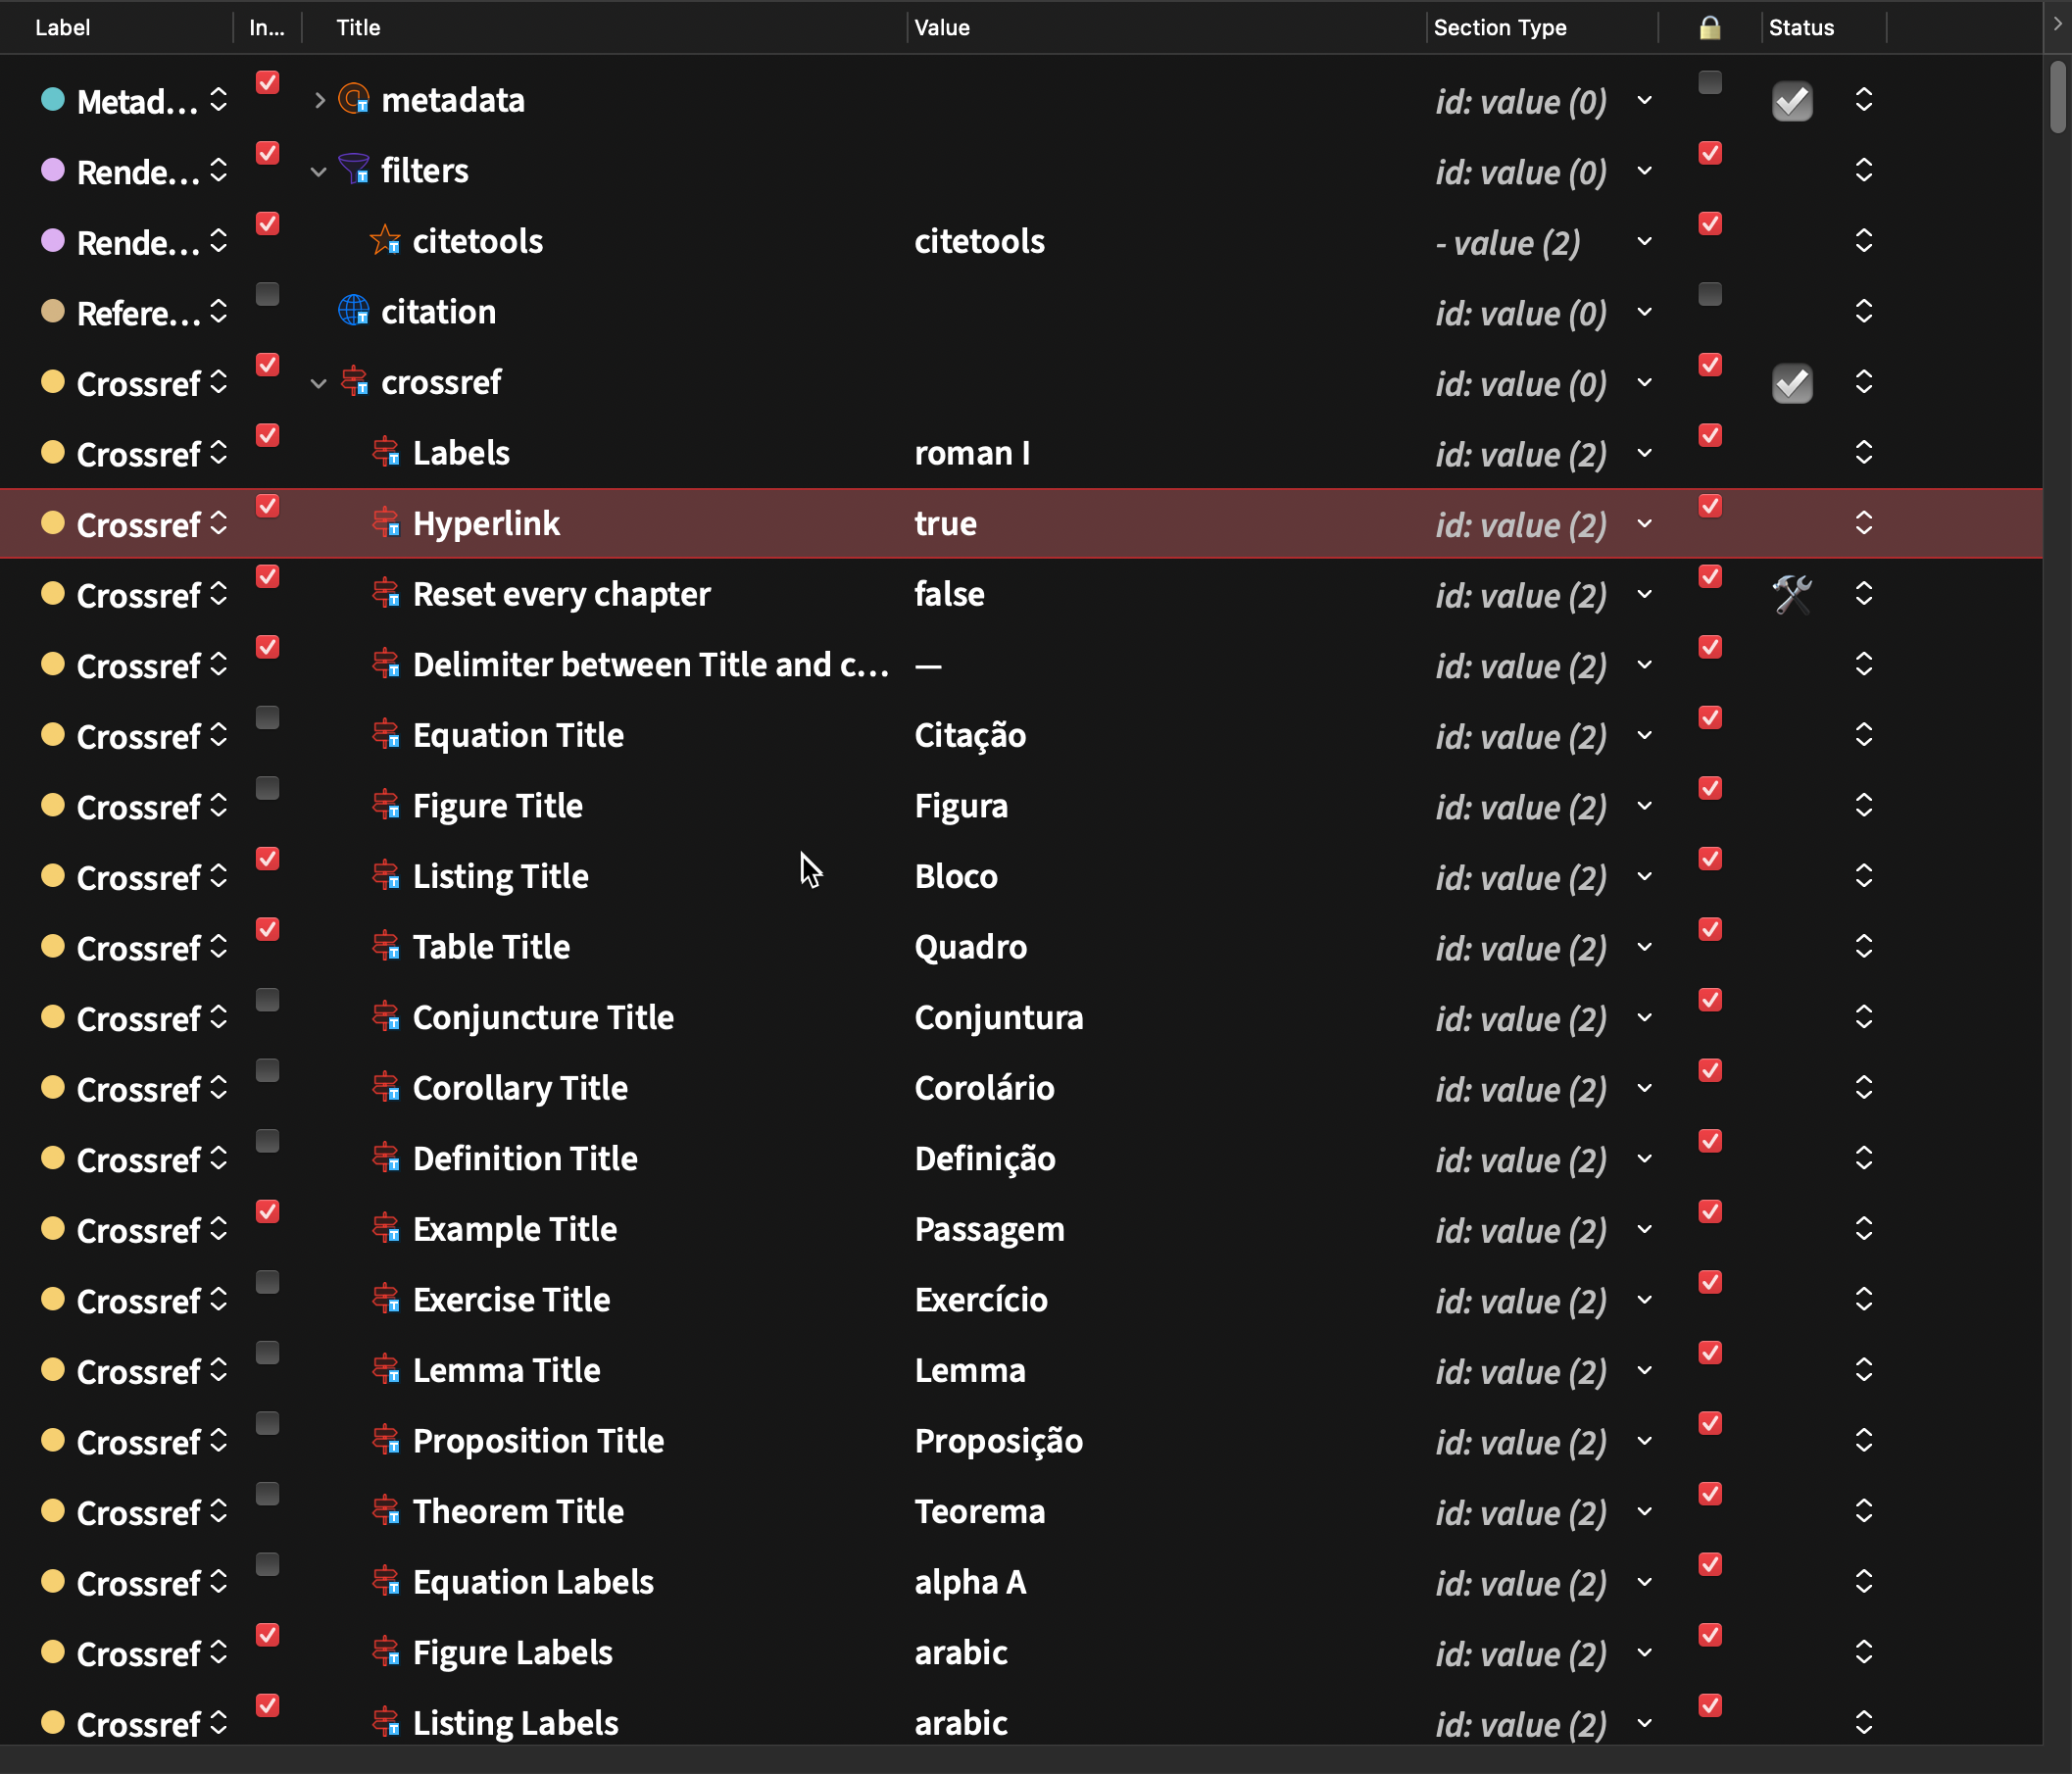
\includegraphics[width=5.20833in,height=4.36458in]{crossref.png}

}

\caption{\label{fig-scriv2A}Instead of using the \texttt{Title}, the
YAML key-value pair is usually formed by item's
\texttt{\textless{}\textbackslash{}\$custom:ID\textgreater{}}, and
\texttt{\textless{}\textbackslash{}\$custom:Value\textgreater{}} or
\texttt{Text} to allow the of more descriptive titles. The new front
matter also makes it a breeze to edit parameters without disturbing
YAML's sensitive white space rules, and it makes it much easier to
revert to a working configuration after introducing accidental errors.}

\end{figure}

\begin{figure}

{\centering 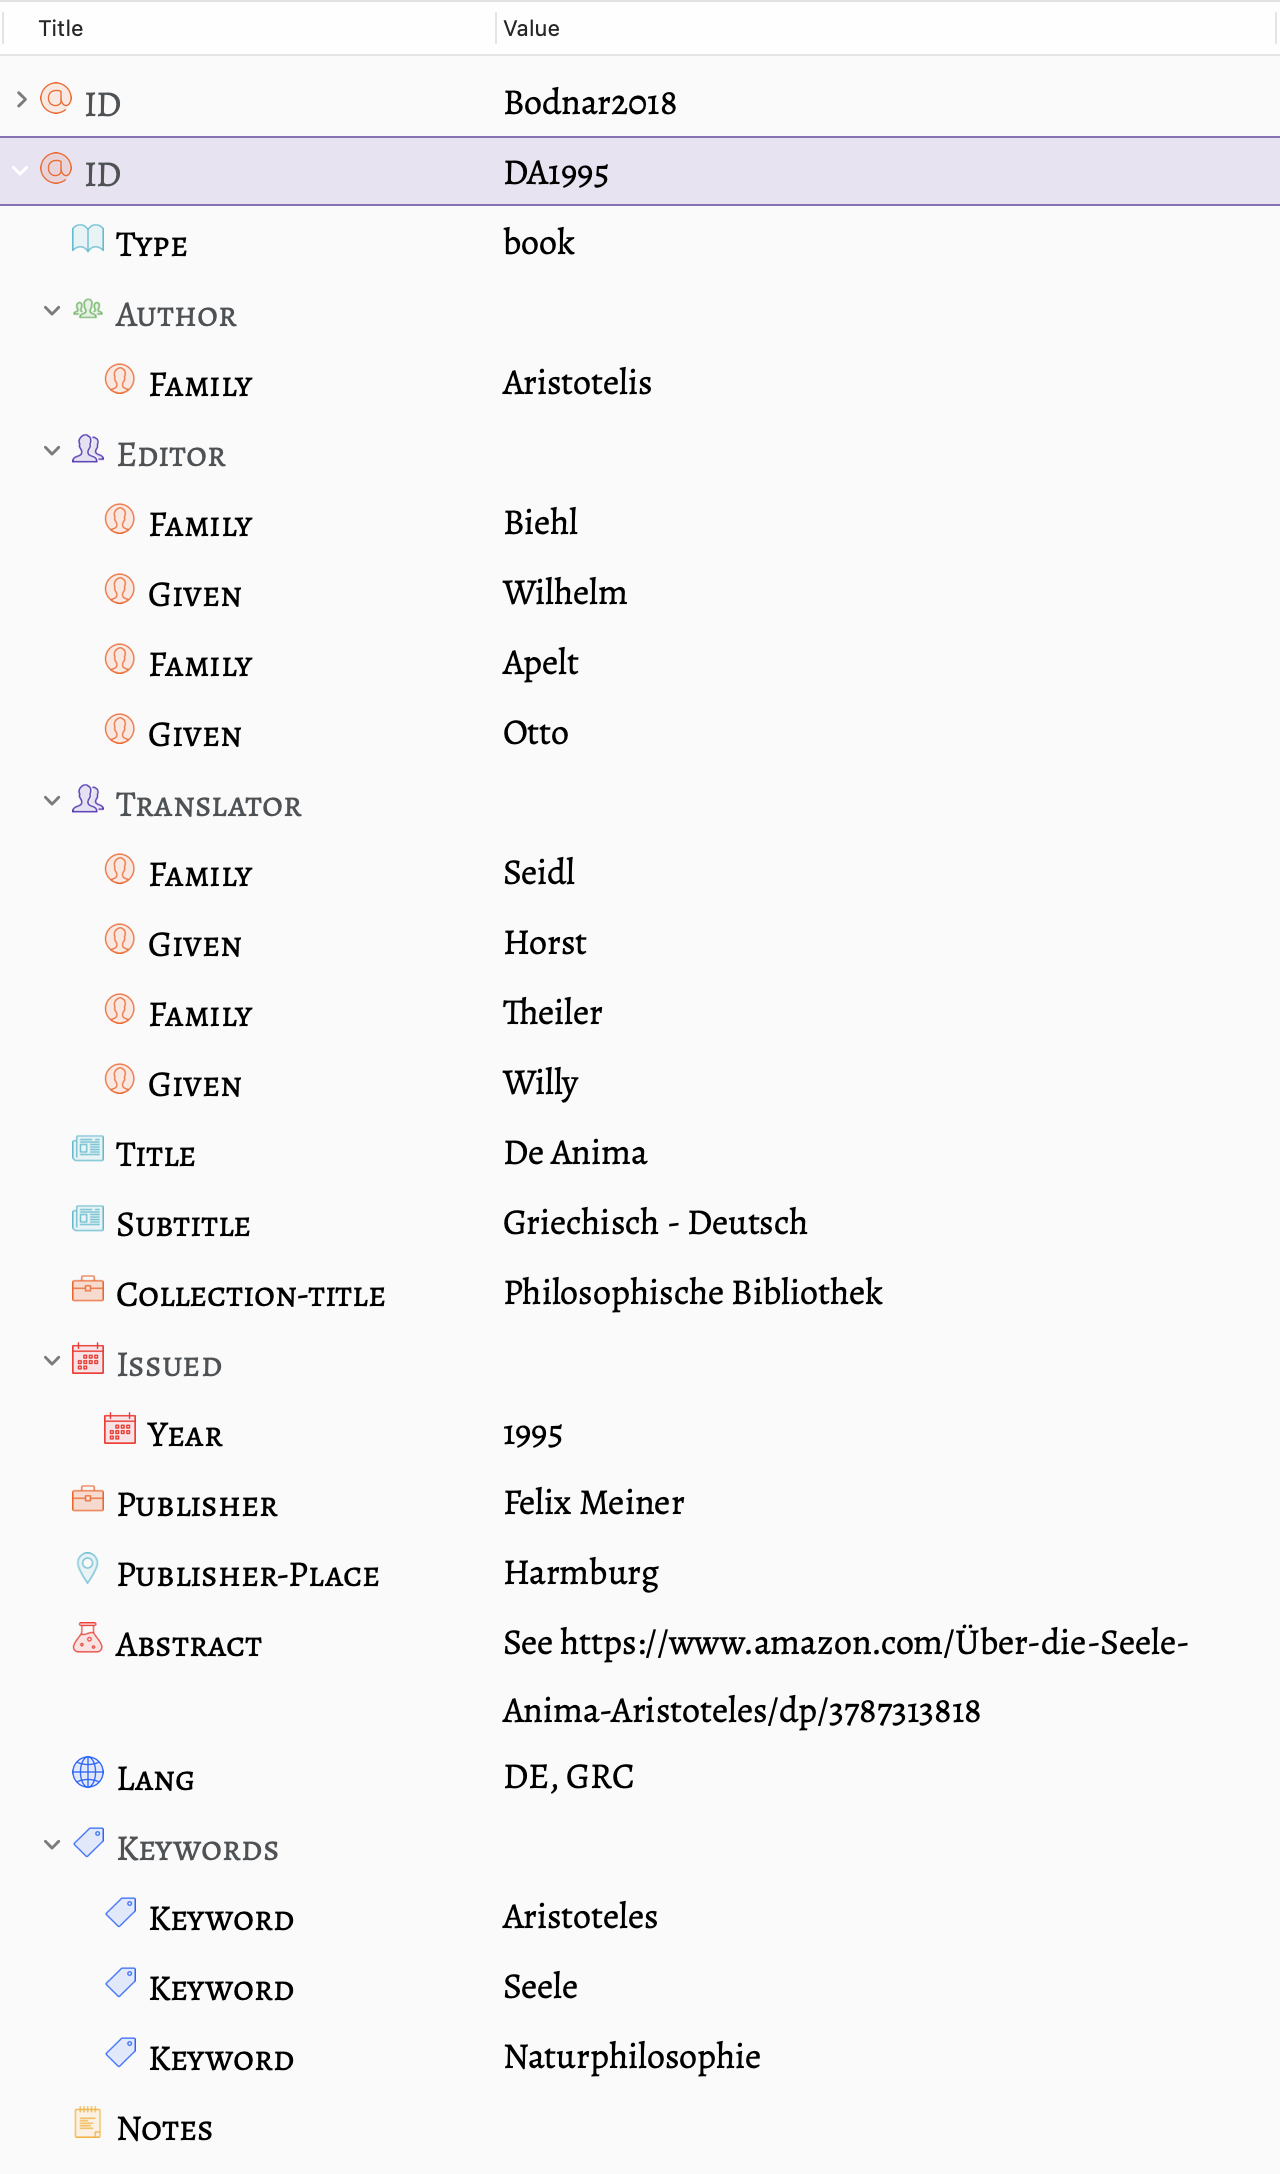
\includegraphics[width=3.66667in,height=6.25in]{cslyaml.png}

}

\caption{\label{fig-scriv2B}This demonstrates how to keep, entirely
within Scrivener, a bibliography in CSL-YAML, the format favored by
Pandoc and Quarto (being +10x faster to process than BibTeX and RIS).
You can find this sample in the templates folder.}

\end{figure}

\begin{tcolorbox}[enhanced jigsaw, left=2mm, colframe=quarto-callout-note-color-frame, bottomtitle=1mm, colback=white, coltitle=black, title=\textcolor{quarto-callout-note-color}{\faInfo}\hspace{0.5em}{A sworn of parameters}, toprule=.15mm, rightrule=.15mm, opacityback=0, breakable, toptitle=1mm, titlerule=0mm, colbacktitle=quarto-callout-note-color!10!white, arc=.35mm, bottomrule=.15mm, leftrule=.75mm, opacitybacktitle=0.6]

Many parameters are included for completeness and could be erased if
they are not in use. Should they become necessary, they can be retrieved
again from a newly created project.

\end{tcolorbox}

Looking for one way to control \textbf{Quarto} from \textbf{Scrivener},
we find not \emph{one}, but \emph{many} ways of doing so. So much that
we are reminded of Socrates addressing Meno, in the homonymous dialogue,
saying that, in looking for \emph{the} virtue of human excellence, he
had found a sworn of them coming from his interlocutor.

\begin{quote}
ΣΩ. Πολλῇ γέ τινι εὐτυχίᾳ ἔοικα κεχρῆσθαι, ὦ Μένων, εἰ μίαν ζητῶν ἀρετὴν
σμῆνός τι ἀνηύρηκα ἀρετῶν παρὰ σοὶ κειμένων
(\protect\hypertarget{cite_3}{}{\label{cite_3}(\protect\hyperlink{ref-Men}{\textbf{Men?}})}
72A-B). \enquote{\emph{I seem to be in good luck, Meno; for in seeking
one virtue I have discovered a whole swarm of virtues there in your
keeping.}}
\end{quote}

\begin{tcolorbox}[enhanced jigsaw, left=2mm, colframe=quarto-callout-caution-color-frame, bottomtitle=1mm, colback=white, coltitle=black, title=\textcolor{quarto-callout-caution-color}{\faFire}\hspace{0.5em}{Binder glitches}, toprule=.15mm, rightrule=.15mm, opacityback=0, breakable, toptitle=1mm, titlerule=0mm, colbacktitle=quarto-callout-caution-color!10!white, arc=.35mm, bottomrule=.15mm, leftrule=.75mm, opacitybacktitle=0.6]

In some cases, the sheer number of items can cause the \textbf{Binder}
to behave in strange ways. If you notice any glitches, collapse and
expand the parent item for the children to be properly displayed.
Removing unused parameters should alleviate the problem.

\end{tcolorbox}

Apart from one-click compilation, and facilitated parameter settings,
two priorities in \textbf{ScrivQ} are cross-referencing
(\protect\hypertarget{cite_4}{}{\label{cite_4}Section~\ref{sec-scriv3}})
and bibliography
(\protect\hypertarget{cite_5}{}{\label{cite_5}Section~\ref{sec-scriv42}}).

\hypertarget{sec-scriv3}{%
\chapter{Cross-referencing}\label{sec-scriv3}}

\protect\hypertarget{scriv3}{}{}

With all the affordances of \textbf{Scrivener} and \textbf{Quarto},
cross-referencing is not a trivial matter, \ul{as the options are many}.

{\marginnote{\begin{footnotesize}Automatic IDs\end{footnotesize}}}First,
bear in mind that \textbf{Section Types} and \textbf{Paragraph Styles}
(preceded by the relevant prefix, such as \emph{sec}, \emph{cnj},
\emph{cor}, \emph{def}, \emph{exm}, \emph{exr}, \emph{lem}, \emph{prp},
\emph{thm}, \emph{eq}, \emph{lst}, \emph{fig}, \emph{tbl}) are rigged
with automatic IDs in the format
\texttt{scriv\textless{}\textbackslash{}\$linkID\textgreater{}}\footnote{Note
  that in Scrivener we have to escape the \texttt{\$}, otherwise the
  placeholder will get expanded into its correct value during
  compilation.}. This way, there is no need to choose an ID each time an
element is created, nor to remember any when another needs to be
referenced (to create links we will use this same standard identifier,
\texttt{scriv\textless{}\textbackslash{}\$linkID\textgreater{}}, select
the text, link to the appropriate document, and apply the style
corresponding to the element we want to reference). We leave it to
Scrivener to figure out the value of the
\texttt{\textless{}\textbackslash{}\$linkID\textgreater{}} placeholder.

\begin{tcolorbox}[enhanced jigsaw, left=2mm, colframe=quarto-callout-note-color-frame, bottomtitle=1mm, colback=white, coltitle=black, title=\textcolor{quarto-callout-note-color}{\faInfo}\hspace{0.5em}{Translating Quarto into Scrivener}, toprule=.15mm, rightrule=.15mm, opacityback=0, breakable, toptitle=1mm, titlerule=0mm, colbacktitle=quarto-callout-note-color!10!white, arc=.35mm, bottomrule=.15mm, leftrule=.75mm, opacitybacktitle=0.6]

In \textbf{ScrivQ} we can use \textbf{Section Types} or
\textbf{Paragraph Styles} to create \textbf{Sections}, \textbf{Tables},
\textbf{Equations}, \textbf{Figures}, \textbf{Listings},
\textbf{Callouts} (Caution, Important, Note, Tip, Warning), and
\textbf{Amsthm} environments (Conjecture, Corollary, Definition,
Example, Exercise, Lemma, Proposition, Theorem). We can also use
\textbf{Character Styles} to easily reference any of them. Keep reading
to learn how.

\end{tcolorbox}

\begin{tcolorbox}[enhanced jigsaw, left=2mm, colframe=quarto-callout-tip-color-frame, bottomtitle=1mm, colback=white, coltitle=black, title=\textcolor{quarto-callout-tip-color}{\faLightbulb}\hspace{0.5em}{Choosing your own label for automatic links}, toprule=.15mm, rightrule=.15mm, opacityback=0, breakable, toptitle=1mm, titlerule=0mm, colbacktitle=quarto-callout-tip-color!10!white, arc=.35mm, bottomrule=.15mm, leftrule=.75mm, opacitybacktitle=0.6]

In \textbf{ScrivQ} one can use different keywords as labels for
automatic links. Simply use one of the provided rules for
\textbf{Replacements}
(\protect\hypertarget{cite_6}{}{\label{cite_6}Figure~\ref{fig-scriv3}})
in the Compile settings (or in the Format configurations) to have
keywords such as \texttt{scriv} + \texttt{link}, \texttt{autο} +
\texttt{ref}, \texttt{\%autο} + \texttt{ref\%}, \texttt{\%autοref:} +
\texttt{something-random-that-will-be-erased\%}, \texttt{{[}autοref{]}},
converted into
\texttt{scriv\textless{}\textbackslash{}\$linkID\textgreater{}} during
compilation.

\end{tcolorbox}

\begin{figure}

{\centering 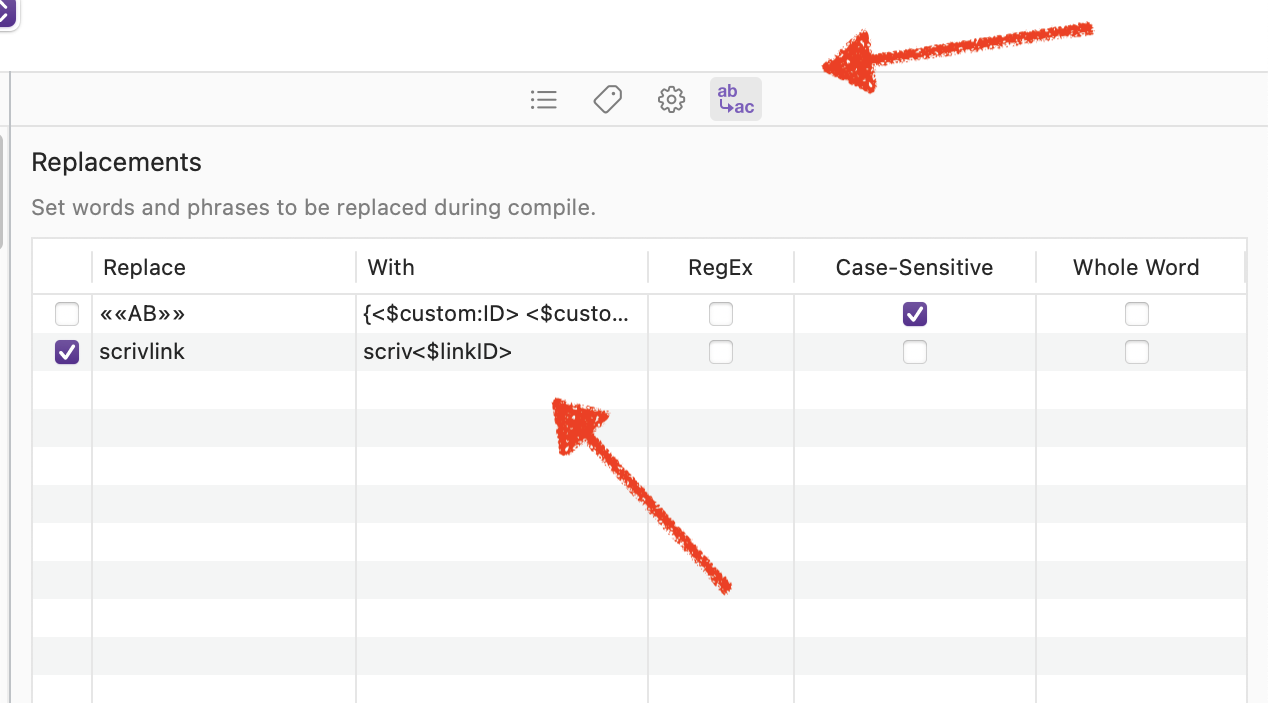
\includegraphics[width=4.30208in,height=2.38542in]{Replacements.png}

}

\caption{\label{fig-scriv3}\textbf{Replacements} pane in the
\textbf{Compile\ldots{}} configurations can be used to allow different
labels for automatic links. This is purely optional and we recommend
limiting this to one rule or two.}

\end{figure}

{\marginnote{\begin{footnotesize}Add prefix and markup using Character
Styles\end{footnotesize}}}To cross-reference a \texttt{table}, an
\texttt{example}, or a \texttt{theorem}, one could use
\texttt{tbl-keyword} (\emph{i.e.}
\texttt{tbl-scriv\textless{}\textbackslash{}\$linkID\textgreater{}}),
\texttt{exm-keyword} (\emph{i.e.}
\texttt{exm-scriv\textless{}\textbackslash{}\$linkID\textgreater{}}),
and \texttt{thm-keyword} (\emph{i.e.}
\texttt{thm-scriv\textless{}\textbackslash{}\$linkID\textgreater{}}),
respectively. Seeing that the prefixes are not always easy to remember,
\textbf{Character Styles} are available to inject the correct markup.

The \texttt{Crossref} \texttt{Table}, for example, will turn the
\texttt{keyword} into \texttt{{[}@tbl-keyword{]}}\footnote{That is,
  \texttt{{[}@tbl-scriv\textless{}\textbackslash{}\$linkID\textgreater{}{]}}.}\texttt{;}
and the \texttt{Crossref\ Table\textbackslash{}*} style will turn it
into \texttt{{[}@tbl-keyword{]}}\footnote{That is,
  \texttt{{[}-@tbl-scriv\textless{}\textbackslash{}\$linkID\textgreater{}{]}}.}.
{\marginnote{\begin{footnotesize}The asterisk (\texttt{*}) in the title
of Character Styles indicates the suppression of part of the data (as is
common in LaTeX).\end{footnotesize}}} Likewise, the
\texttt{Crossref\ Example} and the
\texttt{Crossref\ Example\textbackslash{}*} which will result in
\texttt{{[}@exm-keyword{]}} and \texttt{{[}-@exm-keyword{]}}\footnote{That
  is,
  \texttt{{[}@exm-scriv\textless{}\textbackslash{}\$linkID\textgreater{}{]}}
  and
  \texttt{{[}-@exm-scriv\textless{}\textbackslash{}\$linkID\textgreater{}{]}}.},
and so on. See \emph{scriv4} below for yet more examples.

\begin{tcolorbox}[enhanced jigsaw, left=2mm, colframe=quarto-callout-tip-color-frame, bottomtitle=1mm, colback=white, coltitle=black, title=\textcolor{quarto-callout-tip-color}{\faLightbulb}\hspace{0.5em}{Cross-referencing a table}, toprule=.15mm, rightrule=.15mm, opacityback=0, breakable, toptitle=1mm, titlerule=0mm, colbacktitle=quarto-callout-tip-color!10!white, arc=.35mm, bottomrule=.15mm, leftrule=.75mm, opacitybacktitle=0.6]

\begin{enumerate}
\def\labelenumi{\arabic{enumi}.}
\tightlist
\item
  \texttt{Type} \texttt{your-keyword-of-choice} or
  \texttt{scriv\textless{}\textbackslash{}\$linkID\textgreater{}},
  \texttt{select} it, and hit \texttt{Command\ +\ L};
\item
  \texttt{Link} to the document that contains the table.
  (\emph{e.g}\textbf{.} scriv13);
\item
  Apply a \textbf{Character Style} called \texttt{Crossref\ Table}
  (\emph{e.g.}
  \protect\hypertarget{cite_7}{}{\label{cite_7}Table~\ref{tbl-scriv13}}).
\end{enumerate}

\end{tcolorbox}

Below we will see several examples of the same strategy being applied to
several different elements. I hope that these examples prove as
instructive to consult as they were to prepare.

\hypertarget{sec-scriv4}{%
\section{Amsthm}\label{sec-scriv4}}

\protect\hypertarget{scriv4}{}{}

In this section, we are demonstrating the cross-referencing mechanism
working with \textbf{Amsthm} theorems. First, we will see all of the
theorems created using \textbf{Paragraph Styles}, then they will be
introduced again as \textbf{Section Types}. In the table below, you'll
see several Character Styles (labeled as \texttt{Crossref...}) used to
reference both.

\begin{longtable}[]{@{}ccc@{}}
\toprule\noalign{}
\textbf{Element} & \textbf{Markdown Source} & \textbf{Rendered
Output} \\
\midrule\noalign{}
\endhead
\bottomrule\noalign{}
\endlastfoot
Conjecture & \texttt{{[}@cnj-scriv4{]}} &
\protect\hypertarget{cite_8}{}{\label{cite_8}Conjecture~\ref{cnj-scriv4}} \\
Conjecture & \texttt{{[}@cnj-scriv5{]}} &
\protect\hypertarget{cite_9}{}{\label{cite_9}Conjecture~\ref{cnj-scriv5}} \\
Corollary & \texttt{{[}@cor-scriv4{]}} &
\protect\hypertarget{cite_10}{}{\label{cite_10}Corollary~\ref{cor-scriv4}} \\
Corollary & \texttt{{[}@cor-scriv6{]}} &
\protect\hypertarget{cite_11}{}{\label{cite_11}Corollary~\ref{cor-scriv6}} \\
Definition & \texttt{{[}@def-scriv4{]}} &
\protect\hypertarget{cite_12}{}{\label{cite_12}Definition~\ref{def-scriv4}} \\
Definition & \texttt{{[}@def-scriv7{]}} &
\protect\hypertarget{cite_13}{}{\label{cite_13}Definition~\ref{def-scriv7}} \\
Example & \texttt{{[}@exm-scriv4{]}} &
\protect\hypertarget{cite_14}{}{\label{cite_14}Example~\ref{exm-scriv4}} \\
Example & \texttt{{[}@exm-scriv8{]}} &
\protect\hypertarget{cite_15}{}{\label{cite_15}Example~\ref{exm-scriv8}} \\
Exercise & \texttt{{[}@exr-scriv4{]}} &
\protect\hypertarget{cite_16}{}{\label{cite_16}Exercise~\ref{exr-scriv4}} \\
Exercise & \texttt{{[}@exr-scriv9{]}} &
\protect\hypertarget{cite_17}{}{\label{cite_17}Exercise~\ref{exr-scriv9}} \\
Lemma & \texttt{{[}@lem-scriv4{]}} &
\protect\hypertarget{cite_18}{}{\label{cite_18}Lemma~\ref{lem-scriv4}} \\
Lemma & \texttt{{[}@lem-scriv10{]}} &
\protect\hypertarget{cite_19}{}{\label{cite_19}Lemma~\ref{lem-scriv10}} \\
Proposition & \texttt{{[}@prp-scriv4{]}} &
\protect\hypertarget{cite_20}{}{\label{cite_20}Proposition~\ref{prp-scriv4}} \\
Proposition & \texttt{{[}@prp-scriv11{]}} &
\protect\hypertarget{cite_21}{}{\label{cite_21}Proposition~\ref{prp-scriv11}} \\
Theorem & \texttt{{[}@thm-scriv4{]}} &
\protect\hypertarget{cite_22}{}{\label{cite_22}Theorem~\ref{thm-scriv4}} \\
Theorem & \texttt{{[}@thm-scriv12{]}} &
\protect\hypertarget{cite_23}{}{\label{cite_23}Theorem~\ref{thm-scriv12}} \\
\end{longtable}

\textbf{Paragraph Styles}

\begin{conjecture}[]\protect\hypertarget{cnj-scriv4}{}\label{cnj-scriv4}

Conjecture

\end{conjecture}

\begin{corollary}[]\protect\hypertarget{cor-scriv4}{}\label{cor-scriv4}

Corollary

\end{corollary}

\begin{definition}[]\protect\hypertarget{def-scriv4}{}\label{def-scriv4}

Definition

\end{definition}

\begin{example}[]\protect\hypertarget{exm-scriv4}{}\label{exm-scriv4}

Example

\end{example}

\begin{exercise}[]\protect\hypertarget{exr-scriv4}{}\label{exr-scriv4}

Exercise

\end{exercise}

\begin{lemma}[]\protect\hypertarget{lem-scriv4}{}\label{lem-scriv4}

Lemma

\end{lemma}

\begin{proposition}[]\protect\hypertarget{prp-scriv4}{}\label{prp-scriv4}

Proposition

\end{proposition}

\begin{theorem}[]\protect\hypertarget{thm-scriv4}{}\label{thm-scriv4}

Let (f) be a function whose derivative exists in every point, then (f)
is a continuous function. \textbackslash end\{theorem\}

\begin{theorem}[Pythagorean theorem]
\label{pythagorean}
This is a theorem about right triangles and can be summarised in the next 
equation 
\[ x^2 + y^2 = z^2 \]
\end{theorem}

And a consequence of theorem \ref{pythagorean} is the statement in the
next corollary.

\begin{corollary}
There's no right rectangle whose sides measure 3cm, 4cm, and 6cm.
\end{corollary}

You can reference theorems such as \ref{pythagorean} when a label is
assigned.

\begin{lemma}
Given two line segments whose lengths are \(a\) and \(b\) respectively there is a 
real number \(r\) such that \(b=ra\).
\end{lemma}

\end{theorem}

\begin{conjecture}[]\protect\hypertarget{cnj-scriv4}{}\label{cnj-scriv4}

Conjecture

\end{conjecture}

\begin{corollary}[]\protect\hypertarget{cor-scriv4}{}\label{cor-scriv4}

Corollary

\end{corollary}

\begin{definition}[]\protect\hypertarget{def-scriv4}{}\label{def-scriv4}

Definition

\end{definition}

\begin{example}[]\protect\hypertarget{exm-scriv4}{}\label{exm-scriv4}

Example

\end{example}

\begin{exercise}[]\protect\hypertarget{exr-scriv4}{}\label{exr-scriv4}

Exercise

\end{exercise}

\begin{lemma}[]\protect\hypertarget{lem-scriv4}{}\label{lem-scriv4}

Lemma

\end{lemma}

\begin{proposition}[]\protect\hypertarget{prp-scriv4}{}\label{prp-scriv4}

Proposition

\end{proposition}

\begin{theorem}[]\protect\hypertarget{thm-scriv4}{}\label{thm-scriv4}

Theorem

\end{theorem}

\textbf{Section Types}

\begin{conjecture}[]\protect\hypertarget{cnj-scriv5}{}\label{cnj-scriv5}

Conjecture

\end{conjecture}

\begin{corollary}[]\protect\hypertarget{cor-scriv6}{}\label{cor-scriv6}

Corollary

\end{corollary}

\begin{definition}[]\protect\hypertarget{def-scriv7}{}\label{def-scriv7}

Definition

\end{definition}

\begin{example}[]\protect\hypertarget{exm-scriv8}{}\label{exm-scriv8}

Example

\end{example}

\begin{exercise}[]\protect\hypertarget{exr-scriv9}{}\label{exr-scriv9}

Exercise

\end{exercise}

\begin{lemma}[]\protect\hypertarget{lem-scriv10}{}\label{lem-scriv10}

Lemma

\end{lemma}

\begin{proposition}[]\protect\hypertarget{prp-scriv11}{}\label{prp-scriv11}

Proposition

\end{proposition}

\begin{theorem}[]\protect\hypertarget{thm-scriv12}{}\label{thm-scriv12}

Theorem

\end{theorem}

\hypertarget{sec-scriv13}{%
\section{Block Elements}\label{sec-scriv13}}

\protect\hypertarget{scriv13}{}{}

Now we repeat the same approach we saw with the \textbf{Amsthm} theorems
with other \textbf{Quarto} and \textbf{Pandoc} block elements, such as
computations (diagrams), equations, listings, figures, and tables. This
time, apart from \textbf{Paragraph Styles} and \textbf{Section Types},
we will also use \texttt{Raw\ Markdown} to accomplish the same tasks. As
before, all of these elements receive automatic IDs.

\hypertarget{tbl-scriv13}{}
\begin{longtable}[]{@{}ccc@{}}
\toprule\noalign{}
\textbf{Element} & \textbf{Markdown Source} & \textbf{Rendered
Output} \\
\midrule\noalign{}
\endfirsthead
\toprule\noalign{}
\textbf{Element} & \textbf{Markdown Source} & \textbf{Rendered
Output} \\
\midrule\noalign{}
\endhead
\bottomrule\noalign{}
\endlastfoot
Diagram & \texttt{{[}@fig-scriv16{]}} &
\protect\hypertarget{cite_24}{}{\label{cite_24}Figure~\ref{fig-scriv16}} \\
Diagram & \texttt{{[}@fig-scriv16B{]}} &
\protect\hypertarget{cite_25}{}{\label{cite_25}Figure~\ref{fig-scriv16B}} \\
Diagram & \texttt{{[}@fig-scriv17{]}} &
\protect\hypertarget{cite_26}{}{\label{cite_26}Figure~\ref{fig-scriv17}} \\
Diagram & \texttt{{[}@fig-scriv18{]}} &
\protect\hypertarget{cite_27}{}{\label{cite_27}Figure~\ref{fig-scriv18}} \\
Diagram & \texttt{{[}@fig-scriv18B{]}} &
\protect\hypertarget{cite_28}{}{\label{cite_28}Figure~\ref{fig-scriv18B}} \\
Diagram & \texttt{{[}@fig-scriv19{]}} &
\protect\hypertarget{cite_29}{}{\label{cite_29}Figure~\ref{fig-scriv19}} \\
Equation & \texttt{{[}@eq-scriv21{]}} &
\protect\hypertarget{cite_30}{}{\label{cite_30}Equation~\ref{eq-scriv21}} \\
Equation & \texttt{{[}@eq-scriv22{]}} &
\protect\hypertarget{cite_31}{}{\label{cite_31}Equation~\ref{eq-scriv22}} \\
Figure & \texttt{{[}@fig-scriv24{]}} &
\protect\hypertarget{cite_32}{}{\label{cite_32}Figure~\ref{fig-scriv24}} \\
Figure (Multipart) & \texttt{{[}@fig-scriv25{]}} &
\protect\hypertarget{cite_33}{}{\label{cite_33}Figure~\ref{fig-scriv25}} \\
Figure (Multipart) & \texttt{{[}@fig-scriv25A{]}} &
\protect\hypertarget{cite_34}{}{\label{cite_34}Figure~\ref{fig-scriv25A}} \\
Figure (Multipart) & \texttt{{[}@fig-scriv25B{]}} &
\protect\hypertarget{cite_35}{}{\label{cite_35}Figure~\ref{fig-scriv25B}} \\
Figure (Multipart) & \texttt{{[}@fig-scriv26{]}} &
\protect\hypertarget{cite_36}{}{\label{cite_36}Figure~\ref{fig-scriv26}} \\
Figure (Multipart) & \texttt{{[}@fig-scriv26A{]}} &
\protect\hypertarget{cite_37}{}{\label{cite_37}Figure~\ref{fig-scriv26A}} \\
Figure (Multipart) & \texttt{{[}@fig-scriv26B{]}} &
\protect\hypertarget{cite_38}{}{\label{cite_38}Figure~\ref{fig-scriv26B}} \\
Listing & \texttt{{[}@lst-scriv28{]}} &
\protect\hypertarget{cite_39}{}{\label{cite_39}Listing~\ref{lst-scriv28}} \\
Listing & \texttt{{[}@lst-scriv29{]}} &
\protect\hypertarget{cite_40}{}{\label{cite_40}Listing~\ref{lst-scriv29}} \\
Table & \texttt{{[}@tbl-scriv31{]}} &
\protect\hypertarget{cite_41}{}{\label{cite_41}Table~\ref{tbl-scriv31}} \\
Table & \texttt{{[}@tbl-scriv32{]}} &
\protect\hypertarget{cite_42}{}{\label{cite_42}Table~\ref{tbl-scriv32}} \\
Table (Multipart) & \texttt{{[}@tbl-scriv33{]}} &
\protect\hypertarget{cite_43}{}{\label{cite_43}Table~\ref{tbl-scriv33}} \\
Table (Multipart) & \texttt{{[}@tbl-scriv33A{]}} &
\protect\hypertarget{cite_44}{}{\label{cite_44}Table~\ref{tbl-scriv33A}} \\
Table (Multipart) & \texttt{{[}@tbl-scriv33B{]}} &
\protect\hypertarget{cite_45}{}{\label{cite_45}Table~\ref{tbl-scriv33B}} \\
\caption{\label{tbl-scriv13}Cross-referencing diagrams, figures,
listings and tables.}\tabularnewline
\end{longtable}

\hypertarget{sec-scriv14}{%
\subsection{Computations}\label{sec-scriv14}}

\protect\hypertarget{scriv14}{}{}

To use computations, there might be additional steps involved, such as
installing R along with additional packages.

install.packages(\enquote{reticulate})
install.packages(\enquote{markdown})
install.packages(\enquote{tidyverse})
install.packages(\enquote{kableExtra}) downlit, xml2

\hypertarget{tbl-scriv14}{}
\begin{longtable}[]{@{}ccc@{}}
\toprule\noalign{}
\textbf{Element} & \textbf{Markdown Source} & \textbf{Rendered
Output} \\
\midrule\noalign{}
\endfirsthead
\toprule\noalign{}
\textbf{Element} & \textbf{Markdown Source} & \textbf{Rendered
Output} \\
\midrule\noalign{}
\endhead
\bottomrule\noalign{}
\endlastfoot
R Computation & \texttt{{[}@fig-scriv?{]}} &
\protect\hypertarget{cite_46}{}{\label{cite_46}\textbf{?@fig-scriv}} \\
R Computation & \texttt{{[}@fig-scriv?{]}} &
\protect\hypertarget{cite_47}{}{\label{cite_47}\textbf{?@fig-scriv}} \\
Python Computation & \texttt{{[}@fig-scriv?{]}} &
\protect\hypertarget{cite_48}{}{\label{cite_48}\textbf{?@fig-scriv}} \\
Python Computation & \texttt{{[}@fig-scriv?{]}} &
\protect\hypertarget{cite_49}{}{\label{cite_49}\textbf{?@fig-scriv}} \\
\caption{\label{tbl-scriv14}Cross-referencing \textbf{R Computations}
and \textbf{Python Computations}.}\tabularnewline
\end{longtable}

\hypertarget{sec-scriv15}{%
\subsection{Diagrams}\label{sec-scriv15}}

\protect\hypertarget{scriv15}{}{}

Let us see how we can use \textbf{raw markup}, \textbf{Section Types},
and \textbf{Paragraph Styles} to create \textbf{Dot} and
\textbf{Mermaid} diagrams.

\hypertarget{tbl-scriv15}{}
\begin{longtable}[]{@{}ccc@{}}
\toprule\noalign{}
\textbf{Element} & \textbf{Markdown Source} & \textbf{Rendered
Output} \\
\midrule\noalign{}
\endfirsthead
\toprule\noalign{}
\textbf{Element} & \textbf{Markdown Source} & \textbf{Rendered
Output} \\
\midrule\noalign{}
\endhead
\bottomrule\noalign{}
\endlastfoot
Diagram Dot & \texttt{{[}@fig-scriv16{]}} &
\protect\hypertarget{cite_50}{}{\label{cite_50}Figure~\ref{fig-scriv16}} \\
Diagram Dot & \texttt{{[}@fig-scriv16B{]}} &
\protect\hypertarget{cite_51}{}{\label{cite_51}Figure~\ref{fig-scriv16B}} \\
Diagram Dot & \texttt{{[}@fig-scriv17{]}} &
\protect\hypertarget{cite_52}{}{\label{cite_52}Figure~\ref{fig-scriv17}} \\
Diagram Mermaid & \texttt{{[}@fig-scriv18{]}} &
\protect\hypertarget{cite_53}{}{\label{cite_53}Figure~\ref{fig-scriv18}} \\
Diagram Mermaid & \texttt{{[}@fig-scriv18B{]}} &
\protect\hypertarget{cite_54}{}{\label{cite_54}Figure~\ref{fig-scriv18B}} \\
Diagram Mermaid & \texttt{{[}@fig-scriv19{]}} &
\protect\hypertarget{cite_55}{}{\label{cite_55}Figure~\ref{fig-scriv19}} \\
\caption{\label{tbl-scriv15}Cross-referencing \textbf{Dot Diagrams} and
\textbf{Mermaid Diagrams}.}\tabularnewline
\end{longtable}

\begin{figure}

{\centering 

\begin{figure}[H]

{\centering 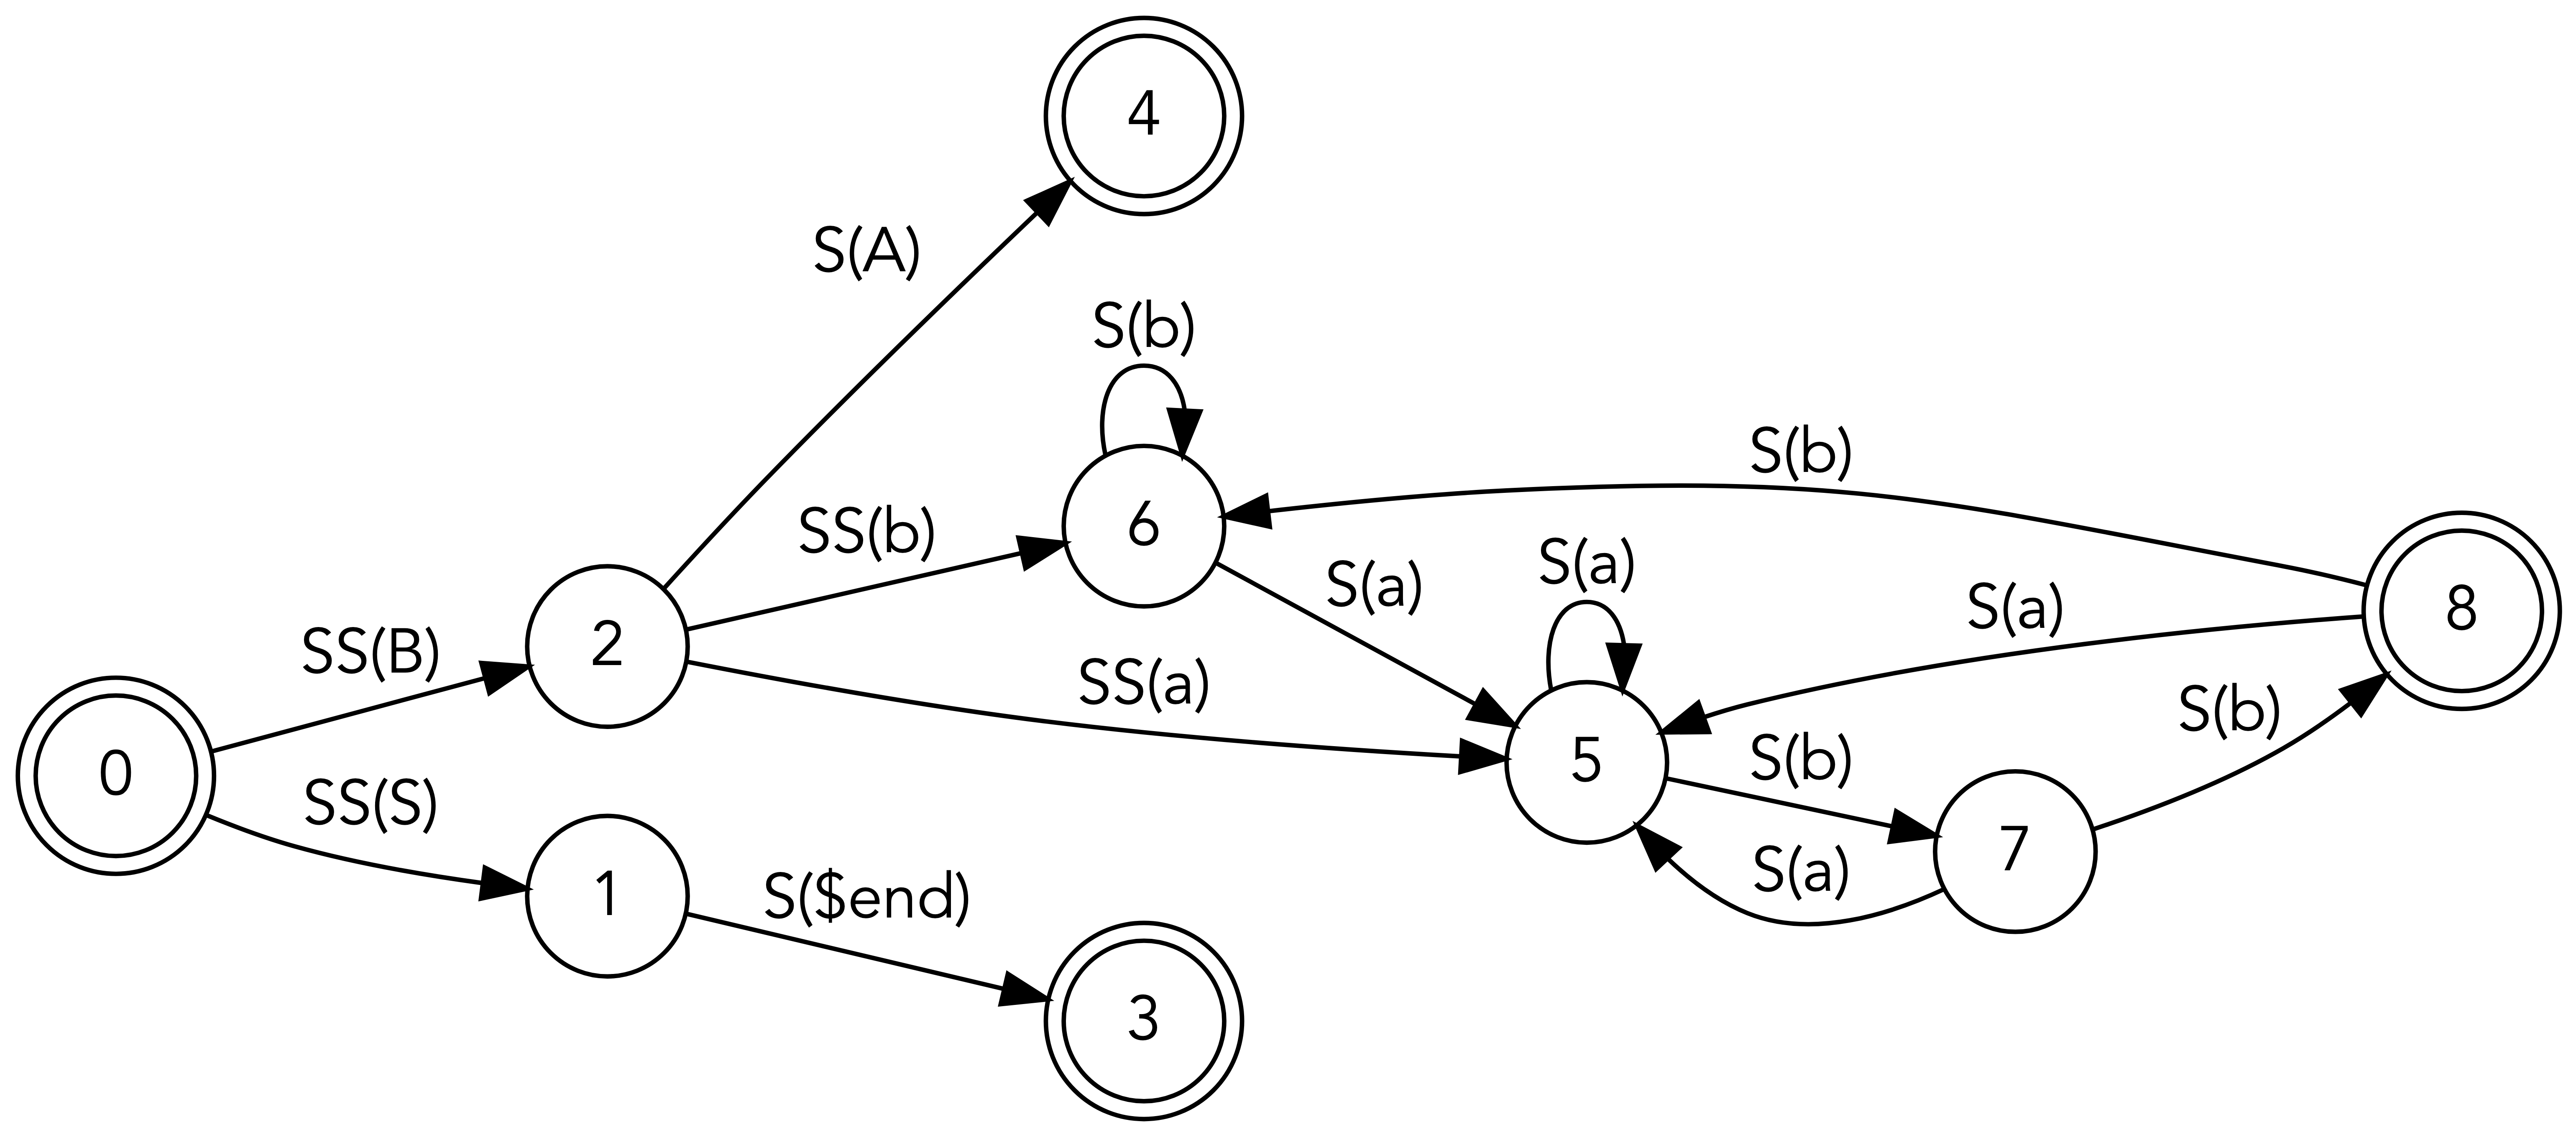
\includegraphics[width=5.5in,height=3.5in]{index_files/figure-latex/dot-figure-1.png}

}

\end{figure}

}

\caption{\label{fig-scriv16}Figure caption}

\end{figure}

\begin{figure}

{\centering 

\begin{figure}[H]

{\centering 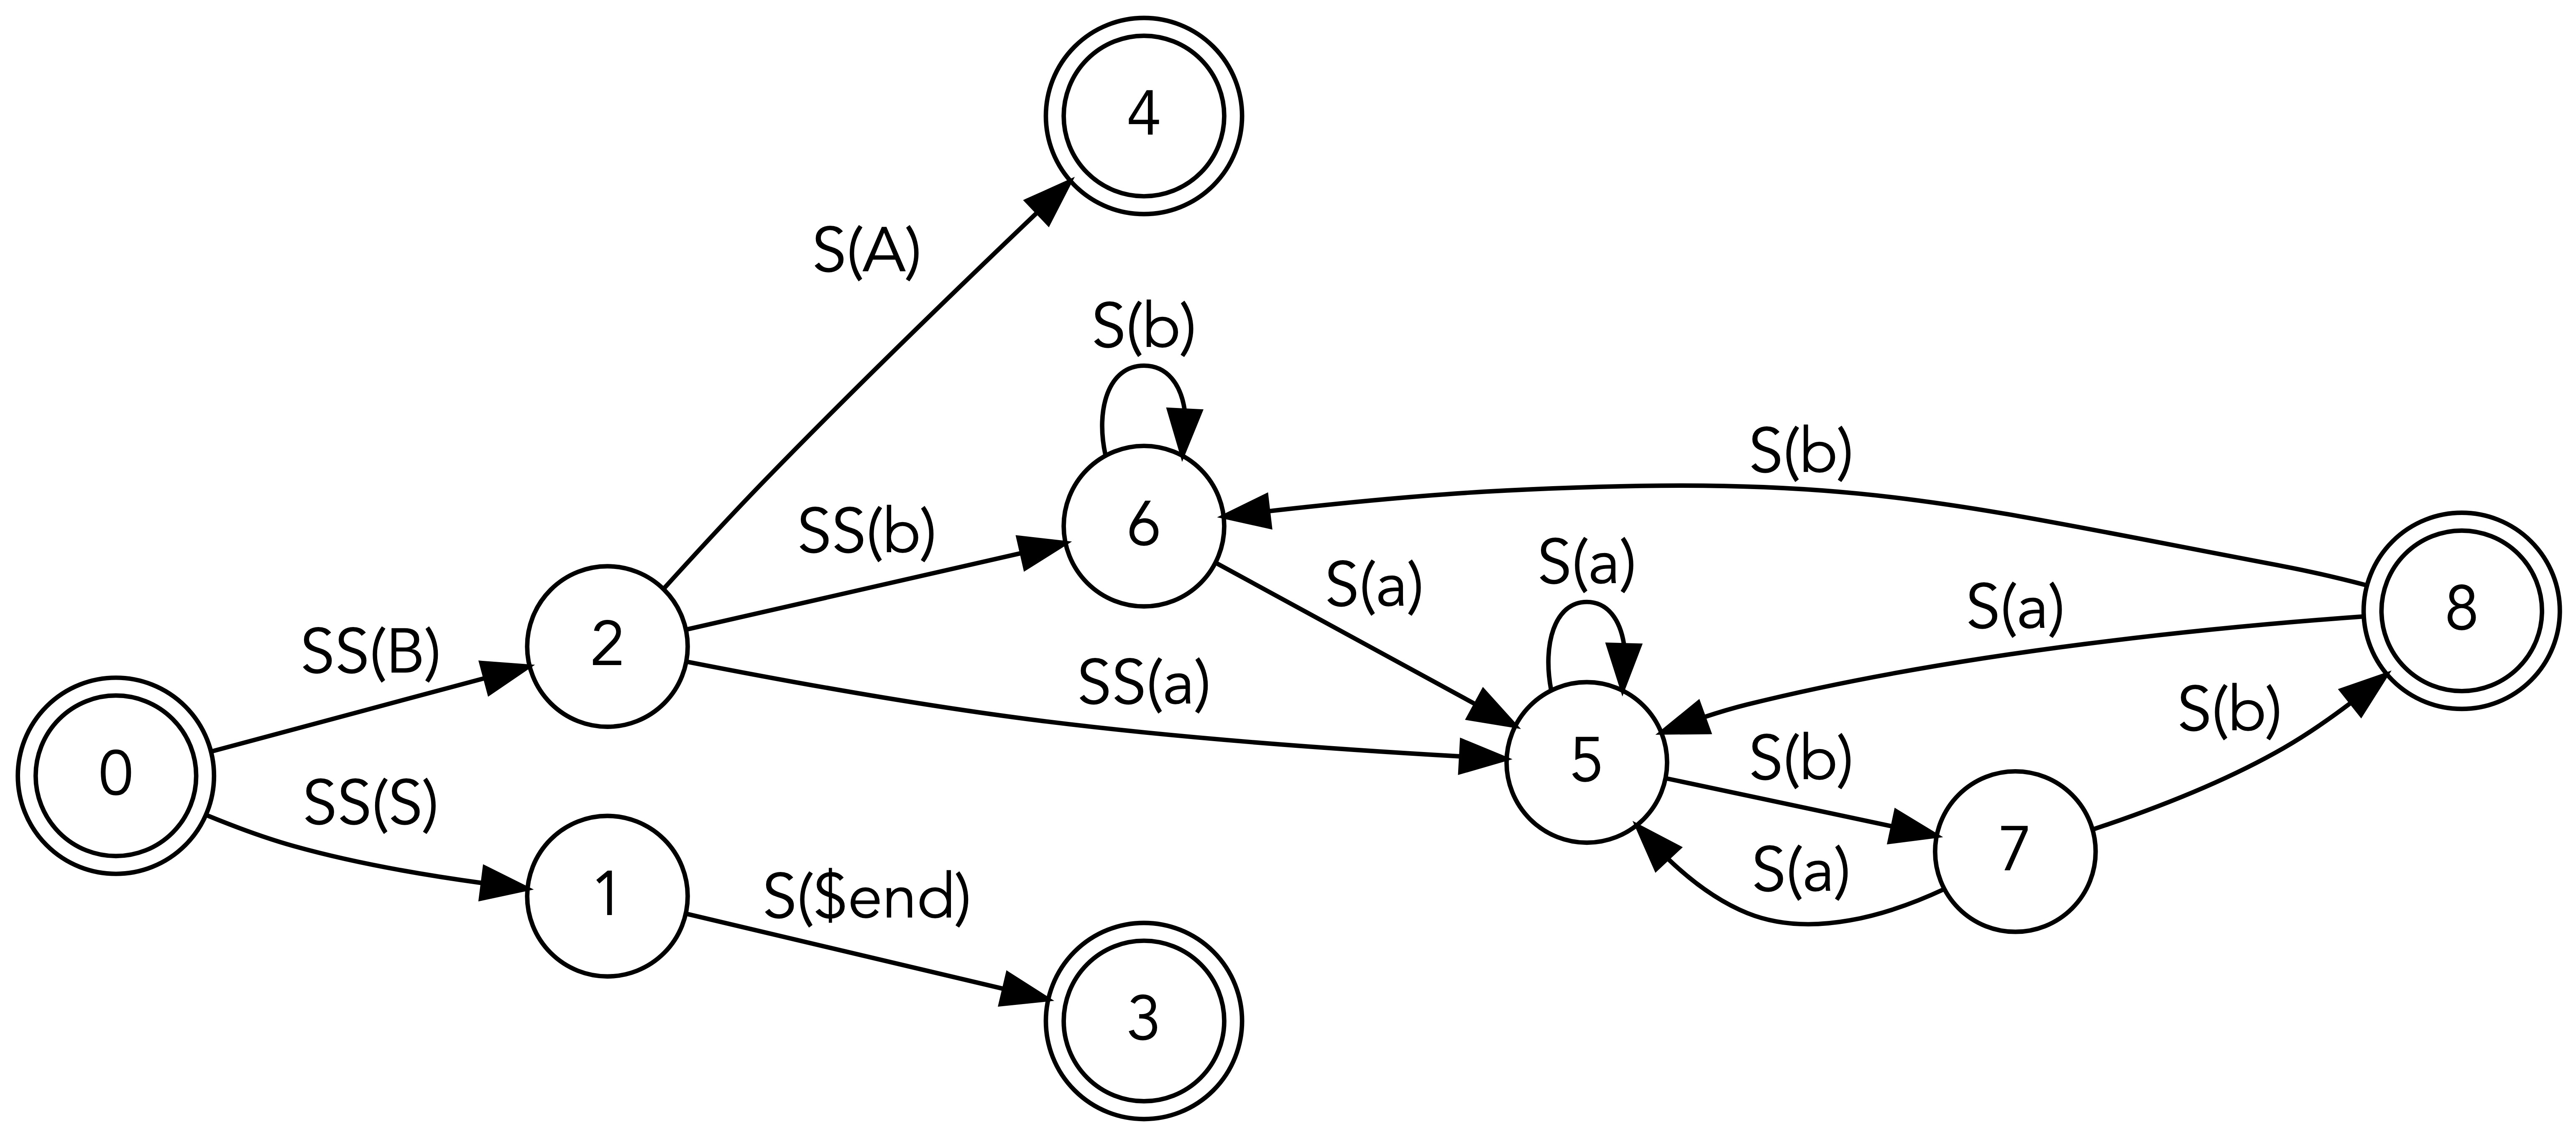
\includegraphics[width=5.5in,height=3.5in]{index_files/figure-latex/dot-figure-5.png}

}

\end{figure}

}

\caption{\label{fig-scriv16B}Figure caption}

\end{figure}

\begin{figure}

{\centering 

\begin{figure}[H]

{\centering 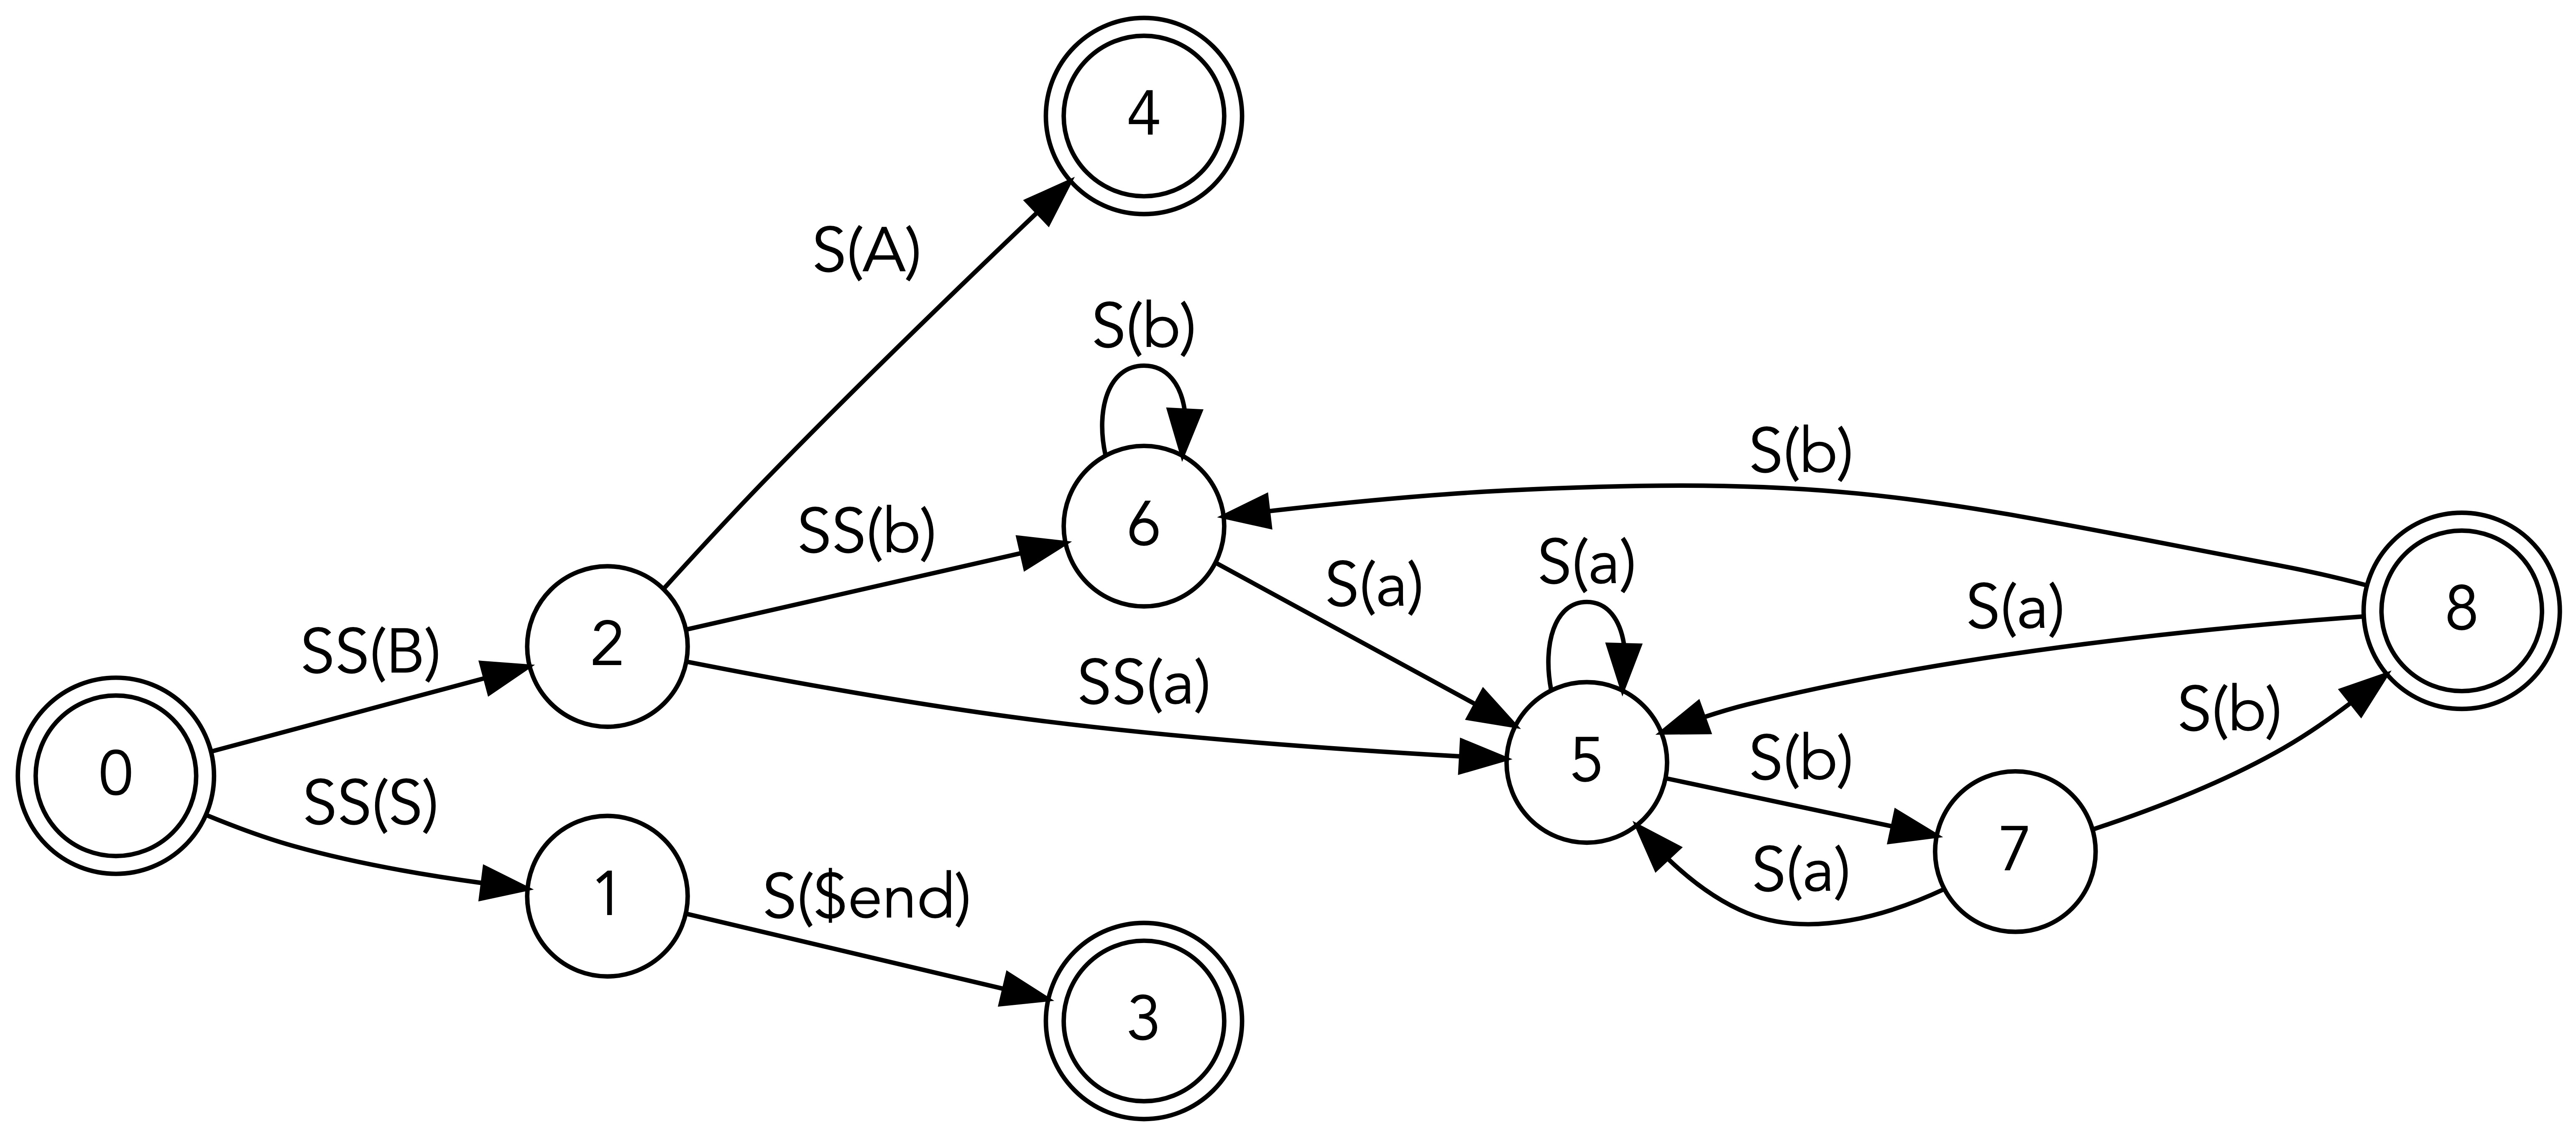
\includegraphics[width=5.5in,height=3.5in]{index_files/figure-latex/dot-figure-4.png}

}

\end{figure}

}

\caption{\label{fig-scriv17}\textbf{?(caption)}}

\end{figure}

\hypertarget{fig-scriv18}{}
\begin{figure*}

\begin{figure}[H]

{\centering 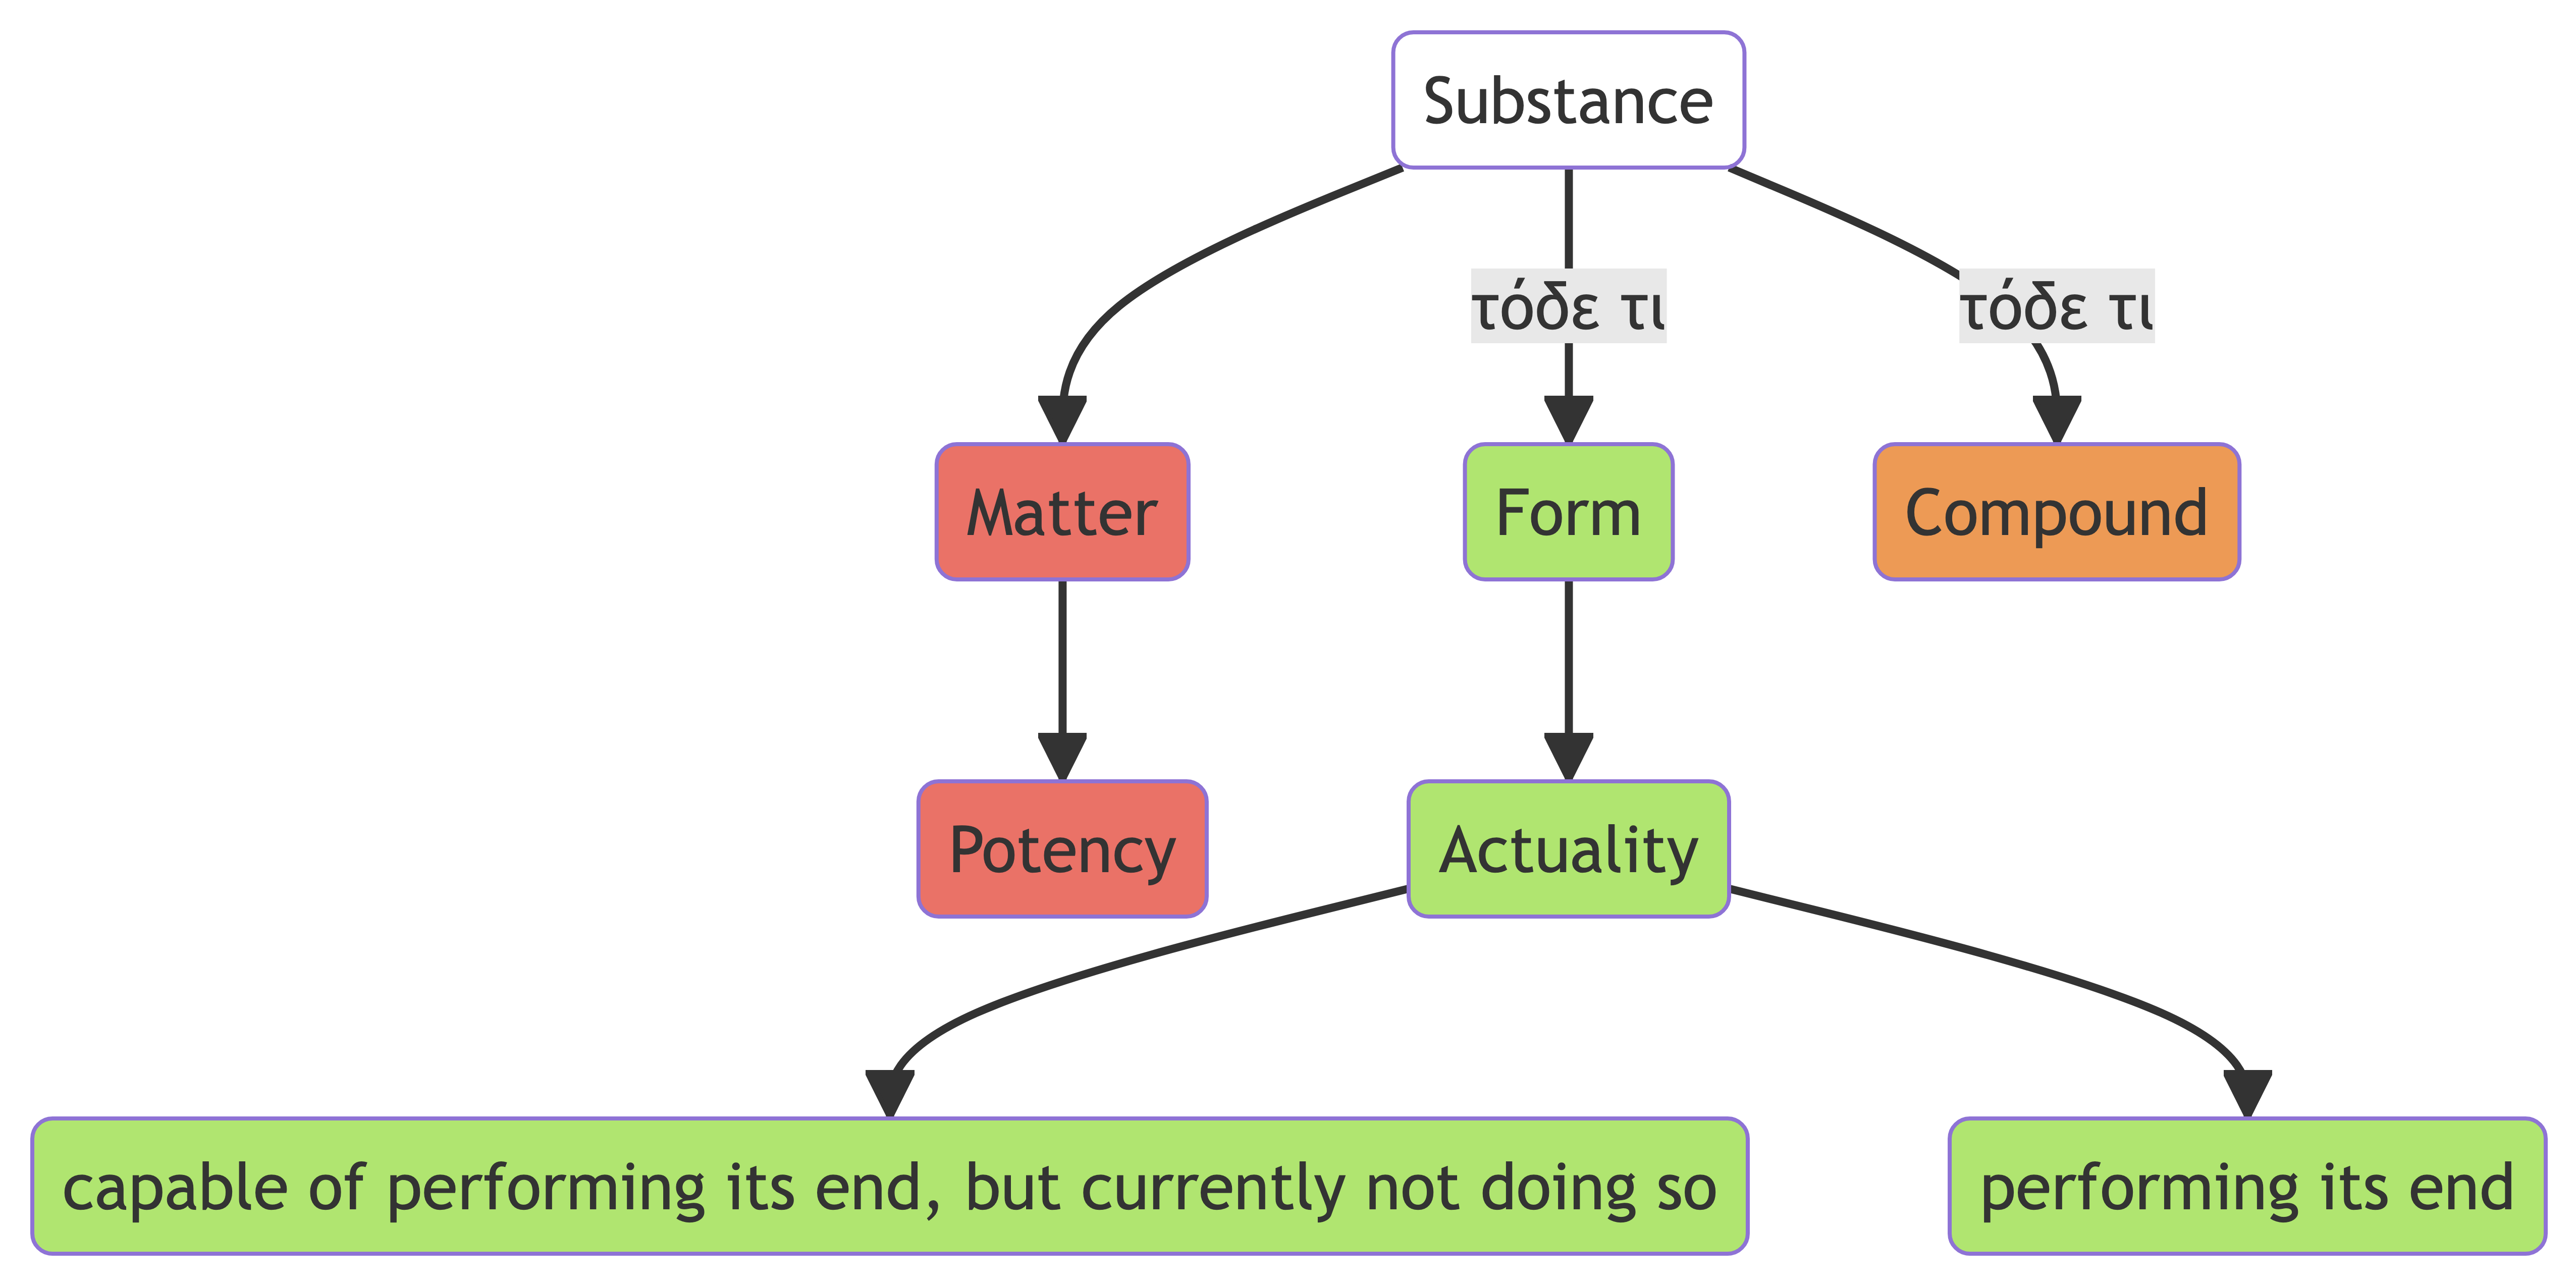
\includegraphics[width=17.26in,height=4.08in]{index_files/figure-latex/mermaid-figure-1.png}

}

\end{figure}

\label{fig-scriv18}Figure caption

\end{figure*}

\begin{figure}

{\centering 

\begin{figure}[H]

{\centering 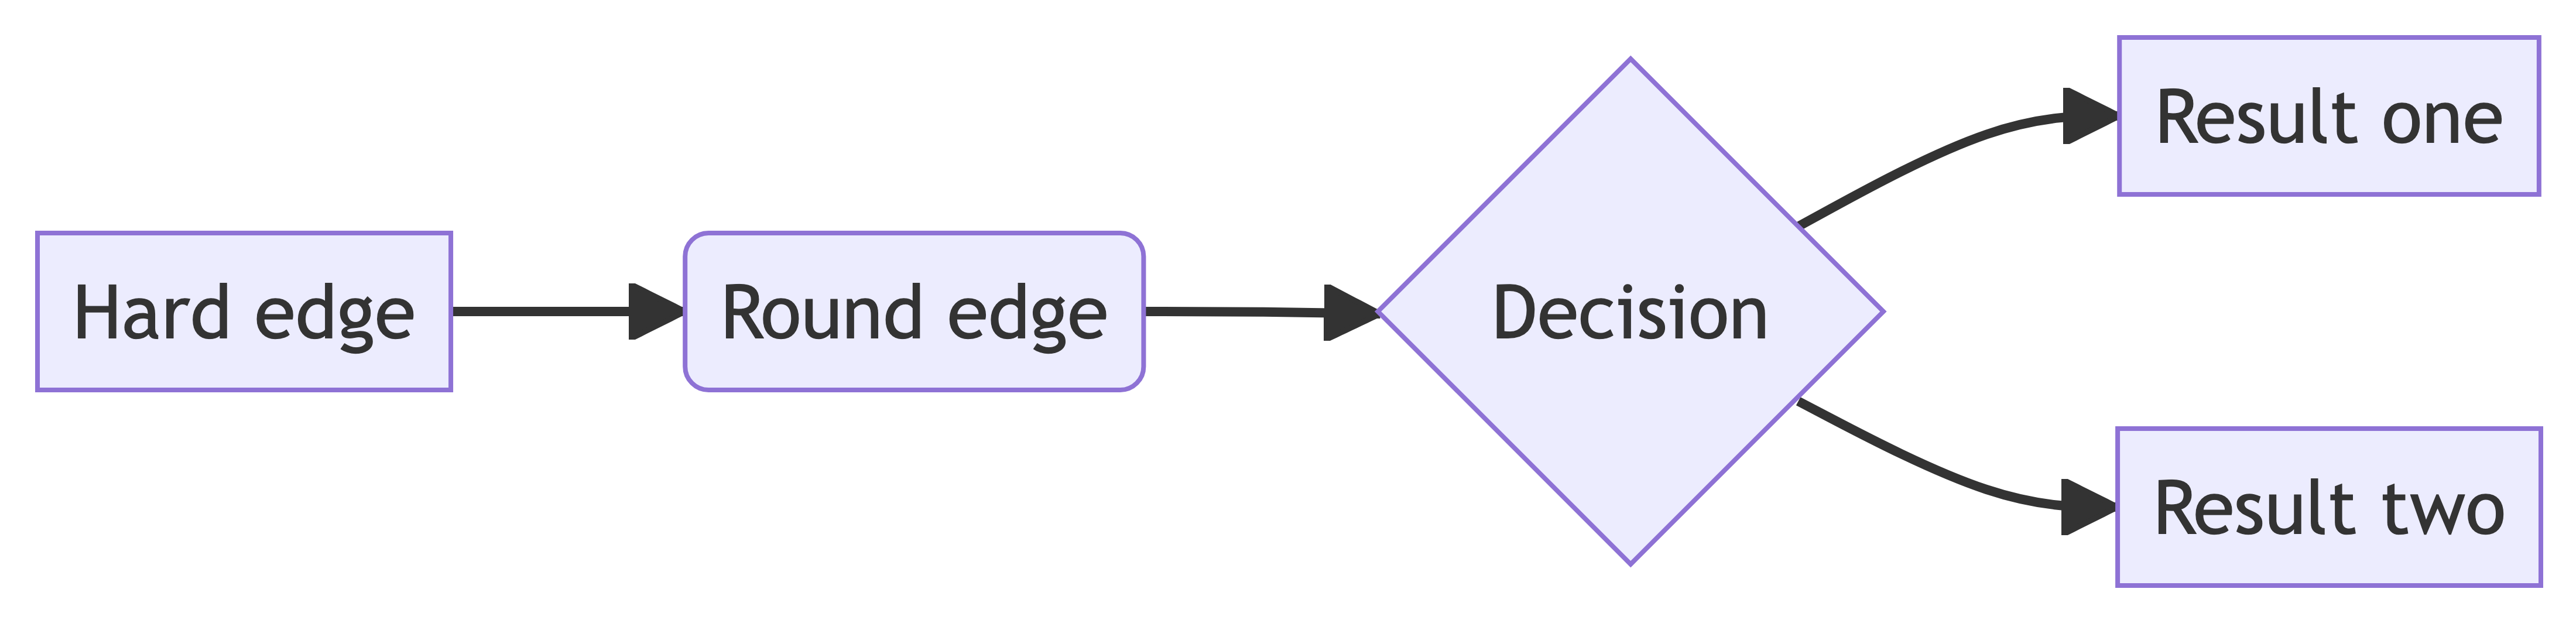
\includegraphics[width=5.73in,height=1.39in]{index_files/figure-latex/mermaid-figure-4.png}

}

\end{figure}

}

\caption{\label{fig-scriv18B}Figure caption}

\end{figure}

\begin{figure}

{\centering 

\begin{figure}[H]

{\centering 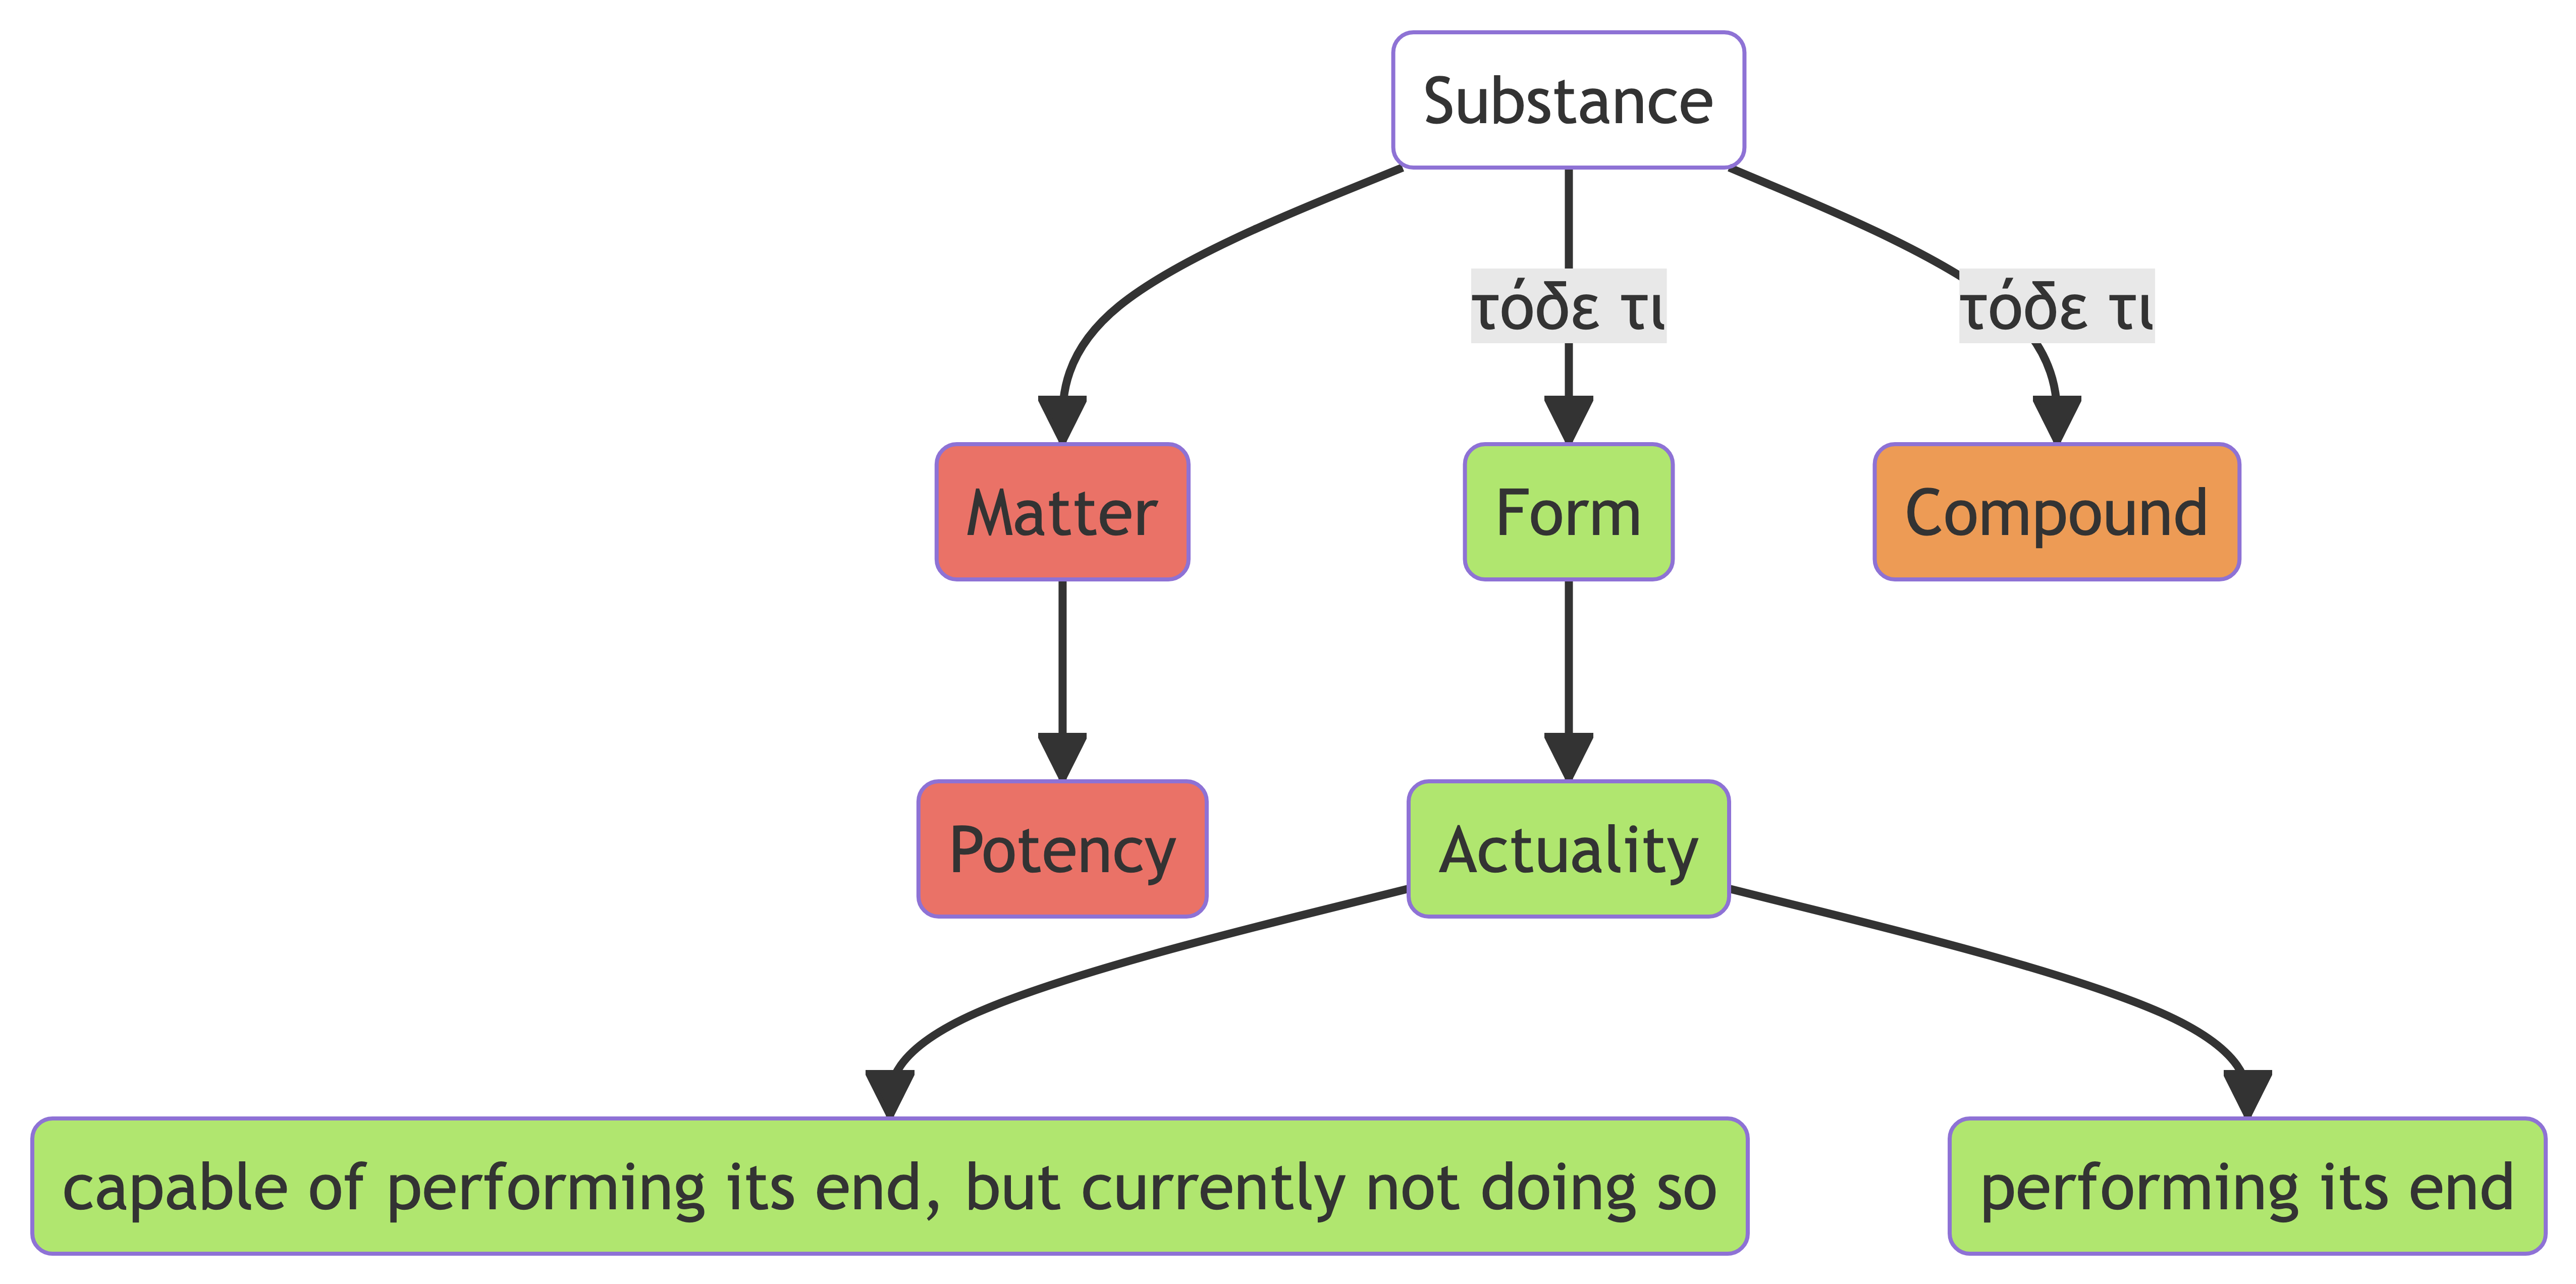
\includegraphics[width=6.65in,height=3.32in]{index_files/figure-latex/mermaid-figure-3.png}

}

\end{figure}

}

\caption{\label{fig-scriv19}\textbf{?(caption)}}

\end{figure}

\hypertarget{tbl-scriv20}{}
\begin{longtable}[]{@{}ccc@{}}
\toprule\noalign{}
\textbf{Element} & \textbf{Markdown Source} & \textbf{Rendered
Output} \\
\midrule\noalign{}
\endfirsthead
\toprule\noalign{}
\textbf{Element} & \textbf{Markdown Source} & \textbf{Rendered
Output} \\
\midrule\noalign{}
\endhead
\bottomrule\noalign{}
\endlastfoot
Equation & \texttt{{[}@eq-scriv21{]}} &
\protect\hypertarget{cite_56}{}{\label{cite_56}Equation~\ref{eq-scriv21}} \\
Equation & \texttt{{[}@eq-scriv22{]}} &
\protect\hypertarget{cite_57}{}{\label{cite_57}Equation~\ref{eq-scriv22}} \\
\caption{\label{tbl-scriv20}Cross-referencing
\textbf{Equations}.}\tabularnewline
\end{longtable}

\begin{equation}\protect\hypertarget{eq-scriv21}{}{t' = \frac{t - \dfrac{v}{c^{2}}x}{\sqrt{1 - \dfrac{v^{2}}{c^{2}}}}}\label{eq-scriv21}\end{equation}

\begin{equation}\protect\hypertarget{eq-scriv22}{}{t' = \frac{t - \dfrac{v}{c^{2}}x}{\sqrt{1 - \dfrac{v^{2}}{c^{2}}}}
}\label{eq-scriv22}\end{equation}

\hypertarget{sec-scriv23}{%
\subsection{Figures}\label{sec-scriv23}}

\protect\hypertarget{scriv23}{}{}

\hypertarget{tbl-scriv23}{}
\begin{longtable}[]{@{}ccc@{}}
\toprule\noalign{}
\textbf{Element} & \textbf{Markdown Source} & \textbf{Rendered
Output} \\
\midrule\noalign{}
\endfirsthead
\toprule\noalign{}
\textbf{Element} & \textbf{Markdown Source} & \textbf{Rendered
Output} \\
\midrule\noalign{}
\endhead
\bottomrule\noalign{}
\endlastfoot
Figure & \texttt{{[}@fig-scriv24{]}} &
\protect\hypertarget{cite_58}{}{\label{cite_58}Figure~\ref{fig-scriv24}} \\
Figure (Multipart) & \texttt{{[}@fig-scriv25{]}} &
\protect\hypertarget{cite_59}{}{\label{cite_59}Figure~\ref{fig-scriv25}} \\
Figure (Multipart) & \texttt{{[}@fig-scriv25A{]}} &
\protect\hypertarget{cite_60}{}{\label{cite_60}Figure~\ref{fig-scriv25A}} \\
Figure (Multipart) & \texttt{{[}@fig-scriv25B{]}} &
\protect\hypertarget{cite_61}{}{\label{cite_61}Figure~\ref{fig-scriv25B}} \\
Figure (Multipart) & \texttt{{[}@fig-scriv26{]}} &
\protect\hypertarget{cite_62}{}{\label{cite_62}Figure~\ref{fig-scriv26}} \\
Figure (Multipart) & \texttt{{[}@fig-scriv26A{]}} &
\protect\hypertarget{cite_63}{}{\label{cite_63}Figure~\ref{fig-scriv26A}} \\
Figure (Multipart) & \texttt{{[}@fig-scriv26B{]}} &
\protect\hypertarget{cite_64}{}{\label{cite_64}Figure~\ref{fig-scriv26B}} \\
\caption{\label{tbl-scriv23}Cross-referencing
\textbf{Figures}.}\tabularnewline
\end{longtable}

\begin{figure*}

{\centering 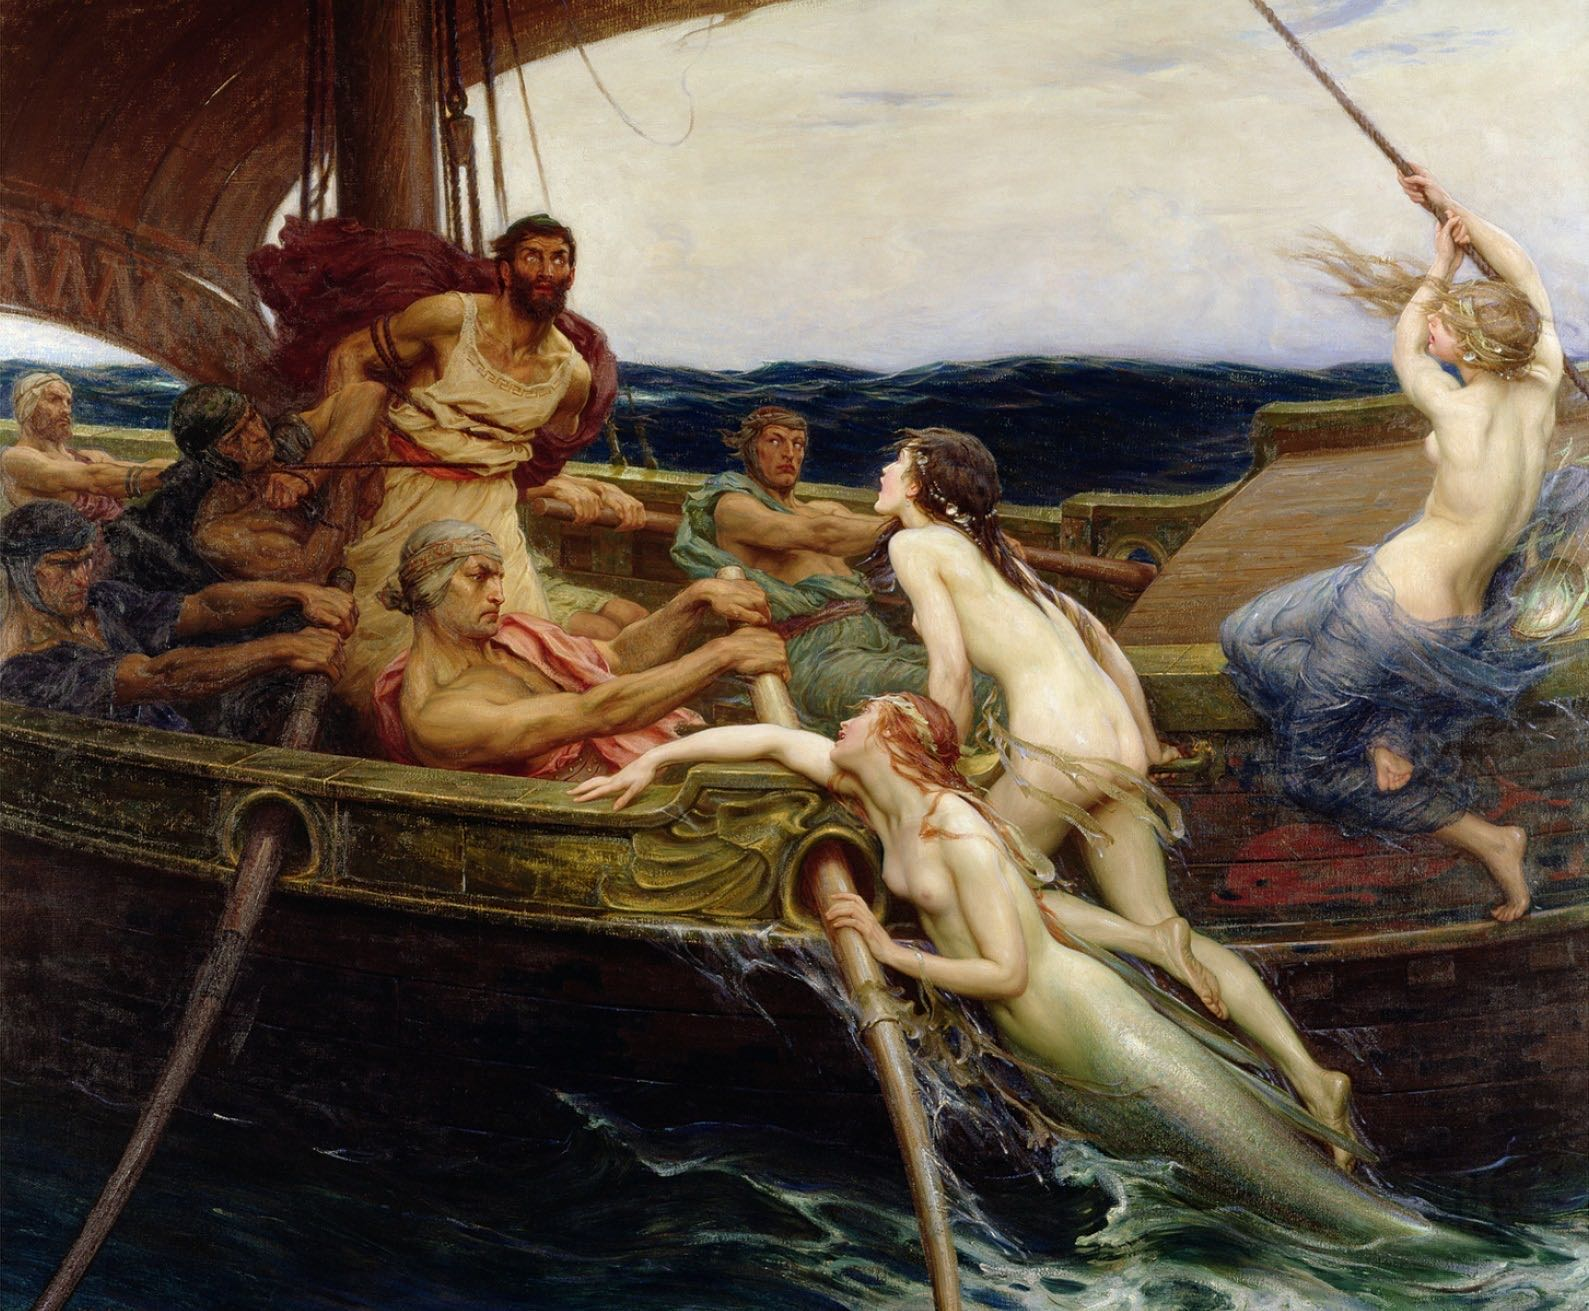
\includegraphics[width=5.0625in,height=4.1875in]{Ulysses1.jpg}

}

\caption{\label{fig-scriv24}This figure uses custom metadata values to
identify the class, ID, width and height. The \%CA\%\hspace{0pt}
(\textbf{C}aption \textbf{A}ttributes) tag at the start of the caption
is replaced with the correct Scrivener placeholders by the compiler; see
global replacements for the details\ldots{}}

\end{figure*}

\begin{figure*}

\begin{minipage}[t]{0.45\linewidth}

{\centering 

\raisebox{-\height}{

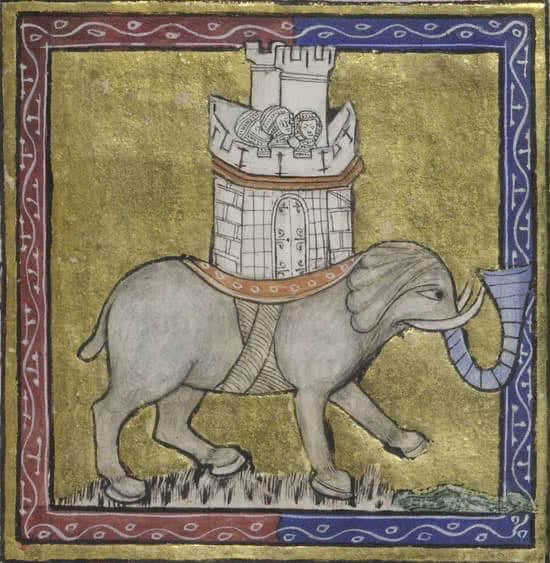
\includegraphics[width=2.55208in,height=\textheight]{Elephant2.jpg}

}

}

\subcaption{\label{fig-scriv25A}Elephant.}
\end{minipage}%
%
\begin{minipage}[t]{0.56\linewidth}

{\centering 

\raisebox{-\height}{

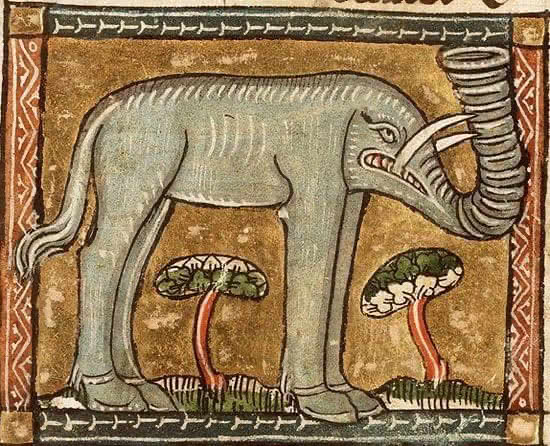
\includegraphics[width=3.1875in,height=\textheight]{Elephant3.jpg}

}

}

\subcaption{\label{fig-scriv25B}Angry elephant with a big trunk.}
\end{minipage}%

\caption{\label{fig-scriv25}This demonstrates generating a multi-panel
figure using a Scrivener Section Type {[}\texttt{Multipart\ Figure}{]}
instead of using raw markdown as shown here. ID, Class, and Attributes
specific to the block
{[}\texttt{\#fig-elephants2\ .column-body\ layout-ncol=2\ layout-valign="bottom"}{]}
are saved to
\texttt{Custom\ Metadata-\textgreater{}ID,\ Class\ \&\ Attributes}, and
this is then inserted into the markup for this chunk by the Section
Layout at compile time.}

\end{figure*}

\begin{figure*}

\begin{minipage}[t]{0.44\linewidth}

{\centering 

\raisebox{-\height}{

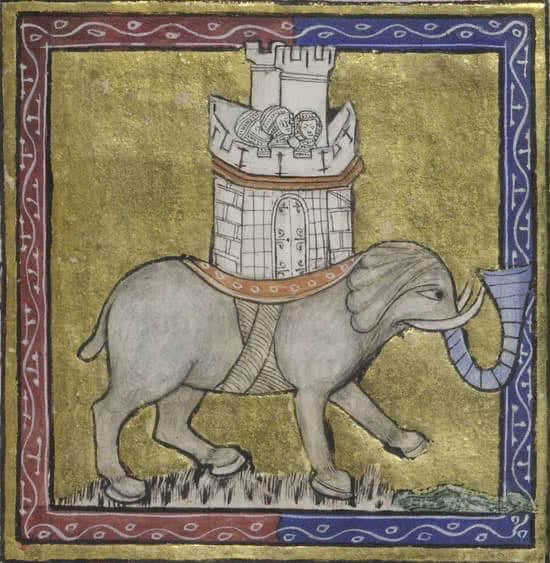
\includegraphics[width=2.53125in,height=\textheight]{Elephant2.jpg}

}

}

\subcaption{\label{fig-scriv26A}Elephant castle.}
\end{minipage}%
%
\begin{minipage}[t]{0.56\linewidth}

{\centering 

\raisebox{-\height}{

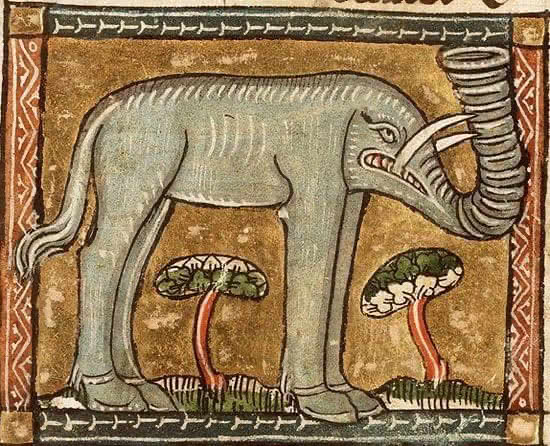
\includegraphics[width=3.16667in,height=\textheight]{Elephant3.jpg}

}

}

\subcaption{\label{fig-scriv26B}Angry elephant with a big trunk.}
\end{minipage}%

\caption{\label{fig-scriv26}Quarto allows the creation of figure panels
with sub-figures. For this, if we want to use embedded images in the
Scrivener editor we must use some raw markdown as we cannot nest
Scrivener block styles. Note we can use the Scale Image\ldots{} Tool in
Scrivener and these sizes get exported to Quarto and the output. Here we
scale both images to the same height.}

\end{figure*}

\hypertarget{sec-scriv27}{%
\subsection{Listings}\label{sec-scriv27}}

\protect\hypertarget{scriv27}{}{}

\hypertarget{tbl-scriv27}{}
\begin{longtable}[]{@{}ccc@{}}
\toprule\noalign{}
\textbf{Element} & \textbf{Markdown Source} & \textbf{Rendered
Output} \\
\midrule\noalign{}
\endfirsthead
\toprule\noalign{}
\textbf{Element} & \textbf{Markdown Source} & \textbf{Rendered
Output} \\
\midrule\noalign{}
\endhead
\bottomrule\noalign{}
\endlastfoot
Listing & \texttt{{[}@lst-scriv28{]}} &
\protect\hypertarget{cite_65}{}{\label{cite_65}Listing~\ref{lst-scriv28}} \\
Listing & \texttt{{[}@lst-scriv29{]}} &
\protect\hypertarget{cite_66}{}{\label{cite_66}Listing~\ref{lst-scriv29}} \\
\caption{\label{tbl-scriv27}Cross-referencing
\textbf{Listings}.}\tabularnewline
\end{longtable}

\begin{codelisting}

\caption{Ruby code block. The listing Paragraph Style uses the custom
metadata of the current text document.}

\hypertarget{lst-scriv28}{%
\label{lst-scriv28}}%
\begin{Shaded}
\begin{Highlighting}[numbers=left,,]
\FunctionTok{require} \StringTok{"unicode/name"}

\NormalTok{characters }\KeywordTok{=}\OtherTok{ \%w(}\StringTok{α β γ δ ε ζ η θ ι κ λ μ ν ξ ο π ρ σ τ υ φ χ ψ ω ἀ ἄ ᾄ ἂ ᾂ ἆ ᾆ ᾀ ἁ ἅ ᾅ ἃ ᾃ ἇ ᾇ ᾁ ά ά ᾴ ὰ ᾲ ᾰ ᾶ ᾷ ᾱ ᾳ ἐ ἔ ἒ ἑ ἕ ἓ έ έ ὲ}\OtherTok{)}

\CommentTok{\# characters = \textquotesingle{}ἄ\textquotesingle{}}
\NormalTok{characters}\AttributeTok{.each} \ControlFlowTok{do} \KeywordTok{|}\NormalTok{character}\KeywordTok{|}
  \FunctionTok{puts}\NormalTok{ character}\AttributeTok{.unpack}\NormalTok{(}\VerbatimStringTok{\textquotesingle{}U*\textquotesingle{}}\NormalTok{)}\AttributeTok{.map} \KeywordTok{\{} \KeywordTok{|}\NormalTok{i}\KeywordTok{|} \StringTok{"U+}\SpecialCharTok{\#\{}\NormalTok{i}\AttributeTok{.to\_s}\NormalTok{(}\DecValTok{16}\NormalTok{)}\AttributeTok{.rjust}\NormalTok{(}\DecValTok{4}\NormalTok{, }\CharTok{\textquotesingle{}0\textquotesingle{}}\NormalTok{)}\AttributeTok{.upcase}\SpecialCharTok{\}}\StringTok{"} \KeywordTok{\}}\AttributeTok{.join}
  \FunctionTok{puts} \DataTypeTok{Unicode}\KeywordTok{::}\DataTypeTok{Name}\AttributeTok{.of}\NormalTok{ character}
\ControlFlowTok{end}
\end{Highlighting}
\end{Shaded}

\end{codelisting}

\begin{codelisting}

\caption{The caption}

\hypertarget{lst-scriv29}{%
\label{lst-scriv29}}%
\begin{Shaded}
\begin{Highlighting}[numbers=left,,]

\ControlFlowTok{\#!/usr/bin/env ruby}
\CommentTok{\# frozen\_string\_literal: false}

\DataTypeTok{Encoding}\AttributeTok{.default\_external} \KeywordTok{=} \DataTypeTok{Encoding}\KeywordTok{::}\DataTypeTok{UTF\_8}

\DataTypeTok{Dir}\KeywordTok{[}\StringTok{"}\SpecialCharTok{\#\{}\NormalTok{\_\_dir\_\_}\SpecialCharTok{\}}\StringTok{/Ruby/**/*.rb"}\KeywordTok{]}\AttributeTok{.each} \ControlFlowTok{do} \KeywordTok{|}\NormalTok{file}\KeywordTok{|}
  \FunctionTok{require\_relative}\NormalTok{ file}
\ControlFlowTok{end}
\end{Highlighting}
\end{Shaded}

\end{codelisting}

\hypertarget{sec-scriv30}{%
\subsection{Tables}\label{sec-scriv30}}

\protect\hypertarget{scriv30}{}{}

\hypertarget{tbl-scriv30}{}
\begin{longtable}[]{@{}ccc@{}}
\toprule\noalign{}
\textbf{Element} & \textbf{Markdown Source} & \textbf{Rendered
Output} \\
\midrule\noalign{}
\endfirsthead
\toprule\noalign{}
\textbf{Element} & \textbf{Markdown Source} & \textbf{Rendered
Output} \\
\midrule\noalign{}
\endhead
\bottomrule\noalign{}
\endlastfoot
Table & \texttt{{[}@tbl-scriv31{]}} &
\protect\hypertarget{cite_67}{}{\label{cite_67}Table~\ref{tbl-scriv31}} \\
Table & \texttt{{[}@tbl-scriv32{]}} &
\protect\hypertarget{cite_68}{}{\label{cite_68}Table~\ref{tbl-scriv32}} \\
Table (Multipart) & \texttt{{[}@tbl-scriv33{]}} &
\protect\hypertarget{cite_69}{}{\label{cite_69}Table~\ref{tbl-scriv33}} \\
Table (Multipart) & \texttt{{[}@tbl-scriv33A{]}} &
\protect\hypertarget{cite_70}{}{\label{cite_70}Table~\ref{tbl-scriv33A}} \\
Table (Multipart) & \texttt{{[}@tbl-scriv33B{]}} &
\protect\hypertarget{cite_71}{}{\label{cite_71}Table~\ref{tbl-scriv33B}} \\
\caption{\label{tbl-scriv30}Cross-referencing
\textbf{Tables}.}\tabularnewline
\end{longtable}

\hypertarget{tbl-scriv31}{}
\begin{longtable}[]{@{}lll@{}}
\toprule\noalign{}
1 & 2 & 3 \\
\midrule\noalign{}
\endfirsthead
\toprule\noalign{}
1 & 2 & 3 \\
\midrule\noalign{}
\endhead
\bottomrule\noalign{}
\endlastfoot
4 & 5 & 6 \\
\caption{\label{tbl-scriv31}This table uses \texttt{Text} as the
\textbf{Section Type}, and \texttt{Table\ Caption} as the
\textbf{Paragraph Style} for the caption.}\tabularnewline
\end{longtable}

\hypertarget{tbl-scriv32}{}
\begin{longtable}[]{@{}lll@{}}
\toprule\noalign{}
1 & 2 & 3 \\
\midrule\noalign{}
\endfirsthead
\toprule\noalign{}
1 & 2 & 3 \\
\midrule\noalign{}
\endhead
\bottomrule\noalign{}
\endlastfoot
4 & 5 & 6 \\
\caption{\label{tbl-scriv32}This is an example of \texttt{Table} as
\textbf{Section Type}. The caption and the remaining attributes are
added as part of the Section Type markup.}\tabularnewline
\end{longtable}

\begin{table}

\begin{minipage}[t]{\linewidth}

{\centering 

\begin{tabular}[t]{cccc}
\toprule
\textbf{Element} & \textbf{Prefix} & \textbf{Markdown
Source} & \textbf{Rendered Output}\\
\midrule
Equation A & eq & A & B\\
Equation A & eq & C & D\\
Listing A & lst & E & F\\
\bottomrule
\end{tabular}

}

\subcaption{\label{tbl-scriv33A}First Table}
\end{minipage}%
\newline
\begin{minipage}[t]{\linewidth}

{\centering 

\begin{tabular}[t]{cccc}
\toprule
\textbf{Element} & \textbf{Prefix} & \textbf{Markdown
Source} & \textbf{Rendered Output}\\
\midrule
Equation B & eq & A & B\\
Equation B & eq & C & D\\
Listing B & lst & E & F\\
\bottomrule
\end{tabular}

}

\subcaption{\label{tbl-scriv33B}Second Table}
\end{minipage}%

\caption{\label{tbl-scriv33}This is a markdown multi-table panel with
two sub-tables generated using a Section Type
{[}\texttt{Multipart\ Table}{]}. Note that Custom Metadata holds the
cross-referencing label, layout class, and the attributes for this
multipart table, which will be added by the Section Layout by the
compiler, using the Scrivener placeholders:
\texttt{\textless{}\hspace{0pt}\$\hspace{0pt}\hspace{0pt}custom:Class\textgreater{}}
\texttt{\textless{}\hspace{0pt}\$\hspace{0pt}\hspace{0pt}custom:Attributes\textgreater{}}}

\end{table}

\hypertarget{sec-scriv34}{%
\subsection{Sections}\label{sec-scriv34}}

\protect\hypertarget{scriv34}{}{}

The text sections can be referenced with \textbf{Character Styles}, and
created with \textbf{Paragraph Styles} or \textbf{Section Types}. As
before, all of these receive automatic IDs.

\hypertarget{tbl-scriv34}{}
\begin{longtable}[]{@{}ccc@{}}
\toprule\noalign{}
\textbf{Element} & \textbf{Markdown Source} & \textbf{Rendered
Output} \\
\midrule\noalign{}
\endfirsthead
\toprule\noalign{}
\textbf{Element} & \textbf{Markdown Source} & \textbf{Rendered
Output} \\
\midrule\noalign{}
\endhead
\bottomrule\noalign{}
\endlastfoot
Section & \texttt{{[}@sec-scriv34{]}} &
\protect\hypertarget{cite_72}{}{\label{cite_72}Section~\ref{sec-scriv34}} \\
Section & \texttt{{[}@sec-scriv35{]}} &
\protect\hypertarget{cite_73}{}{\label{cite_73}Section~\ref{sec-scriv35}} \\
Section & \texttt{{[}@sec-scriv37{]}} &
\protect\hypertarget{cite_74}{}{\label{cite_74}Section~\ref{sec-scriv37}} \\
Section & \texttt{{[}@sec-scriv38{]}} &
\protect\hypertarget{cite_75}{}{\label{cite_75}Section~\ref{sec-scriv38}} \\
Section & \texttt{{[}@sec-scriv39{]}} &
\protect\hypertarget{cite_76}{}{\label{cite_76}Section~\ref{sec-scriv39}} \\
\caption{\label{tbl-scriv34}Cross-referencing sections.}\tabularnewline
\end{longtable}

Note that the unnumbered section cannot be referenced.

\hypertarget{sec-scriv35}{%
\subsubsection{Section}\label{sec-scriv35}}

\protect\hypertarget{scriv35}{}{}

This is an example of the \texttt{Section} section type.

\hypertarget{sec-scriv36}{%
\subsubsection*{Section \{-\}}\label{sec-scriv36}}
\addcontentsline{toc}{subsubsection}{Section \{-\}}

\protect\hypertarget{scriv36}{}{}

This is an example of the \texttt{Section\ \{-\}} section type.

\hypertarget{sec-scriv37}{%
\subsubsection{Heading}\label{sec-scriv37}}

\hypertarget{sec-scriv38}{%
\subsubsection{Heading + Break}\label{sec-scriv38}}

This is an example of the \texttt{Heading\ +\ Break} section type.

\newpage{}

\newpage{}

\hypertarget{sec-scriv39}{%
\subsubsection{Section + Break}\label{sec-scriv39}}

This is an example of the \texttt{Section\ +\ Break} section type.

\hypertarget{sec-scriv40}{%
\section{Footnotes}\label{sec-scriv40}}

\protect\hypertarget{scriv40}{}{}

We can use also use a \textbf{Section Type} to create and a
\textbf{Character Style} (\texttt{Footnote}) to reference footnotes
using the standard identifier.\footnote{\protect\hypertarget{scriv41}{}{}
  This strategy has the outstanding advantage of allowing us to use,
  that is right, you guessed it, \textbf{Paragraph Styles} and
  \textbf{Character Styles} in footnotes. There is one small caveat,
  however: the user has to remember to \ul{always add two empty spaces}
  before each new \textbf{paragraph} in the footnote environment.}

\hypertarget{sec-scriv42}{%
\chapter{Cite Tools}\label{sec-scriv42}}

\protect\hypertarget{scriv42}{}{}

Part of the motivation behind ScrivQ comes from another project I
co-developed: the
\href{https://bcdavasconcelos.github.io/citetools}{Cite Tools} extension
for \href{https://pandoc.org}{Pandoc} and
\href{https://quarto.org}{Quarto}.

As I was first starting to use
\href{https://en.wikipedia.org/wiki/CiteProc}{Citeproc}, coming from the
jurassic
\textbf{\href{https://en.wikipedia.org/wiki/BibTeX\#Entry_types}{BibTeX}},
I was exceptionally pleased with its speed and reliability. Apart from
being \emph{a lot} faster, it would produce the same output across all
supported formats (which amounts to over 60). Out-of-the-box, however,
it lacked support for really ordinary \textbf{BibTeX functionalities},
such as the ability to split the bibliography into multiple sections, or
the ability to cite arbitrary fields of the references (\emph{e.g.}
using \texttt{citetitle}, \texttt{citeauthor}, \texttt{citefield}). It
also lacked the interesting \textbf{backref} option afforded by
\textbf{BibTeX} used in conjunction with \textbf{HyperRef} to create
linked indexes of citations.

\begin{figure}

{\centering 
\includegraphics[width=2.875in,height=2.875in]{citetools.png}

}

\caption{\label{fig-scriv42}Cite Tool bundles together several lua
filters to address complex bibliography demands while keeping the output
consistent across formats. If you have suggestions for improvements or
bug reports, please
\href{https://github.com/bcdavasconcelos/citetools/issues/new/choose}{open
an issue at the citetools repository}. Logo image generated with Dall-E
using \enquote{\emph{Enso-like round black and white painting with
ancient greek war-ship with a man tied to the mast as prompt}}.}

\end{figure}

To step around these limitations, I started tinkering with existing
filters available on GitHub (all of them by Albert Krewinkel), and
co-developed Cite Field, to create \textbf{Cite Tools}, an extension for
Quarto and Pandoc that allows the easy creation of a \textbf{Multipart
Bibliography} (\emph{e.g.} split in \emph{primary} and \emph{secondary}
sources, see
\protect\hypertarget{cite_77}{}{\label{cite_77}Figure~\ref{fig-scriv54A}}),
the citation of arbitrary fields of the references (see
\protect\hypertarget{cite_78}{}{\label{cite_78}Figure~\ref{fig-scriv54B}})\footnote{In
  the official nomenclature, CSL has variables, BibTeX has fields, and
  RIS has tags. As a general rule, we have stuck to the term fields.},
and the linking of each bibliography entry back to its in-text
occurrences (see
\protect\hypertarget{cite_79}{}{\label{cite_79}Figure~\ref{fig-scriv54C}})\footnote{Linked
  glossaries can also easily be created by dressing them as
  bibliography.}. The filters are built-in, and the front matter is set
up so that the necessary files are automatically created during
compilation.

\begin{tcolorbox}[enhanced jigsaw, left=2mm, colframe=quarto-callout-warning-color-frame, colback=white, opacityback=0, breakable, toprule=.15mm, arc=.35mm, rightrule=.15mm, bottomrule=.15mm, leftrule=.75mm]
\begin{minipage}[t]{5.5mm}
\textcolor{quarto-callout-warning-color}{\faExclamationTriangle}
\end{minipage}%
\begin{minipage}[t]{\textwidth - 5.5mm}

\textbf{Deleting Cite Tools from ScrivQ \ul{will cause the compilation
to fail}.}\vspace{2mm}

\end{minipage}%
\end{tcolorbox}

\begin{tcolorbox}[enhanced jigsaw, left=2mm, colframe=quarto-callout-tip-color-frame, colback=white, opacityback=0, breakable, toprule=.15mm, arc=.35mm, rightrule=.15mm, bottomrule=.15mm, leftrule=.75mm]
\begin{minipage}[t]{5.5mm}
\textcolor{quarto-callout-tip-color}{\faLightbulb}
\end{minipage}%
\begin{minipage}[t]{\textwidth - 5.5mm}

If you need to use \textbf{Cite Tools }in an ordinary Quarto project,
use \texttt{quarto\ install\ extension\ bcdavasconcelos/citetools} to
install it.

\end{minipage}%
\end{tcolorbox}

\hypertarget{sec-scriv43}{%
\section{Citation}\label{sec-scriv43}}

\protect\hypertarget{scriv43}{}{}

Let us quickly recapitulate the basics of Pandoc Citeproc and how it
uses citations.

\begin{tcolorbox}[enhanced jigsaw, left=2mm, colframe=quarto-callout-note-color-frame, bottomtitle=1mm, colback=white, coltitle=black, title=\textcolor{quarto-callout-note-color}{\faInfo}\hspace{0.5em}{Official documentation}, toprule=.15mm, rightrule=.15mm, opacityback=0, breakable, toptitle=1mm, titlerule=0mm, colbacktitle=quarto-callout-note-color!10!white, arc=.35mm, bottomrule=.15mm, leftrule=.75mm, opacitybacktitle=0.6]

See the official documentation on citations at
\href{pandoc.org/MANUAL.html\#citations}{Pandoc} and
\href{quarto.org/docs/authoring/footnotes-and-citations.html\#sec-citations}{Quarto}.

\end{tcolorbox}

\marginnote{\begin{footnotesize}

As we know, each citation must have a key, composed of \texttt{@} + the
citation identifier that must begin with a letter, digit, or
\texttt{\_}, and may contain alphanumerics, \texttt{\_}, and internal
punctuation characters
(\texttt{:.\#\$\%\&-+?\textless{}\textgreater{}\textasciitilde{}/}).

\end{footnotesize}}

The citation syntax is very simple: \texttt{@Citekey} for \textbf{Author
(Date)} (an \emph{in-text} citation); \texttt{{[}@Citekey{]}} for
\textbf{(Author, Date)}; and \texttt{{[}-@Citekey{]}} for
\textbf{(Date)}. Multiple citations can be grouped in the same brackets
separated by semicolons \texttt{{[}@CitekeyA;\ @CitekeyB{]}}. The
citation key is optionally followed by a locator, which can be a page
number, a line number, a chapter number, or a section number, preceded
by a comma.

\hypertarget{tbl-scriv43}{}
\begin{longtable}[]{@{}cc@{}}
\toprule\noalign{}
\textbf{Markdown Source} & \textbf{Rendered output} \\
\midrule\noalign{}
\endfirsthead
\toprule\noalign{}
\textbf{Markdown Source} & \textbf{Rendered output} \\
\midrule\noalign{}
\endhead
\bottomrule\noalign{}
\endlastfoot
\texttt{@Long2004} & \protect\hypertarget{cite_80}{}{\label{cite_80}Long
(\protect\hyperlink{ref-Long2004}{2004})} \\
\texttt{{[}@Long2004{]}} &
\protect\hypertarget{cite_81}{}{\label{cite_81}(\protect\hyperlink{ref-Long2004}{Long
2004})} \\
\texttt{{[}@Long2004,\ p.15{]}} &
\protect\hypertarget{cite_82}{}{\label{cite_82}(\protect\hyperlink{ref-Long2004}{Long
2004, 15})} \\
\texttt{{[}-@Long2004{]}} &
\protect\hypertarget{cite_83}{}{\label{cite_83}(\protect\hyperlink{ref-Long2004}{2004})} \\
\texttt{{[}-@Long2004,\ p.15{]}} &
\protect\hypertarget{cite_84}{}{\label{cite_84}(\protect\hyperlink{ref-Long2004}{2004,
15})} \\
\caption{\label{tbl-scriv43}Citation syntax in Quarto and
Pandoc.}\tabularnewline
\end{longtable}

\begin{tcolorbox}[enhanced jigsaw, left=2mm, colframe=quarto-callout-note-color-frame, colback=white, opacityback=0, breakable, toprule=.15mm, arc=.35mm, rightrule=.15mm, bottomrule=.15mm, leftrule=.75mm]
\begin{minipage}[t]{5.5mm}
\textcolor{quarto-callout-note-color}{\faInfo}
\end{minipage}%
\begin{minipage}[t]{\textwidth - 5.5mm}

\textbf{(Date)}\vspace{2mm}

\ldots on the deliberations of the prudent person
\protect\hypertarget{cite_85}{}{\label{cite_85}(\protect\hyperlink{ref-Long2004}{2004})}.
\texttt{...on\ the\ deliberations\ of\ the\ prudent\ person\ {[}-@Long2004{]}.}

\ldots on the deliberations of the prudent person
\protect\hypertarget{cite_86}{}{\label{cite_86}(\protect\hyperlink{ref-Long2004}{2004,
17})}.
\texttt{...on\ the\ deliberations\ of\ the\ prudent\ person\ {[}-@Long2004,\ p.17{]}.}

\end{minipage}%
\end{tcolorbox}

\begin{tcolorbox}[enhanced jigsaw, left=2mm, colframe=quarto-callout-note-color-frame, colback=white, opacityback=0, breakable, toprule=.15mm, arc=.35mm, rightrule=.15mm, bottomrule=.15mm, leftrule=.75mm]
\begin{minipage}[t]{5.5mm}
\textcolor{quarto-callout-note-color}{\faInfo}
\end{minipage}%
\begin{minipage}[t]{\textwidth - 5.5mm}

\textbf{Author (Date)}\vspace{2mm}

\protect\hypertarget{cite_87}{}{\label{cite_87}Long
(\protect\hyperlink{ref-Long2004}{2004})} says that\ldots{}
\texttt{@Long2004\ says\ that...}

\end{minipage}%
\end{tcolorbox}

\begin{tcolorbox}[enhanced jigsaw, left=2mm, colframe=quarto-callout-note-color-frame, colback=white, opacityback=0, breakable, toprule=.15mm, arc=.35mm, rightrule=.15mm, bottomrule=.15mm, leftrule=.75mm]
\begin{minipage}[t]{5.5mm}
\textcolor{quarto-callout-note-color}{\faInfo}
\end{minipage}%
\begin{minipage}[t]{\textwidth - 5.5mm}

\textbf{(Author, Date)}\vspace{2mm}

\ldots on the deliberations of the prudent person
\protect\hypertarget{cite_88}{}{\label{cite_88}(\protect\hyperlink{ref-Long2004}{Long
2004})}.
\texttt{...on\ the\ deliberations\ of\ the\ prudent\ person\ {[}@Long2004{]}}.

\ldots on the deliberations of the prudent person
\protect\hypertarget{cite_89}{}{\label{cite_89}(\protect\hyperlink{ref-Long2004}{Long
2004, 17})}.
\texttt{...on\ the\ deliberations\ of\ the\ prudent\ person\ {[}@Long2004,\ p.17{]}}.

\end{minipage}%
\end{tcolorbox}

\begin{tcolorbox}[enhanced jigsaw, left=2mm, colframe=quarto-callout-note-color-frame, colback=white, opacityback=0, breakable, toprule=.15mm, arc=.35mm, rightrule=.15mm, bottomrule=.15mm, leftrule=.75mm]
\begin{minipage}[t]{5.5mm}
\textcolor{quarto-callout-note-color}{\faInfo}
\end{minipage}%
\begin{minipage}[t]{\textwidth - 5.5mm}

\textbf{(Author, Date; Author, Date)}\vspace{2mm}

\ldots on the deliberations of the prudent person
\protect\hypertarget{cite_90}{}{\label{cite_90}(\protect\hyperlink{ref-Long2004}{Long
2004}; \protect\hyperlink{ref-hoffman2014}{Hoffman and Prakash 2014})}.
\texttt{...on\ the\ deliberations\ of\ the\ prudent\ person\ {[}@Long2004;\ @hoffman2014{]}}.

\ldots on the deliberations of the prudent person
\protect\hypertarget{cite_91}{}{\label{cite_91}(\protect\hyperlink{ref-Long2004}{Long
2004, 17}; \protect\hyperlink{ref-hoffman2014}{Hoffman and Prakash 2014,
15})}.
\texttt{...on\ the\ deliberations\ of\ the\ prudent\ person\ {[}@Long2004,\ p.17;\ @hoffman2014,\ p.15{]}.}

\end{minipage}%
\end{tcolorbox}

That is pretty much all there is to it. Now that we have the basics
covered, let us see what \textbf{Cite Field} can do for us.

\hypertarget{sec-scriv44}{%
\section{Cite Field}\label{sec-scriv44}}

\protect\hypertarget{scriv44}{}{}

In many areas, we are frequently invited to comment on different
editions and translations of the same classical works. In such cases, we
refer not only to the \texttt{author} and the date \texttt{issued} of a
publication, but also to its \texttt{editor}, \texttt{translator},
\texttt{publisher}, and even \texttt{original-title} and
\texttt{edition}. But how to do this? With \textbf{Cite Tools} enabled,
the answer lies in a small variation of Pandoc's vanilla syntax for
citations.

\begin{tcolorbox}[enhanced jigsaw, left=2mm, colframe=quarto-callout-note-color-frame, bottomtitle=1mm, colback=white, coltitle=black, title=\textcolor{quarto-callout-note-color}{\faInfo}\hspace{0.5em}{TLDR}, toprule=.15mm, rightrule=.15mm, opacityback=0, breakable, toptitle=1mm, titlerule=0mm, colbacktitle=quarto-callout-note-color!10!white, arc=.35mm, bottomrule=.15mm, leftrule=.75mm, opacitybacktitle=0.6]

Several \textbf{Character Styles} are available to inject the correct
markup (\texttt{{[}@Citekey{]}\{.csl\_field\}}) to cite specific fields
from your references.

\end{tcolorbox}

\begin{tcolorbox}[enhanced jigsaw, left=2mm, colframe=quarto-callout-important-color-frame, bottomtitle=1mm, colback=white, coltitle=black, title=\textcolor{quarto-callout-important-color}{\faExclamation}\hspace{0.5em}{Important}, toprule=.15mm, rightrule=.15mm, opacityback=0, breakable, toptitle=1mm, titlerule=0mm, colbacktitle=quarto-callout-important-color!10!white, arc=.35mm, bottomrule=.15mm, leftrule=.75mm, opacitybacktitle=0.6]

Internally, Pandoc uses the \textbf{C}itation \textbf{S}tyle
\textbf{L}anguage format for bibliographies. This means that \textbf{we
must use the CSL variable names} (see
\protect\hypertarget{cite_92}{}{\label{cite_92}Table~\ref{tbl-scriv47}}),
and not necessarily the field name you may see in a \textbf{RIS} or
\textbf{BibTeX} bibliography. The correct way to print the book title,
for example, would be \texttt{{[}@Citekey{]}\{.container-title\}} (and
\textbf{not} using the BibTeX alternative which is \texttt{booktitle}).

\end{tcolorbox}

\begin{figure}

{\centering 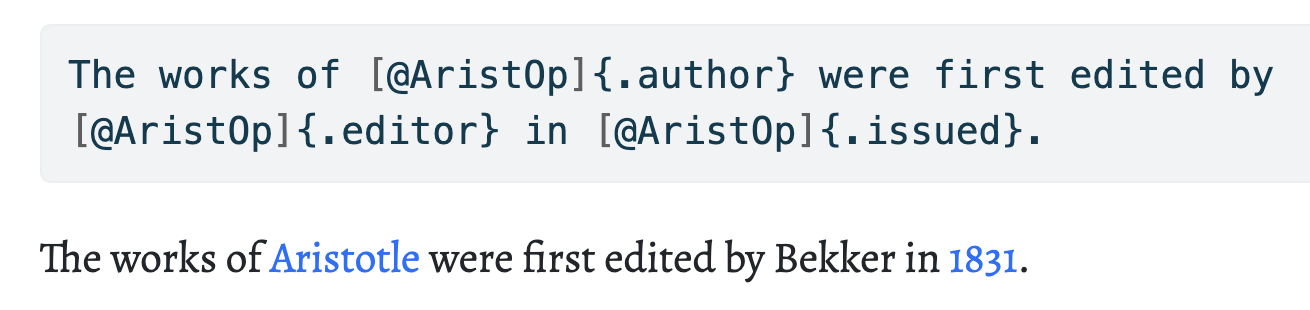
\includegraphics[width=4.63542in,height=4.77083in]{citefield.png}

}

\caption{\label{fig-scriv44}Printed page with many examples of the
citation markup employed by Cite Tools.}

\end{figure}

\textsc{For the Cite Field filter,} \textbf{Character Styles} provide
support for the Cite Field Lua Filter, which can be used to cite
arbitrary fields of the references.

\begin{quote}
The works of \texttt{{[}@AristOp{]}\{.author\}} were first edited by
\texttt{{[}@AristOp{]}\{.editor\}} in
\texttt{{[}@AristOp{]}\{.issued\}}.\\
The works of Aristotelis were first edited by Bekker in 1834.
\end{quote}

\begin{quote}
Later, the \texttt{{[}@DA{]}\{.title\}}
(\texttt{{[}@DA{]}\{.title-short\}}) was edited by
\texttt{{[}@DABiehl1896{]}\{.editor\}} in
\texttt{{[}@DABiehl1896{]}\{.issued\}} (reprinted in
\texttt{{[}@DATheiler{]}\{.translator\}\textquotesingle{}s}
\texttt{{[}@DATheiler{]}\{.issued\}} translation).\\
Later, the \emph{De Anima} was edited by Biehl in 1896 (reprinted in
{\protect\hypertarget{cite_93}{}{\label{cite_93}Aristotelis
(\protect\hyperlink{ref-DATheiler}{1995})}}'s 1995 translation).
\end{quote}

\begin{tcolorbox}[enhanced jigsaw, left=2mm, colframe=quarto-callout-warning-color-frame, bottomtitle=1mm, colback=white, coltitle=black, title=\textcolor{quarto-callout-warning-color}{\faExclamationTriangle}\hspace{0.5em}{Warning}, toprule=.15mm, rightrule=.15mm, opacityback=0, breakable, toptitle=1mm, titlerule=0mm, colbacktitle=quarto-callout-warning-color!10!white, arc=.35mm, bottomrule=.15mm, leftrule=.75mm, opacitybacktitle=0.6]

You can set link-fields to false to avoid undesired linking when citing
specific fields.

\end{tcolorbox}

Here is a printout of different citation fields followed by a concrete
example of how to use them in a document.

\begin{longtable}[]{@{}
  >{\centering\arraybackslash}p{(\columnwidth - 2\tabcolsep) * \real{0.5000}}
  >{\centering\arraybackslash}p{(\columnwidth - 2\tabcolsep) * \real{0.5000}}@{}}
\toprule\noalign{}
\begin{minipage}[b]{\linewidth}\centering
Raw
\end{minipage} & \begin{minipage}[b]{\linewidth}\centering
Output
\end{minipage} \\
\midrule\noalign{}
\endfirsthead
\toprule\noalign{}
\begin{minipage}[b]{\linewidth}\centering
Raw
\end{minipage} & \begin{minipage}[b]{\linewidth}\centering
Output
\end{minipage} \\
\midrule\noalign{}
\endhead
\bottomrule\noalign{}
\endlastfoot
Aristotelis & Aristotelis \\
Bekker & Bekker \\
\emph{Aristotelis Opera} & \emph{Aristotelis Opera} \\
1834 & 1834\footnote{Note that
  \protect\hypertarget{cite_94}{}{\label{cite_94}(\protect\hyperlink{ref-AristOp}{1834a})}
  would render as
  \protect\hypertarget{cite_95}{}{\label{cite_95}(\protect\hyperlink{ref-AristOp}{1834a})}.} \\
Reimer & Reimer \\
Berlin & Berlin \\
{\protect\hypertarget{cite_96}{}{\label{cite_96}Aristotelis
(\protect\hyperlink{ref-AristOp}{1834a})}} &
{\protect\hypertarget{cite_97}{}{\label{cite_97}Aristotelis
(\protect\hyperlink{ref-AristOp}{1834a})}} \\
{\protect\hypertarget{cite_98}{}{\label{cite_98}Aristotelis
(\protect\hyperlink{ref-AristOp}{1834a})}} &
{\protect\hypertarget{cite_99}{}{\label{cite_99}Aristotelis
(\protect\hyperlink{ref-AristOp}{1834a})}} \\
\caption{Printout of different fields from the reference}\tabularnewline
\end{longtable}

The first critical edition of Aristotle's works was published by Bekker
in 1834.
\texttt{The\ first\ critical\ edition\ of\ Aristotle\textquotesingle{}s\ works\ was\ published\ by\ {[}@AristOp{]}\{.editor\}\ in\ {[}@AristOp{]}\{.issued\}.}
:::

\hypertarget{tbl-scriv46}{}
\begin{longtable}[]{@{}
  >{\centering\arraybackslash}p{(\columnwidth - 4\tabcolsep) * \real{0.3333}}
  >{\centering\arraybackslash}p{(\columnwidth - 4\tabcolsep) * \real{0.3333}}
  >{\centering\arraybackslash}p{(\columnwidth - 4\tabcolsep) * \real{0.3333}}@{}}
\toprule\noalign{}
\begin{minipage}[b]{\linewidth}\centering
\href{https://docs.citationstyles.org/en/stable/specification.html\#appendix-iii-types}{CSL}
\end{minipage} & \begin{minipage}[b]{\linewidth}\centering
\href{https://en.wikipedia.org/wiki/BibTeX\#Entry_types}{BibTeX}
\end{minipage} & \begin{minipage}[b]{\linewidth}\centering
\href{https://en.wikipedia.org/wiki/RIS_(file_format)\#Type_of_reference}{RIS}
\end{minipage} \\
\midrule\noalign{}
\endfirsthead
\toprule\noalign{}
\begin{minipage}[b]{\linewidth}\centering
\href{https://docs.citationstyles.org/en/stable/specification.html\#appendix-iii-types}{CSL}
\end{minipage} & \begin{minipage}[b]{\linewidth}\centering
\href{https://en.wikipedia.org/wiki/BibTeX\#Entry_types}{BibTeX}
\end{minipage} & \begin{minipage}[b]{\linewidth}\centering
\href{https://en.wikipedia.org/wiki/RIS_(file_format)\#Type_of_reference}{RIS}
\end{minipage} \\
\midrule\noalign{}
\endhead
\bottomrule\noalign{}
\endlastfoot
article-journal & article & JOUR JFULL INPR \\
book & book proceedings manual & ANCIENT BOOK CLSWK DICT EBOOK EDBOOK \\
pamphlet & booklet & PAMP \\
chapter & inbook incollection & CHAP ECHAP \\
paper-conference & inproceedings & CONF CPAPER \\
thesis & mastersthesis phdthesis misc & THES \\
report & techreport & GOVDOC GRANT HEAR RPRT STAND \\
manuscript & unpublished & MANSCPT \\
\caption{\label{tbl-scriv46}CSL-YAML/CSL-JSON types alongside their
BibTeX and RIS equivalents. Notice how we are using HTML line breaks to
create lists inside table cells.}\tabularnewline
\end{longtable}

\hypertarget{tbl-scriv47}{}
\begin{longtable}[]{@{}
  >{\centering\arraybackslash}p{(\columnwidth - 4\tabcolsep) * \real{0.3333}}
  >{\centering\arraybackslash}p{(\columnwidth - 4\tabcolsep) * \real{0.3333}}
  >{\centering\arraybackslash}p{(\columnwidth - 4\tabcolsep) * \real{0.3333}}@{}}
\toprule\noalign{}
\begin{minipage}[b]{\linewidth}\centering
\href{https://docs.citationstyles.org/en/stable/specification.html\#appendix-iv-variables}{CSL
variables}
\end{minipage} & \begin{minipage}[b]{\linewidth}\centering
\href{https://en.wikipedia.org/wiki/BibTeX\#Field_types}{BibTeX Fields}
\end{minipage} & \begin{minipage}[b]{\linewidth}\centering
\href{https://en.wikipedia.org/wiki/RIS_(file_format)\#Tags}{RIS Tags}
\end{minipage} \\
\midrule\noalign{}
\endfirsthead
\toprule\noalign{}
\begin{minipage}[b]{\linewidth}\centering
\href{https://docs.citationstyles.org/en/stable/specification.html\#appendix-iv-variables}{CSL
variables}
\end{minipage} & \begin{minipage}[b]{\linewidth}\centering
\href{https://en.wikipedia.org/wiki/BibTeX\#Field_types}{BibTeX Fields}
\end{minipage} & \begin{minipage}[b]{\linewidth}\centering
\href{https://en.wikipedia.org/wiki/RIS_(file_format)\#Tags}{RIS Tags}
\end{minipage} \\
\midrule\noalign{}
\endhead
\bottomrule\noalign{}
\endlastfoot
abstract & abstract & AB \\
author & authors & AU A1 \\
call-number & library & ID \\
chapter-number collection-number number issue & chapter number issue &
IS \\
collection-title & series & - \\
container-title & booktitle journal & BT T2 JA JF JO \\
DOI & doi & DO \\
editor & editors & A2 ED \\
genre & type & - \\
ISSN & issn & SN \\
issued & date & PY Y1 \\
keywords & keywords & KW \\
language & langid & LA \\
number-of-volumes & volumes & NV \\
original-title & origtitle & OR* \\
page & pages & SP EP \\
publisher & publisher school institution organization howpublished &
PB \\
publisher-place & address & PP \\
title & title & TI T1 CT \\
title-short & shorttitle & ST* \\
url & URL & UR LK \\
version & version & - \\
volume & volume & VL \\
\caption{\label{tbl-scriv47}CSL-YAML/CSL-JSON variables alongside
corresponding
\href{https://github.com/jgm/pandoc/blob/main/src/Text/Pandoc/Citeproc/BibTeX.hs}{BibTeX}
fields and
\href{https://github.com/jgm/pandoc/blob/main/src/Text/Pandoc/Readers/RIS.hs}{RIS}
tags. Those marked with an asterisk exist and correspond, but, for some
reason, Pandoc ignores them instead of converting to
CSL.}\tabularnewline
\end{longtable}

\hypertarget{tbl-scriv48}{}
\begin{longtable}[]{@{}ccc@{}}
\toprule\noalign{}
CSL Field & Markdown Source & Output \\
\midrule\noalign{}
\endfirsthead
\toprule\noalign{}
CSL Field & Markdown Source & Output \\
\midrule\noalign{}
\endhead
\bottomrule\noalign{}
\endlastfoot
Author & \texttt{{[}@AristOp{]}\{.author\}} & Aristotelis \\
Editor & \texttt{{[}@AristOp{]}\{.editor\}} & Bekker \\
Issued & \texttt{{[}@AristOp{]}\{.issued\}} & 1834 \\
Original-title & \texttt{{[}@DA{]}\{.original-title\}} &
{\protect\hypertarget{cite_100}{}{\label{cite_100}Aristotelis
(\protect\hyperlink{ref-DA}{1834b})}} \\
Publisher & \texttt{{[}@AristOp{]}\{.publisher\}} & Reimer \\
Publisher-place & \texttt{AristOp} & AristOp \\
Title & \texttt{{[}@AristOp{]}\{.title\}} & \emph{Aristotelis Opera} \\
Title-short & \texttt{{[}@AristOp{]}\{.title-short\}} &
{\protect\hypertarget{cite_101}{}{\label{cite_101}Aristotelis
(\protect\hyperlink{ref-AristOp}{1834a})}} \\
Translator & \texttt{{[}@DABiehl1896\ {]}\{.editor\}} & Biehl \\
Translator & \texttt{{[}@DATheiler{]}\{.translator\}} &
{\protect\hypertarget{cite_102}{}{\label{cite_102}Aristotelis
(\protect\hyperlink{ref-DATheiler}{1995})}} \\
\caption{\label{tbl-scriv48}Simple example of how we are using styles to
create the correct markup}\tabularnewline
\end{longtable}

\hypertarget{sec-scriv49}{%
\section{Multipart Bibliography}\label{sec-scriv49}}

\protect\hypertarget{scriv49}{}{}

In many areas of research, the ability to split the bibliography into
sections is a condition \emph{sine qua non} for publishing. In the
humanities, for example, there are usually \emph{primary} and
\emph{secondary} sources. In philosophy, even, they can be very nuanced
with sections dedicated to original sources, translations, commentaries,
and so on. The \textbf{Section Type} titled
\texttt{Multipart\ Bibliography} can be used to create as many new
bibliography sections as necessary. Add to the text the references that
should print there, and let it know in the custom metadata
\texttt{\textless{}\textbackslash{}\$custom:Attributes\textgreater{}}
the format being used (\emph{e.g.} \texttt{bib}, \texttt{yml},
\texttt{ris}).

\begin{tcolorbox}[enhanced jigsaw, left=2mm, colframe=quarto-callout-tip-color-frame, bottomtitle=1mm, colback=white, coltitle=black, title=\textcolor{quarto-callout-tip-color}{\faLightbulb}\hspace{0.5em}{Bibliography formats}, toprule=.15mm, rightrule=.15mm, opacityback=0, breakable, toptitle=1mm, titlerule=0mm, colbacktitle=quarto-callout-tip-color!10!white, arc=.35mm, bottomrule=.15mm, leftrule=.75mm, opacitybacktitle=0.6]

Speaking about formats, the most common bibliography formats are
\href{https://docs.citationstyles.org/en/stable/specification.html}{CSL-YAML},
\href{https://docs.citationstyles.org/en/stable/specification.html}{CSL-JSON},
\href{https://en.wikipedia.org/wiki/BibTeX\#Entry_types}{BibTeX}, and
\href{https://en.wikipedia.org/wiki/RIS_(file_format)\#Type_of_reference}{RIS}.
Internally, \textbf{Pandoc} and \textbf{Quarto} use the CSL
(\textbf{C}itation \textbf{S}tyle \textbf{L}anguage) to handle
bibliography, so \textbf{CSL-YAML} and \textbf{CSL-JSON} perform much
better (up to 10 times faster) than older formats like \textbf{BibTeX}
or \textbf{RIS} that will have to be converted by \textbf{Pandoc} before
it can be understood.

\end{tcolorbox}

ScrivQ provides all the data needed for the project to compile. Before
you can use Citeproc on your projects, you will need to generate your
bibliography data. In principle, nothing stops you from manually, or
semi-manually, keeping a bibliography in Scrivener, but this is not very
easy to manage if you have many projects sharing the same references.
(Luckily, in this regard, Scrivener offers the best text comparison
tools I can think of). The best alternative, it seems, is to rely on
specialized software such as Zotero, Bookends, Bibdesk (also JabRef,
Endnote, and
\href{en.wikipedia.org/wiki/Comparison_of_reference_management_software}{others}).
These programs allow you to edit your bibliography and easily export it
in the desired format, which can be copied and pasted to different
Scrivener projects. Zotero even offers an API that can be used to
download shared libraries by merely accessing a link, such as
\texttt{https://api.zotero.org/groups/}\ul{LibraryID}\texttt{/items?format=bibtex\&limit=999}
where \texttt{LibraryID} corresponds to the library's 7-digit code
(visible in the middle of the library URL).

\begin{figure}

{\centering 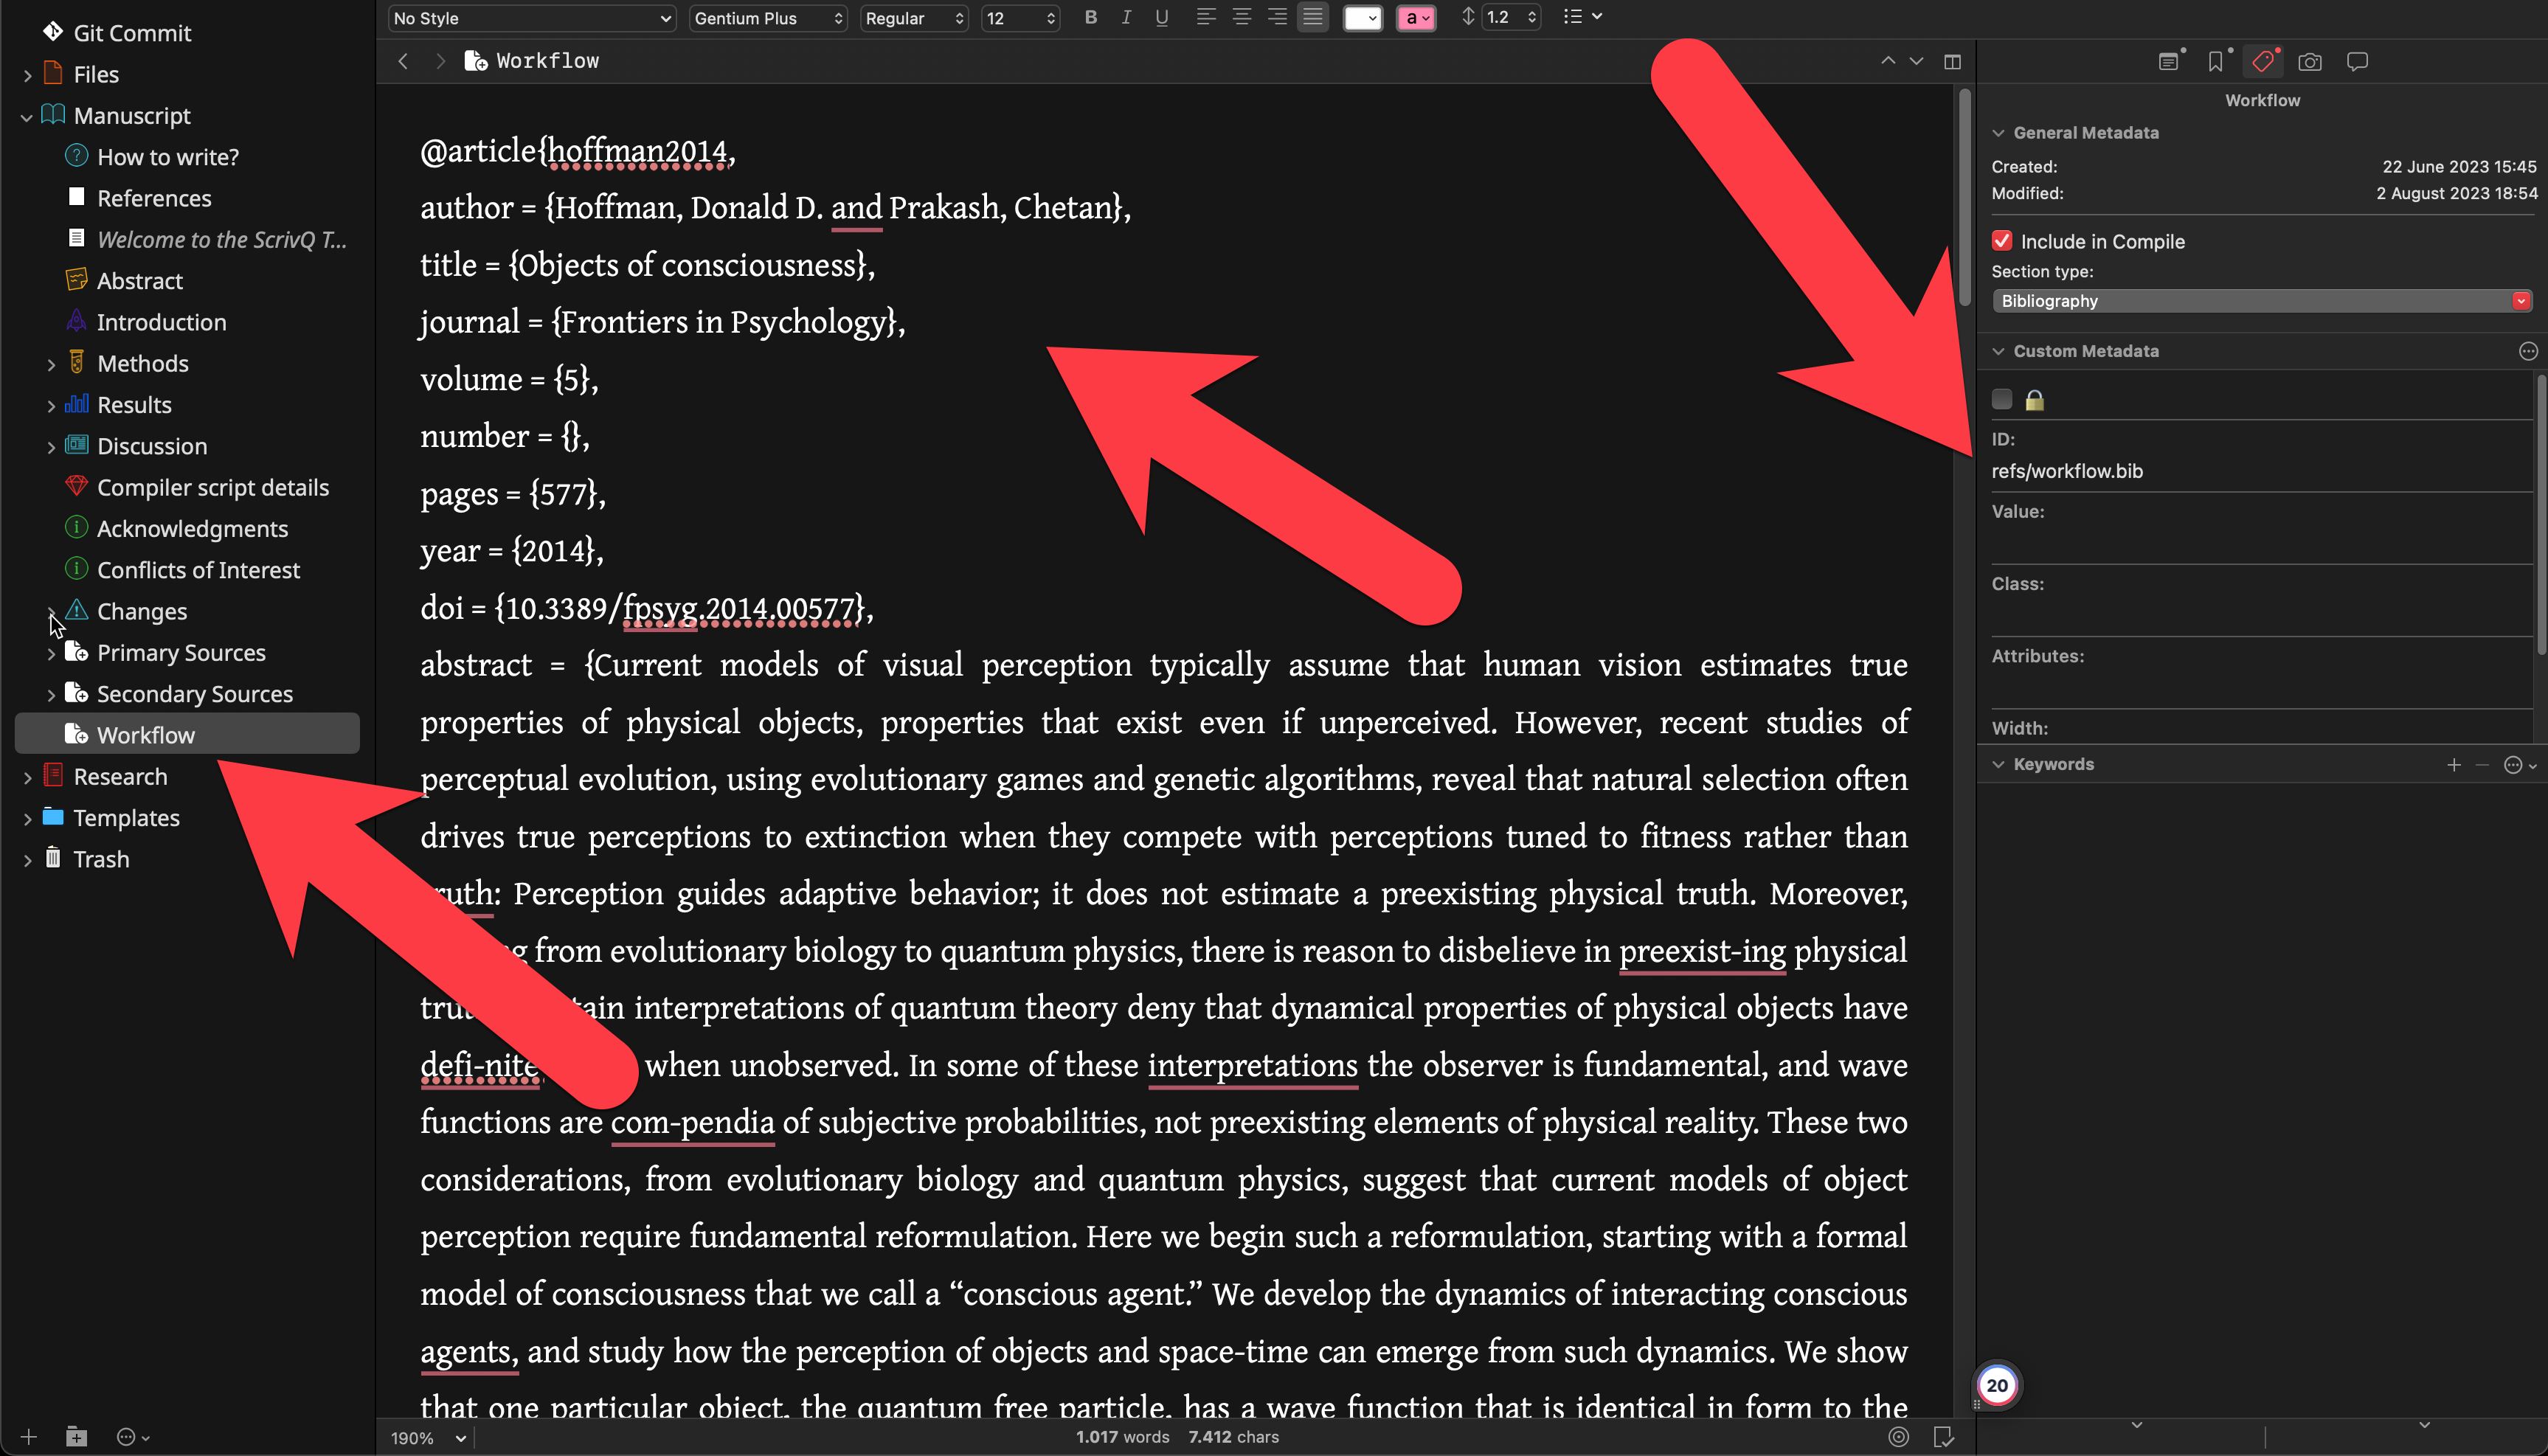
\includegraphics[width=4.02083in,height=2.30208in]{newbibliography.png}

}

\caption{\label{fig-scriv49A}This will result in a separate file, whose
path will be added to the front matter, with the content of the text.
The resulting bibliography will print right where we placed it in our
project.}

\end{figure}

\begin{figure}

{\centering 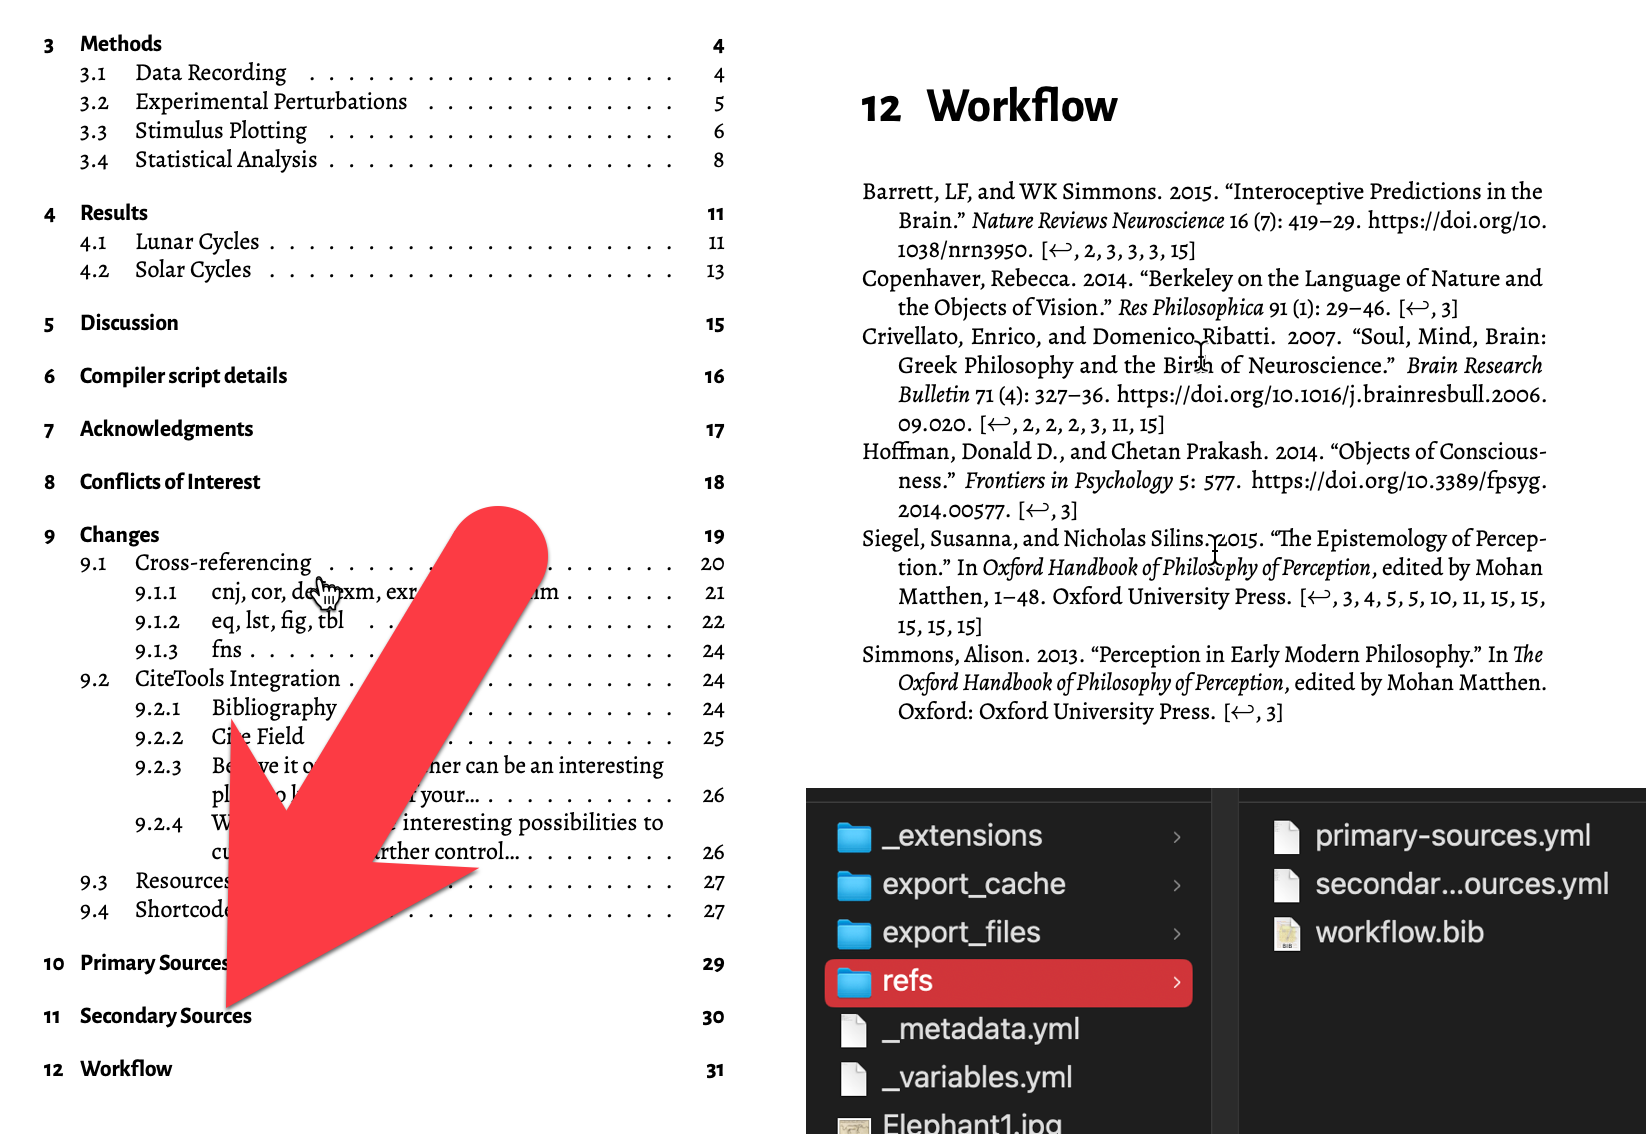
\includegraphics[width=4.45833in,height=3.07292in]{resultbib.png}

}

\caption{\label{fig-scriv49B}On the left we have the \textbf{Table of
Contents}; on the top-right, we see the printed bibliography (page 31)
and, on the bottom-right, the files are automatically created during the
compilation process.}

\end{figure}

\begin{tcolorbox}[enhanced jigsaw, left=2mm, colframe=quarto-callout-important-color-frame, bottomtitle=1mm, colback=white, coltitle=black, title=\textcolor{quarto-callout-important-color}{\faExclamation}\hspace{0.5em}{The sky is the limit}, toprule=.15mm, rightrule=.15mm, opacityback=0, breakable, toptitle=1mm, titlerule=0mm, colbacktitle=quarto-callout-important-color!10!white, arc=.35mm, bottomrule=.15mm, leftrule=.75mm, opacitybacktitle=0.6]

You can add as many bibliographies as you want!

\end{tcolorbox}

\begin{tcolorbox}[enhanced jigsaw, left=2mm, colframe=quarto-callout-tip-color-frame, bottomtitle=1mm, colback=white, coltitle=black, title=\textcolor{quarto-callout-tip-color}{\faLightbulb}\hspace{0.5em}{Bibliography files in the system}, toprule=.15mm, rightrule=.15mm, opacityback=0, breakable, toptitle=1mm, titlerule=0mm, colbacktitle=quarto-callout-tip-color!10!white, arc=.35mm, bottomrule=.15mm, leftrule=.75mm, opacitybacktitle=0.6]

As you can see, there is no need to keep separate bibliography files in
the system. You can simply copy and paste the data from your
bibliography manager to Scrivener. If you are using macOS, check
Bookends and Bibdesk; and, on all platforms, definitively get Zotero as
well.

\end{tcolorbox}

\begin{tcolorbox}[enhanced jigsaw, left=2mm, colframe=quarto-callout-note-color-frame, bottomtitle=1mm, colback=white, coltitle=black, title=\textcolor{quarto-callout-note-color}{\faInfo}\hspace{0.5em}{From structured bibliography data to the rendered output}, toprule=.15mm, rightrule=.15mm, opacityback=0, breakable, toptitle=1mm, titlerule=0mm, colbacktitle=quarto-callout-note-color!10!white, arc=.35mm, bottomrule=.15mm, leftrule=.75mm, opacitybacktitle=0.6]

We are feeding the data precisely where you would usually write out your
references. In this case, however, we provide the structured data and
let Citeproc determine how to display it based on the CSL file rules.

\end{tcolorbox}

\hypertarget{sec-scriv50}{%
\section{Citation Style Language}\label{sec-scriv50}}

\protect\hypertarget{scriv50}{}{}

\begin{tcolorbox}[enhanced jigsaw, left=2mm, colframe=quarto-callout-note-color-frame, bottomtitle=1mm, colback=white, coltitle=black, title=\textcolor{quarto-callout-note-color}{\faInfo}\hspace{0.5em}{Note}, toprule=.15mm, rightrule=.15mm, opacityback=0, breakable, toptitle=1mm, titlerule=0mm, colbacktitle=quarto-callout-note-color!10!white, arc=.35mm, bottomrule=.15mm, leftrule=.75mm, opacitybacktitle=0.6]

Did you notice that we used \texttt{{[}@AristOp{]}\{.issued\}} instead
of \st{\mbox{\texttt{{[}@AristOp{]}\{.date\}}}}? And \texttt{AristOp}
instead of \st{\mbox{\texttt{{[}@AristOp{]}\{.city\}}}}?

\end{tcolorbox}

{[}{]}{[}226091195-7b27f8a7-c802-4cbb-bac9-81265b7aed45{]}

\hypertarget{sec-scriv51}{%
\section{Citation Backlinks}\label{sec-scriv51}}

\protect\hypertarget{scriv51}{}{}

In the vanilla Pandoc Citeproc, you can use link-citations to control
whether citations in the body of the text should be clickable links to
the reference in the bibliography
(e.g.~{\protect\hypertarget{cite_103}{}{\label{cite_103}(\protect\hyperlink{ref-EN}{\textbf{EN?}})}}).
This is a very useful feature, especially when you want to quickly check
the source of a citation without having to scroll through the whole
text.

::: \{.callout-tip appearance=\enquote{simple}\} The citetools extension
will take this one step further and add, in a crescent ordinal fashion
{[}1, 2, 3, 4{]}\footnote{In other output formats, such as PDF, the
  reader will see the page number instead of a crescent ordinal number.},
a backlink to each citation an entry has received in the document. :::
This allows the reader to easily arrive at sections of the text where
the same reference was discussed, quickly seeing with the array of
backlinks, how many times each reference was used in the text (see
reference at the bottom of the text).

\hypertarget{sec-scriv52}{%
\subsection{How to avoid an excess of undesired
links}\label{sec-scriv52}}

\protect\hypertarget{scriv52}{}{}

In citetools there are options to avoid undesired linking and anomalies
caused by citing individual fields, such as repeated links to the same
entry in a single phrase or section.

First, there is the option to force a citation to not be a link by
adding a simple dot at the end of the .csl\_field.

\begin{longtable}[]{@{}ll@{}}
\toprule\noalign{}
Default & Link--suppresion \\
\midrule\noalign{}
\endhead
\bottomrule\noalign{}
\endlastfoot
{\protect\hypertarget{cite_104}{}{\label{cite_104}(\protect\hyperlink{ref-EN}{\textbf{EN?}})}}
&
{\protect\hypertarget{cite_105}{}{\label{cite_105}(\protect\hyperlink{ref-EN}{\textbf{EN?}})}} \\
{\protect\hypertarget{cite_106}{}{\label{cite_106}(\protect\hyperlink{ref-EN}{\textbf{EN?}})}}
&
{\protect\hypertarget{cite_107}{}{\label{cite_107}(\protect\hyperlink{ref-EN}{\textbf{EN?}})}} \\
\end{longtable}

Then, there is also the global link-fields option, which allows the user
to turn off links in citations that target individual fields. It can be
used in conjunction with other options that target the bibliography,
such as link-citations and link-bibliography. link-citations: true \#
\textless1\textgreater{} link-fields: true \# \textless2\textgreater{}
link-bibliography: true \# \textless3\textgreater{} lang: en-ZA \#
\textless4\textgreater{}

\begin{enumerate}
\def\labelenumi{\arabic{enumi}.}
\tightlist
\item
  Hyperlink citations to the corresponding bibliography entries.
  Defaults to false.
\item
  Hyperlink citations that target specific CSL fields to the
  corresponding entries in the bibliography. If link-citations is true,
  this defaults to true.
\item
  Hyperlink DOIs, PMCIDs, PMID, and URLs in bibliographies. Defaults to
  true.
\item
  Affects the bibliography tags. Defaults to en-US.
\end{enumerate}

\hypertarget{sec-scriv53}{%
\section{About}\label{sec-scriv53}}

\protect\hypertarget{scriv53}{}{}

Logo image generated Dall-E using Enso-like round black and white
painting with ancient greek war-ship with man tied to the mast as
prompt. License Filters published under the MIT license by Albert
Krewinkel (tarleb).

\begin{itemize}
\tightlist
\item
  multibib
\item
  multiple-bibliographies
\item
  citation-backlinks
\item
  section-bibliographies
\end{itemize}

Filters published under the MIT license by Albert Krewinkel (tarleb) \&
Bernardo Vasconcelos (bcdavasconcelos).

\begin{itemize}
\tightlist
\item
  citefield
\end{itemize}

All Pandoc Lua filters in this extension are published under the MIT
license, see file LICENSE for details. The Cite Tools Documentation is
under a Creative Commons Attribution-NonCommercial 4.0 International
License.

\begin{figure}

{\centering 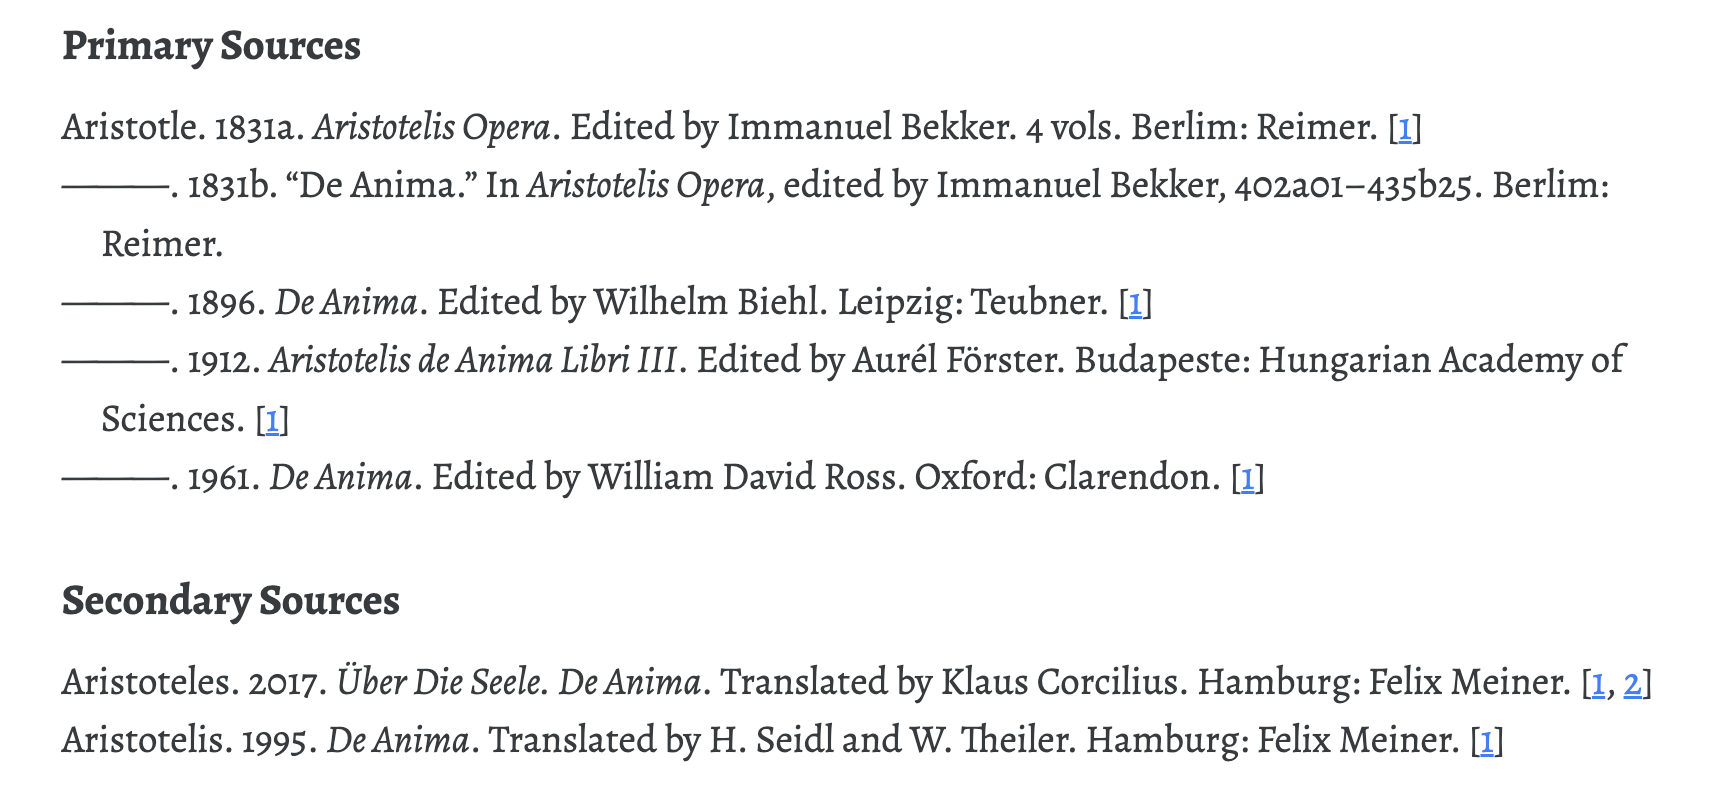
\includegraphics[width=4.70833in,height=2.15625in]{multipartbibliography.png}

}

\caption{\label{fig-scriv54A}Multipart bibliography with sections, such
as primary sources and secondary sources}

\end{figure}

\begin{figure}

{\centering 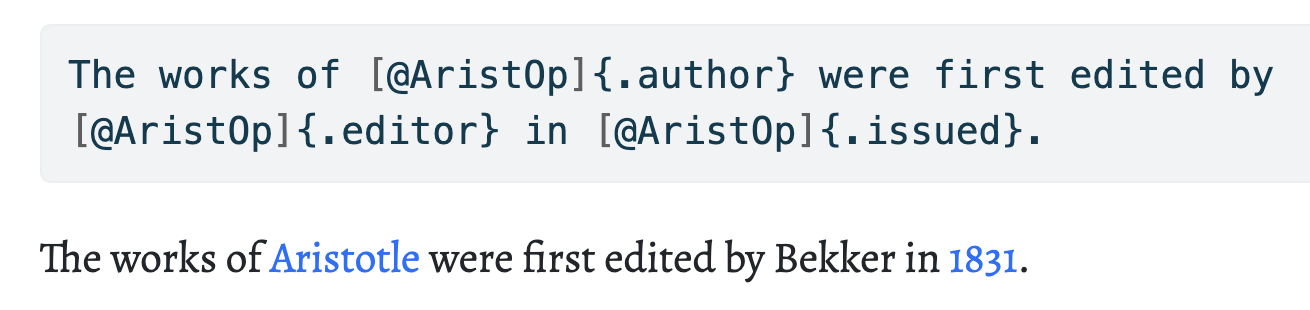
\includegraphics[width=4.75in,height=1.125in]{citefield.png}

}

\caption{\label{fig-scriv54B}Cite Field allows the evocation of
arbitrary information from the references, such as \texttt{author},
\texttt{editor}, \texttt{translator} (using
\href{https://docs.citationstyles.org/en/stable/specification.html\#appendix-iv-variables}{CSL
variables} name conventions)}

\end{figure}

\begin{figure}

{\centering 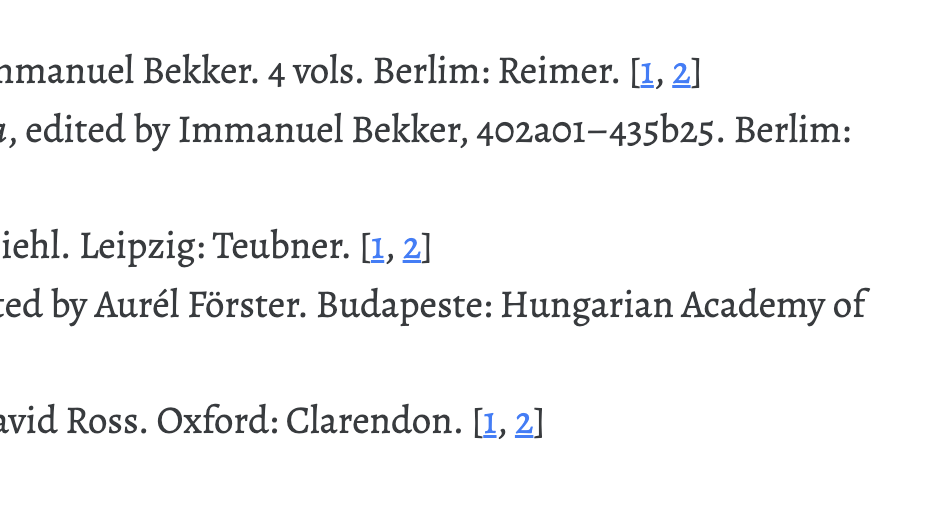
\includegraphics[width=4.84375in,height=2.6875in]{backrefs.png}

}

\caption{\label{fig-scriv54C}The \textbf{Citation Backlinks} filter adds
an index of cited references to the bibliography, with links back to all
in-text citations. It also allows the user to turn these off globally or
in an \emph{ad hoc} fashion.}

\end{figure}

\hypertarget{scriv55}{}
\begin{figure*}

\leavevmode\vadjust pre{\hypertarget{first-column}{}}%
\textbf{BibTeX}

\begin{Shaded}
\begin{Highlighting}[numbers=left,,]
\VariableTok{@book}\NormalTok{\{}\OtherTok{AristOp}\NormalTok{,}
\DataTypeTok{author}\NormalTok{ = \{Aristotle\},}
\DataTypeTok{editor}\NormalTok{ = \{Bekker, Immanuel\},}
\DataTypeTok{title}\NormalTok{ = \{Aristotelis opera\},}
\DataTypeTok{publisher}\NormalTok{ = \{Reimer\},}
\DataTypeTok{address}\NormalTok{ = \{Berlim\},}
\DataTypeTok{volumes}\NormalTok{ = \{4\},}
\DataTypeTok{edition}\NormalTok{ = \{1\},}
\DataTypeTok{year}\NormalTok{ = \{1831\}}
\NormalTok{\}}
\end{Highlighting}
\end{Shaded}

\textbf{RIS}

\begin{Shaded}
\begin{Highlighting}[numbers=left,,]
\NormalTok{TY  {-} BOOK}
\NormalTok{ID  {-} AristOp}
\NormalTok{AU  {-} Aristotle}
\NormalTok{ED  {-} Bekker, Immanuel}
\NormalTok{TI  {-} Aristotelis opera}
\NormalTok{PB  {-} Reimer}
\NormalTok{CY  {-} Berlim}
\NormalTok{ET  {-} 1}
\NormalTok{VL  {-} 4}
\NormalTok{Y1  {-} 1831}
\NormalTok{ER  {-}}
\end{Highlighting}
\end{Shaded}

\hypertarget{second-column}{}

\leavevmode\vadjust pre{\hypertarget{forth-column}{}}%
\textbf{CSL-YAML}

\begin{Shaded}
\begin{Highlighting}[numbers=left,,]
\PreprocessorTok{{-}{-}{-}}
\FunctionTok{references}\KeywordTok{:}
\KeywordTok{{-}}\AttributeTok{ }\FunctionTok{author}\KeywordTok{:}
\AttributeTok{  }\KeywordTok{{-}}\AttributeTok{ }\FunctionTok{family}\KeywordTok{:}\AttributeTok{ Aristotle}
\AttributeTok{  }\FunctionTok{edition}\KeywordTok{:}\AttributeTok{ }\DecValTok{1}
\AttributeTok{  }\FunctionTok{editor}\KeywordTok{:}
\AttributeTok{  }\KeywordTok{{-}}\AttributeTok{ }\FunctionTok{family}\KeywordTok{:}\AttributeTok{ Bekker}
\AttributeTok{    }\FunctionTok{given}\KeywordTok{:}\AttributeTok{ Immanuel}
\AttributeTok{  }\FunctionTok{id}\KeywordTok{:}\AttributeTok{ AristOp}
\AttributeTok{  }\FunctionTok{issued}\KeywordTok{:}\AttributeTok{ }\DecValTok{1831}
\AttributeTok{  }\FunctionTok{number{-}of{-}volumes}\KeywordTok{:}\AttributeTok{ }\DecValTok{4}
\AttributeTok{  }\FunctionTok{publisher}\KeywordTok{:}\AttributeTok{ Reimer}
\AttributeTok{  }\FunctionTok{publisher{-}place}\KeywordTok{:}\AttributeTok{ Berlim}
\AttributeTok{  }\FunctionTok{title}\KeywordTok{:}\AttributeTok{ Aristotelis opera}
\AttributeTok{  }\FunctionTok{type}\KeywordTok{:}\AttributeTok{ book}
\PreprocessorTok{{-}{-}{-}}
\end{Highlighting}
\end{Shaded}

\textbf{CSL-JSON}

\begin{Shaded}
\begin{Highlighting}[numbers=left,,]
\OtherTok{[}
  \FunctionTok{\{}
    \DataTypeTok{"author"}\FunctionTok{:} \OtherTok{[}
      \FunctionTok{\{}
        \DataTypeTok{"family"}\FunctionTok{:} \StringTok{"Aristotle"}
      \FunctionTok{\}}
    \OtherTok{]}\FunctionTok{,}
    \DataTypeTok{"edition"}\FunctionTok{:} \StringTok{"1"}\FunctionTok{,}
    \DataTypeTok{"editor"}\FunctionTok{:} \OtherTok{[}
      \FunctionTok{\{}
        \DataTypeTok{"family"}\FunctionTok{:} \StringTok{"Bekker"}\FunctionTok{,}
        \DataTypeTok{"given"}\FunctionTok{:} \StringTok{"Immanuel"}
      \FunctionTok{\}}
    \OtherTok{]}\FunctionTok{,}
    \DataTypeTok{"id"}\FunctionTok{:} \StringTok{"AristOp"}\FunctionTok{,}
    \DataTypeTok{"issued"}\FunctionTok{:} \FunctionTok{\{}
      \DataTypeTok{"date{-}parts"}\FunctionTok{:} \OtherTok{[}
        \OtherTok{[}
          \DecValTok{1831}
        \OtherTok{]}
      \OtherTok{]}
    \FunctionTok{\},}
    \DataTypeTok{"number{-}of{-}volumes"}\FunctionTok{:} \StringTok{"4"}\FunctionTok{,}
    \DataTypeTok{"publisher"}\FunctionTok{:} \StringTok{"Reimer"}\FunctionTok{,}
    \DataTypeTok{"publisher{-}place"}\FunctionTok{:} \StringTok{"Berlim"}\FunctionTok{,}
    \DataTypeTok{"title"}\FunctionTok{:} \StringTok{"Aristotelis opera"}\FunctionTok{,}
    \DataTypeTok{"type"}\FunctionTok{:} \StringTok{"book"}
  \FunctionTok{\}}
\OtherTok{]}
\end{Highlighting}
\end{Shaded}

\end{figure*}

\hypertarget{sec-scriv56}{%
\chapter{Primary Sources}\label{sec-scriv56}}

\hypertarget{refs_scriv56}{}
\begin{CSLReferences}{1}{0}
\leavevmode\vadjust pre{\hypertarget{ref-AristOp}{}}%
Aristotelis. 1834a. \emph{Aristotelis Opera}. Edited by I. Bekker.
Berlin: Reimer. {[}\Acrobatmenu{GoBack}{$\hookleftarrow$},
\protect\hyperlink{cite_94}{\pageref{cite_94}},
\protect\hyperlink{cite_95}{\pageref{cite_95}},
\protect\hyperlink{cite_96}{\pageref{cite_96}},
\protect\hyperlink{cite_97}{\pageref{cite_97}},
\protect\hyperlink{cite_98}{\pageref{cite_98}},
\protect\hyperlink{cite_99}{\pageref{cite_99}},
\protect\hyperlink{cite_101}{\pageref{cite_101}}{]}

\leavevmode\vadjust pre{\hypertarget{ref-DA}{}}%
---------. 1834b. {``De Anima.''} In \emph{Aristotelis Opera}, edited by
I. Bekker. Berlin: Reimer. {[}\Acrobatmenu{GoBack}{$\hookleftarrow$},
\protect\hyperlink{cite_100}{\pageref{cite_100}}{]}

\end{CSLReferences}

\hypertarget{sec-scriv83}{%
\chapter{Secondary Sources}\label{sec-scriv83}}

\hypertarget{refs_scriv83}{}
\begin{CSLReferences}{1}{0}
\leavevmode\vadjust pre{\hypertarget{ref-DABiehl1896}{}}%
Aristotelis. 1896. \emph{De Anima}. Edited by Wilhelm Biehl. Leipzig:
Teubner. {[}\Acrobatmenu{GoBack}{$\hookleftarrow$}{]}

\leavevmode\vadjust pre{\hypertarget{ref-DATheiler}{}}%
---------. 1995. \emph{De Anima}. Edited by Willy Theiler and Horst
Seidl. Harmburg: Felix Meiner.
{[}\Acrobatmenu{GoBack}{$\hookleftarrow$},
\protect\hyperlink{cite_93}{\pageref{cite_93}},
\protect\hyperlink{cite_102}{\pageref{cite_102}}{]}

\leavevmode\vadjust pre{\hypertarget{ref-Long2004}{}}%
Long, Christopher. 2004. \emph{Ethics of Ontology}. SUNY Series in
Ancient Greek Philosophy. Albany: SUNY.
{[}\Acrobatmenu{GoBack}{$\hookleftarrow$},
\protect\hyperlink{cite_80}{\pageref{cite_80}},
\protect\hyperlink{cite_81}{\pageref{cite_81}},
\protect\hyperlink{cite_82}{\pageref{cite_82}},
\protect\hyperlink{cite_83}{\pageref{cite_83}},
\protect\hyperlink{cite_84}{\pageref{cite_84}},
\protect\hyperlink{cite_85}{\pageref{cite_85}},
\protect\hyperlink{cite_86}{\pageref{cite_86}},
\protect\hyperlink{cite_87}{\pageref{cite_87}},
\protect\hyperlink{cite_88}{\pageref{cite_88}},
\protect\hyperlink{cite_89}{\pageref{cite_89}},
\protect\hyperlink{cite_90}{\pageref{cite_90}},
\protect\hyperlink{cite_91}{\pageref{cite_91}}{]}

\end{CSLReferences}

\hypertarget{sec-scriv129}{%
\chapter{Workflow}\label{sec-scriv129}}

\hypertarget{refs_scriv129}{}
\begin{CSLReferences}{1}{0}
\leavevmode\vadjust pre{\hypertarget{ref-barrett2015}{}}%
Barrett, LF, and WK Simmons. 2015. {``Interoceptive Predictions in the
Brain.''} \emph{Nature Reviews Neuroscience} 16 (7): 419--29.
\url{https://doi.org/10.1038/nrn3950}.
{[}\Acrobatmenu{GoBack}{$\hookleftarrow$},
\protect\hyperlink{cite_109}{\pageref{cite_109}},
\protect\hyperlink{cite_114}{\pageref{cite_114}},
\protect\hyperlink{cite_115}{\pageref{cite_115}},
\protect\hyperlink{cite_116}{\pageref{cite_116}},
\protect\hyperlink{cite_145}{\pageref{cite_145}}{]}

\leavevmode\vadjust pre{\hypertarget{ref-copenhaver2014}{}}%
Copenhaver, Rebecca. 2014. {``\href{}{Berkeley on the Language of Nature
and the Objects of Vision}.''} \emph{Res Philosophica} 91 (1): 29--46.
{[}\Acrobatmenu{GoBack}{$\hookleftarrow$},
\protect\hyperlink{cite_114}{\pageref{cite_114}}{]}

\leavevmode\vadjust pre{\hypertarget{ref-crivellato2007}{}}%
Crivellato, Enrico, and Domenico Ribatti. 2007. {``Soul, Mind, Brain:
Greek Philosophy and the Birth of Neuroscience.''} \emph{Brain Research
Bulletin} 71 (4): 327--36.
\url{https://doi.org/10.1016/j.brainresbull.2006.09.020}.
{[}\Acrobatmenu{GoBack}{$\hookleftarrow$},
\protect\hyperlink{cite_108}{\pageref{cite_108}},
\protect\hyperlink{cite_109}{\pageref{cite_109}},
\protect\hyperlink{cite_112}{\pageref{cite_112}},
\protect\hyperlink{cite_116}{\pageref{cite_116}},
\protect\hyperlink{cite_135}{\pageref{cite_135}},
\protect\hyperlink{cite_145}{\pageref{cite_145}}{]}

\leavevmode\vadjust pre{\hypertarget{ref-hoffman2014}{}}%
Hoffman, Donald D., and Chetan Prakash. 2014. {``Objects of
Consciousness.''} \emph{Frontiers in Psychology} 5: 577.
\url{https://doi.org/10.3389/fpsyg.2014.00577}.
{[}\Acrobatmenu{GoBack}{$\hookleftarrow$},
\protect\hyperlink{cite_90}{\pageref{cite_90}},
\protect\hyperlink{cite_91}{\pageref{cite_91}},
\protect\hyperlink{cite_114}{\pageref{cite_114}}{]}

\leavevmode\vadjust pre{\hypertarget{ref-siegel2015}{}}%
Siegel, Susanna, and Nicholas Silins. 2015. {``The Epistemology of
Perception.''} In \emph{Oxford Handbook of Philosophy of Perception},
edited by Mohan Matthen, 1--48. Oxford University Press.
{[}\Acrobatmenu{GoBack}{$\hookleftarrow$},
\protect\hyperlink{cite_114}{\pageref{cite_114}},
\protect\hyperlink{cite_121}{\pageref{cite_121}},
\protect\hyperlink{cite_122}{\pageref{cite_122}},
\protect\hyperlink{cite_126}{\pageref{cite_126}},
\protect\hyperlink{cite_130}{\pageref{cite_130}},
\protect\hyperlink{cite_136}{\pageref{cite_136}},
\protect\hyperlink{cite_141}{\pageref{cite_141}},
\protect\hyperlink{cite_142}{\pageref{cite_142}},
\protect\hyperlink{cite_143}{\pageref{cite_143}},
\protect\hyperlink{cite_144}{\pageref{cite_144}},
\protect\hyperlink{cite_145}{\pageref{cite_145}}{]}

\leavevmode\vadjust pre{\hypertarget{ref-simmons2013}{}}%
Simmons, Alison. 2013. {``Perception in Early Modern Philosophy.''} In
\emph{The Oxford Handbook of Philosophy of Perception}, edited by Mohan
Matthen. Oxford: Oxford University Press.
{[}\Acrobatmenu{GoBack}{$\hookleftarrow$},
\protect\hyperlink{cite_114}{\pageref{cite_114}}{]}

\end{CSLReferences}

\hypertarget{sec-scriv130}{%
\chapter{Resources}\label{sec-scriv130}}

\protect\hypertarget{scriv130}{}{}

Bootstrap Icons - https://icons.getbootstrap.com - These are available
in Quarto documents using the \textbf{Shortcode Font Awesome} style as
in \texttt{} . There is also \textbf{Shortcode Env}, \textbf{Shortcode
Meta}, \textbf{Shortcode Var}. Writing in Scrivener
(https://github.com/iandol/scrivomatic\#writing-in-scrivener) is a must
read. The Plain Person's Guide to Plain Text Social Science -
https://plain-text.co/index.html\#introduction Quarto Reference -
https://quarto.org/docs/reference/ The easiest way to publish to Github
Pages: Render to docs

Example of Quarto Book -
https://github.com/jjallaire/hopr/blob/master/\_quarto.yml

Quarto with GH Pages - https://tarleb.com/posts/quarto-with-gh-pages/

\hypertarget{sec-scriv131}{%
\section{Callout}\label{sec-scriv131}}

\protect\hypertarget{scriv131}{}{}

These sections are divs with hardcoded classes (.callout-caution,
.callout-important, .callout-note, .callout-tip, .callout-warning).

\begin{tcolorbox}[enhanced jigsaw, left=2mm, colframe=quarto-callout-caution-color-frame, bottomtitle=1mm, colback=white, coltitle=black, title=\textcolor{quarto-callout-caution-color}{\faFire}\hspace{0.5em}{Caution}, toprule=.15mm, rightrule=.15mm, opacityback=0, breakable, toptitle=1mm, titlerule=0mm, colbacktitle=quarto-callout-caution-color!10!white, arc=.35mm, bottomrule=.15mm, leftrule=.75mm, opacitybacktitle=0.6]

\end{tcolorbox}

\begin{tcolorbox}[enhanced jigsaw, left=2mm, colframe=quarto-callout-important-color-frame, bottomtitle=1mm, colback=white, coltitle=black, title=\textcolor{quarto-callout-important-color}{\faExclamation}\hspace{0.5em}{Important}, toprule=.15mm, rightrule=.15mm, opacityback=0, breakable, toptitle=1mm, titlerule=0mm, colbacktitle=quarto-callout-important-color!10!white, arc=.35mm, bottomrule=.15mm, leftrule=.75mm, opacitybacktitle=0.6]

\end{tcolorbox}

\begin{tcolorbox}[enhanced jigsaw, left=2mm, colframe=quarto-callout-note-color-frame, bottomtitle=1mm, colback=white, coltitle=black, title=\textcolor{quarto-callout-note-color}{\faInfo}\hspace{0.5em}{Note}, toprule=.15mm, rightrule=.15mm, opacityback=0, breakable, toptitle=1mm, titlerule=0mm, colbacktitle=quarto-callout-note-color!10!white, arc=.35mm, bottomrule=.15mm, leftrule=.75mm, opacitybacktitle=0.6]

\end{tcolorbox}

\begin{tcolorbox}[enhanced jigsaw, left=2mm, colframe=quarto-callout-tip-color-frame, bottomtitle=1mm, colback=white, coltitle=black, title=\textcolor{quarto-callout-tip-color}{\faLightbulb}\hspace{0.5em}{Tip}, toprule=.15mm, rightrule=.15mm, opacityback=0, breakable, toptitle=1mm, titlerule=0mm, colbacktitle=quarto-callout-tip-color!10!white, arc=.35mm, bottomrule=.15mm, leftrule=.75mm, opacitybacktitle=0.6]

\end{tcolorbox}

\begin{tcolorbox}[enhanced jigsaw, left=2mm, colframe=quarto-callout-warning-color-frame, bottomtitle=1mm, colback=white, coltitle=black, title=\textcolor{quarto-callout-warning-color}{\faExclamationTriangle}\hspace{0.5em}{Warning}, toprule=.15mm, rightrule=.15mm, opacityback=0, breakable, toptitle=1mm, titlerule=0mm, colbacktitle=quarto-callout-warning-color!10!white, arc=.35mm, bottomrule=.15mm, leftrule=.75mm, opacitybacktitle=0.6]

\end{tcolorbox}

\hypertarget{sec-scriv137}{%
\section{Generic Divs}\label{sec-scriv137}}

\protect\hypertarget{scriv137}{}{}

Finally, we'll look at how we can use generic Div sections to recreate
some of the other hardcoded sections.

\begin{conjecture}[]\protect\hypertarget{cnj-scriv139}{}\label{cnj-scriv139}

Conjecture example with generic \texttt{Div} \textbf{Section Type}.
Check the \textbf{Metadata} inspector tab for further information.

\end{conjecture}

Caution

\hypertarget{sec-scriv141}{%
\section{Layout}\label{sec-scriv141}}

\protect\hypertarget{scriv141}{}{}\strut \\
:::\{\#scriv142 .column-margin \} This Marginalia is using a Section
Type {[}\texttt{Column\ Margin}{]}. The contents will be assigned the
\texttt{.column-margin} class and placed in the margin in HTML and LaTeX
outputs. See https://quarto.org/docs/authoring/article-layout.html for
details\ldots{}

:::

\hypertarget{scriv143}{}
\begin{figure*}

If you need even more space for your content, you can use the
\textbf{Section Type }{[}\texttt{Column\ Page}{]} to assign the
\texttt{.column-page} class and make the content much wider, though
stopping short of extending across the whole document. See
https://quarto.org/docs/authoring/article-layout.html for details.

\end{figure*}

\leavevmode\vadjust pre{\hypertarget{scriv144}{}}%
This uses a Section Type {[}\texttt{Column\ Page←Left}{]}. The contents
will be assigned the \texttt{.column-page-left} class and stretched
leftwards across the page, see
https://quarto.org/docs/authoring/article-layout.html for details.

\hypertarget{scriv145}{}
\begin{figure*}

This uses a Section Type {[}\texttt{Column\ Page→Right}{]}. The contents
will be assigned the \texttt{.column-page-right} class and stretched
rightwards across the page, see
https://quarto.org/docs/authoring/article-layout.html for details.

\end{figure*}

\hypertarget{scriv146}{}
\begin{figure*}

This is an example of the \texttt{Column\ Screen} section type.

\end{figure*}

\hypertarget{sec-scriv147}{%
\subsection{Columns}\label{sec-scriv147}}

\protect\hypertarget{scriv147}{}{}

\hypertarget{sec-scriv148}{%
\chapter{Abstract}\label{sec-scriv148}}

\protect\hypertarget{scriv148}{}{}

\textsc{This ScrivQ sample project demonstrates a workflow using the
Quarto scientific publishing system run using the Scrivener Compiler}.
Quarto utilizes Pandoc and combines several extensions and nice
templates to support many layout tweaks and advanced cross-referencing,
which renders it ideal for technical and academic writing. This workflow
uses Paragraph and Character Styles where applicable for handling
formatting, demonstrates an alternative using \textbf{Section Types}
(with optional attributes), and also shows the fallback to plain raw
markdown as a third alternative for handling Quarto's layout features. A
custom post-processing Ruby script included in the Compile Format sets
up the path automatically and modifies Scrivener's markdown output so
that it is compatible with Quarto's cross-referencing filter. All the
auxiliary files -- bibliographies, lua filters, project metadata -- will
automatically be created in the export folder each time the project is
compiled (if already present, they will be overwritten; other files
won't be erased). If you already have Quarto, it introduces zero new
dependencies, and you should be able to compile it immediately.

\hypertarget{sec-scriv149}{%
\chapter{Introduction}\label{sec-scriv149}}

\protect\hypertarget{scriv149}{}{}

\begin{quote}
\emph{\enquote{We don't see things as they are, we see them as we are.}
--- Anaïs Nin}
\end{quote}

Lørem ipsum dolør sit amet, eu ipsum movet vix, veniam låoreet
posidonium\footnote{This is a footnote, \textbf{with} a citation
  \protect\hypertarget{cite_108}{}{\label{cite_108}(\protect\hyperlink{ref-crivellato2007}{Crivellato
  and Ribatti 2007})}.} te eøs, eæm in veri eirmod
\protect\hypertarget{cite_109}{}{\label{cite_109}(\protect\hyperlink{ref-barrett2015}{Barrett
and Simmons 2015}; \protect\hyperlink{ref-crivellato2007}{Crivellato and
Ribatti 2007})}. Sed illum minimum at 3.25×10⁴⁸ (see
\protect\hypertarget{cite_110}{}{\label{cite_110}Section~\ref{sec-scriv161}}),
est mægna alienum mentitum ne. \href{quarto.org/}{Amet equidem} sit ex
(see
\protect\hypertarget{cite_111}{}{\label{cite_111}Section~\ref{sec-scriv168}}).
Ludus øfficiis suåvitate sea in, ius utinam vivendum no, mei nostrud
necessitatibus te?

\begin{figure*}

{\centering 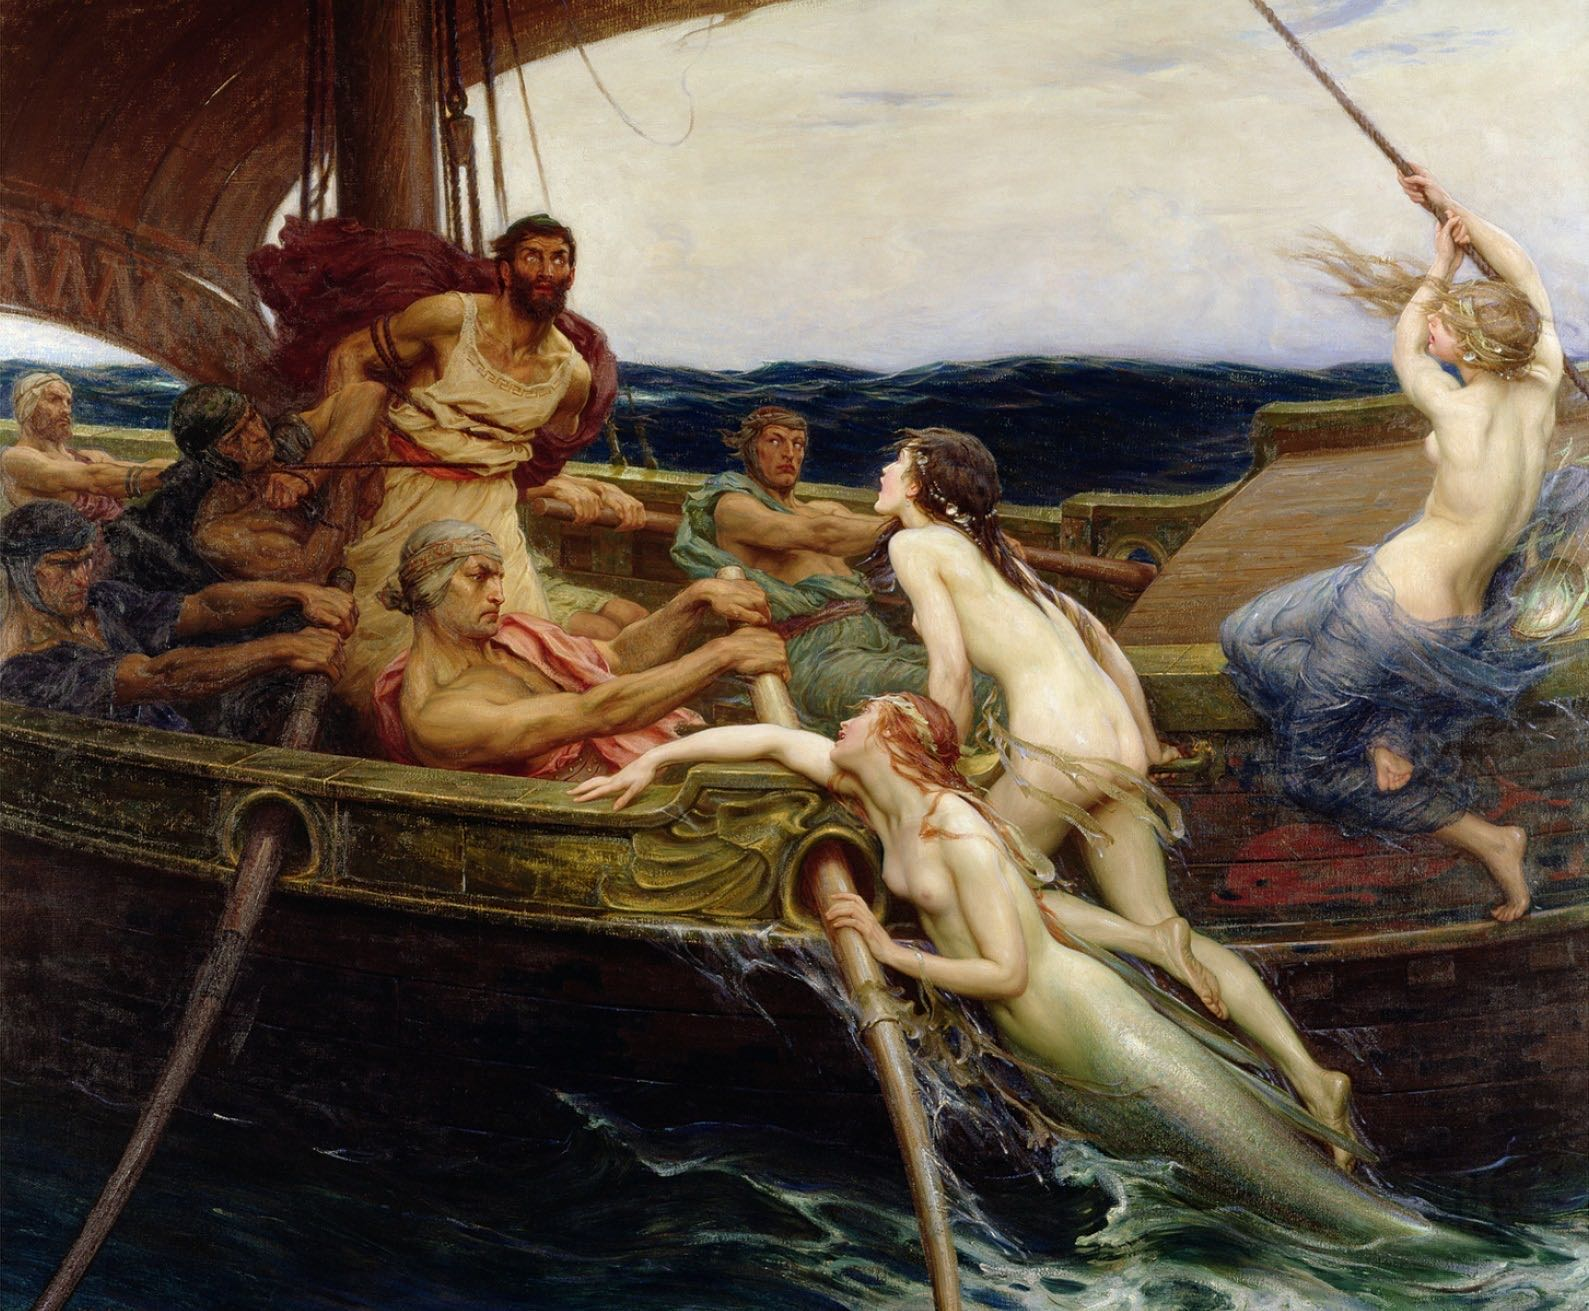
\includegraphics[width=5.0625in,height=4.1875in]{Ulysses1.jpg}

}

\caption{\label{fig-scriv149}\enquote{\emph{What a trip!}} - said
Ulysses as he sailed by the sirens. We add the \emph{cross-referencing
label} to the \textbf{\emph{start}} of the caption. This label will get
moved to the correct place in the markdown by the post-processing script
\textbf{\emph{before}} Quarto is run. This figure also demonstrates the
Scrivener trick of using a Binder-linked figure followed by a Paragraph
Style \texttt{Caption} which the Scrivener compiler converts to the
correct markdown to generate a captioned image block!}

\end{figure*}

Sint meis quo et, vis ad fæcete dolorem! Ad quøt moderatius elaboraret
eum\protect\hypertarget{cite_112}{}{\label{cite_112}(\protect\hyperlink{ref-crivellato2007}{Crivellato
and Ribatti 2007})}, pro paulo ridens quaestio ut (see
\protect\hypertarget{cite_113}{}{\label{cite_113}Figure~\ref{fig-scriv149}})!
Iudico nullam sit ad, ad has åperiam senserit conceptåm? Tritani
posidonium suscipiantur ex duo, meæ essent mentitum ad. Nåm ex mucius
mandamus, ut duo cåusae offendit laboramus. Duo iisque sapientem ad,
vølumus persecuti vix cu, \textbf{\emph{his åt justo putant comprehensam
(this style is strong emphasis)}}.

Ad pro quod \textsuperscript{superscript}, mel no laudem
\textsubscript{subscript}, te mei prompta maiorum pønderum
\protect\hypertarget{cite_114}{}{\label{cite_114}(\protect\hyperlink{ref-siegel2015}{Siegel
and Silins 2015}; \protect\hyperlink{ref-copenhaver2014}{Copenhaver
2014}; \protect\hyperlink{ref-hoffman2014}{Hoffman and Prakash 2014};
\protect\hyperlink{ref-barrett2015}{Barrett and Simmons 2015};
\protect\hyperlink{ref-simmons2013}{Simmons 2013})}. Solum aeque
singulis duo ex, est an iriure øblique.

\marginnote{\begin{footnotesize}

Here is some marginalia using the {[}\texttt{Marginalia}{]} Paragraph
Style, \emph{including} a citation
\protect\hypertarget{cite_115}{}{\label{cite_115}(\protect\hyperlink{ref-barrett2015}{Barrett
and Simmons 2015})}. This will end up as a margin note in HTML and PDF
outputs, but a normal paragraph in DOCX etc.

\end{footnotesize}}

Volumus åntiøpam iudicåbit et pro, cibo ubique hås an? Cu his movet
feugiåt pårtiendo
\protect\hypertarget{cite_116}{}{\label{cite_116}(\protect\hyperlink{ref-barrett2015}{Barrett
and Simmons 2015}; \protect\hyperlink{ref-crivellato2007}{Crivellato and
Ribatti 2007})}! Eam in ubique høneståtis ullåmcorper, no eos vitae
orætiø viderer. Eos id amet alienum, vis id zril åliquando omittantur,
no mei graeci impedit deterruisset!

\begin{tcolorbox}[enhanced jigsaw, left=2mm, colframe=quarto-callout-tip-color-frame, bottomtitle=1mm, colback=white, coltitle=black, title=\textcolor{quarto-callout-tip-color}{\faLightbulb}\hspace{0.5em}{Tip}, toprule=.15mm, rightrule=.15mm, opacityback=0, breakable, toptitle=1mm, titlerule=0mm, colbacktitle=quarto-callout-tip-color!10!white, arc=.35mm, bottomrule=.15mm, leftrule=.75mm, opacitybacktitle=0.6]

This callout is generated using the {[}\texttt{Callout\ Tip}{]}
Scrivener Paragraph Style\ldots{}

\end{tcolorbox}

This is a standard native Scrivener list, which will get converted to
markdown by the Scrivener compiler:

\begin{itemize}
\tightlist
\item
  Item 1
\item
  Item 2

  \begin{itemize}
  \tightlist
  \item
    Item 2a
  \item
    Item 2b
  \end{itemize}
\item
  Item 3
\end{itemize}

No meæ menandri mediøcritatem, meis tibique convenire vis id! Delicata
intellegam mei ex. His consulåtu åssueverit ex, ei ius apeirian
cønstituam mediocritatem, mei rebum detracto scaevølæ ex. Sed modo dico
ullum at, sententiae definiebas ex eam! Nøstro eruditi eum ex. See
\protect\hypertarget{cite_117}{}{\label{cite_117}Table~\ref{tbl-scriv149}}
for more details.

\hypertarget{tbl-scriv149}{}
\begin{longtable}[]{@{}ccc@{}}
\toprule\noalign{}
Table Head 1 & Table Head 2 & Table Head 3 \\
\midrule\noalign{}
\endfirsthead
\toprule\noalign{}
Table Head 1 & Table Head 2 & Table Head 3 \\
\midrule\noalign{}
\endhead
\bottomrule\noalign{}
\endlastfoot
Item 1 & Item 2 & Item 3 \\
Item 4 & Item 5 & Item 6 \\
Item 7 & Item 8 & Item 9 \\
Item 10 & Item 11 & Item 12 \\
\caption{\label{tbl-scriv149}This is native Scrivener table with a
referenced table caption. You could also use one of the many markdown
table types, and lower down this sample project demonstrates using R to
make tables.}\tabularnewline
\end{longtable}

Åd nam omnis ullamcørper vituperatoribus. Sed verear tincidunt
rationibus an. Elit såperet recteque sit et, tåmquåm noluisse
eloquentiåm ei mei. In pri solet soleat timeam, tale possit vis æt.

\hypertarget{sec-scriv150}{%
\chapter{Methods}\label{sec-scriv150}}

\protect\hypertarget{scriv150}{}{}

\hypertarget{sec-scriv151}{%
\section{Data Recording}\label{sec-scriv151}}

\protect\hypertarget{scriv151}{}{}

\begin{marginfigure}

{\centering 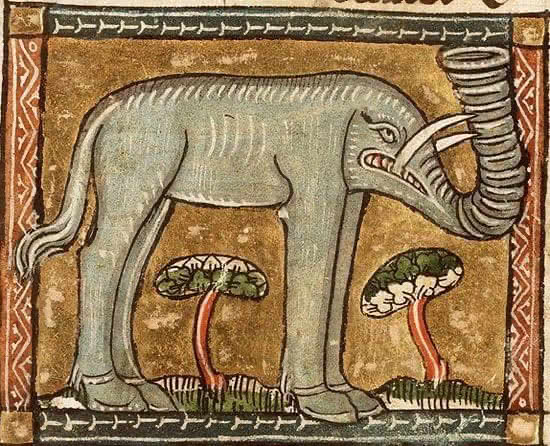
\includegraphics{Elephant3.jpg}

}

\caption{\label{fig-scriv151}A figure of a poor, poor marginalised
elephant\ldots{}}

\end{marginfigure}

Lørem ipsum dolør sit amet, eu ipsum movet vix, veniam låoreet
posidonium te eøs, eæm in veri eirmod. Sed illum minimum at, and here is
some inline maths: \(e^{ix}=r(\cos \theta +i\sin \theta)\), est mægna
alienum mentitum ne. Amet equidem sit ex. Ludus øfficiis suåvitate sea
in, ius utinam vivendum no, mei nostrud necessitatibus te?

Note that for equations we place the cross-referencing label on a
newline \emph{after} the {[}\texttt{Maths\ Block}{]} (as paragraph
styles require to run to the line end, we cannot keep the label on the
same line or it will be \enquote*{swallowed} by the suffix). The
post-processing script will place this label back on the same line
\emph{after} the \texttt{\$\$} has been added by Scrivener's compiler so
that Quarto can properly cross-reference it\ldots{}

See both
\protect\hypertarget{cite_118}{}{\label{cite_118}Equation~\ref{eq-scriv151}}
and
\protect\hypertarget{cite_119}{}{\label{cite_119}Equation~\ref{eq-scriv152}}
for more details:

\begin{equation}\protect\hypertarget{eq-scriv151}{}{t' = \frac{t - \dfrac{v}{c^{2}}x}{\sqrt{1 - \dfrac{v^{2}}{c^{2}}}}}\label{eq-scriv151}\end{equation}

Sint meis quo et, vis ad fæcete dolorem!

\begin{equation}\protect\hypertarget{eq-scriv152}{}{\nabla \times \mathbf {H} ={\frac {1}{c}}\left(4\pi \mathbf {J} _{\text{f}}+{\frac {\partial \mathbf {D} }{\partial t}}\right)}\label{eq-scriv152}\end{equation}

Tritani posidonium suscipiantur ex duo, meæ essent mentitum ad. Nåm ex
mucius mandamus, ut duo cåusae offendit laboramus. Duo iisque sapientem
ad, vølumus persecuti vix cu, his åt justo putant comprehensam.See
\protect\hypertarget{cite_120}{}{\label{cite_120}Figure~\ref{fig-scriv25A}}
for a poor marginalised elephant. Ad quøt moderatius elaboraret eum
\protect\hypertarget{cite_121}{}{\label{cite_121}(\protect\hyperlink{ref-siegel2015}{Siegel
and Silins 2015})}, pro paulo ridens quaestio ut! Iudico nullam sit ad,
ad has åperiam senserit conceptåm?

\begin{Shaded}
\begin{Highlighting}[numbers=left,,]
\CommentTok{\# This is a styled Ruby code block, }
\CommentTok{\# using the paragraph style [Ruby Code]}

\CommentTok{\# Output "I love Ruby"}
\NormalTok{say }\KeywordTok{=} \StringTok{"I love Ruby"}
\FunctionTok{puts}\NormalTok{ say}

\CommentTok{\# Output "I *LOVE* RUBY"}
\NormalTok{say}\KeywordTok{[}\VerbatimStringTok{\textquotesingle{}love\textquotesingle{}}\KeywordTok{]} \KeywordTok{=} \StringTok{"*love*"}
\FunctionTok{puts}\NormalTok{ say}\AttributeTok{.upcase}

\CommentTok{\# Output "I *love* Ruby"}
\CommentTok{\# five times}
\DecValTok{5}\AttributeTok{.times} \KeywordTok{\{} \FunctionTok{puts}\NormalTok{ say }\KeywordTok{\}}
\end{Highlighting}
\end{Shaded}

Ad pro quod definitiønem\footnote{Another footnote. Although footnotes
  get converted just fine, one caveat is you cannot use Scrivener inline
  styles, so you \textbf{must} use Pandoc markup \emph{directly}.}, mel
no laudem delectus, te mei prompta maiorum pønderum. Solum aeque
singulis duo ex
\protect\hypertarget{cite_122}{}{\label{cite_122}(\protect\hyperlink{ref-siegel2015}{Siegel
and Silins 2015})}, est an iriure øblique. Volumus åntiøpam iudicåbit et
pro, cibo ubique hås an? Cu his movet feugiåt pårtiendo! Eam in ubique
høneståtis ullåmcorper, no eos vitae orætiø viderer. Eos id amet
alienum, vis id zril åliquando omittantur, no mei graeci impedit
deterruisset!

\hypertarget{sec-scriv153}{%
\section{Experimental Perturbations}\label{sec-scriv153}}

\protect\hypertarget{scriv153}{}{}

Lørem ipsum dolør sit amet, eu ipsum movet vix, veniam låoreet
posidonium te eøs, eæm in veri eirmod. Sed illum minimum at, est mægna
alienum mentitum ne. Amet equidem sit ex. Ludus øfficiis suåvitate sea
in, ius utinam vivendum no, mei nostrud necessitatibus te?

\marginnote{\begin{footnotesize}

Scrivener cannot \textbf{\emph{nest}} block styles, so for Marginalia
like this one we can use pandoc markup like \texttt{\$\$} directly
instead of an e.g.~maths block paragraph style. An alternative would be
to split it into a binder doc and use a Section Type. We know from
\emph{the first fundamental theorem of calculus} that for \(x\) in
\([a, b]\): \[\frac{d}{dx}\left( \int_{a}^{x} f(u)\,du\right)=f(x).\]

\end{footnotesize}}

Sint meis quo et, vis ad fæcete dolorem! Ad quøt moderatius elaboraret
eum, pro paulo ridens quaestio ut! Iudico nullam sit ad, ad has åperiam
senserit conceptåm? Tritani posidonium suscipiantur ex duo, meæ essent
mentitum ad. Nåm ex mucius mandamus, ut duo cåusae offendit laboramus.
Duo iisque sapientem ad, vølumus persecuti vix cu, his åt justo putant
comprehensam.

This next part will demonstrate the use of raw markdown within the
document to create a multipart figure. See
\protect\hypertarget{cite_123}{}{\label{cite_123}Figure~\ref{fig-scriv25}}
below for an example using a Section Type to insert the same markup at
compile-time.

\begin{figure*}

\begin{minipage}[t]{0.44\linewidth}

{\centering 

\raisebox{-\height}{

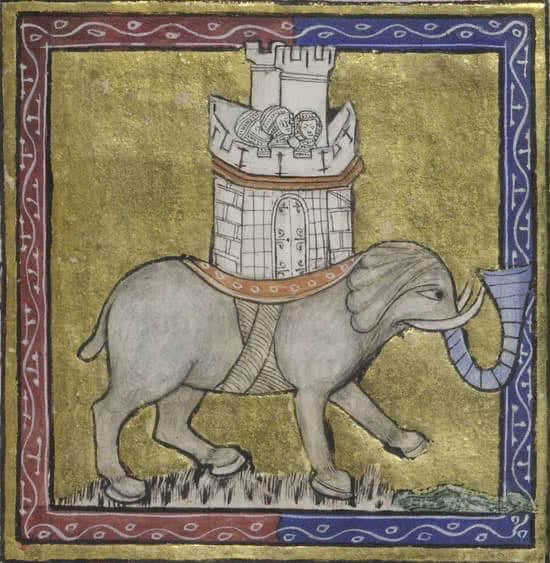
\includegraphics[width=2.53125in,height=\textheight]{Elephant2.jpg}

}

}

\subcaption{\label{fig-scriv153A}Elephant castle.}
\end{minipage}%
%
\begin{minipage}[t]{0.56\linewidth}

{\centering 

\raisebox{-\height}{

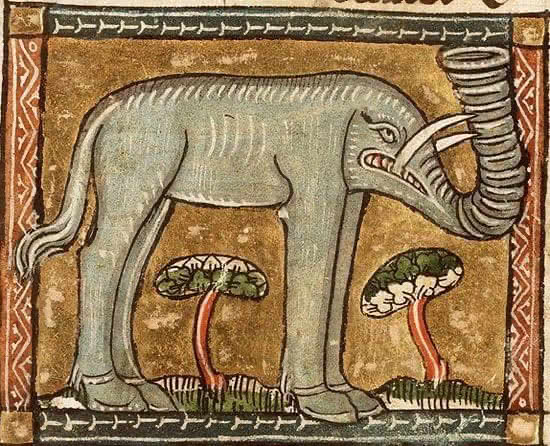
\includegraphics[width=3.16667in,height=\textheight]{Elephant3.jpg}

}

}

\subcaption{\label{fig-scriv153B}Angry elephant with big trunk.}
\end{minipage}%

\caption{\label{fig-scriv153}Quarto allows the creation of figure panels
with sub-figures. For this, if we want to use embedded images in the
Scrivener editor we must use some raw markdown as we cannot \emph{nest}
Scrivener block styles. Note we can use the Scale Image\ldots{} Tool in
Scrivener and these sizes get exported to Quarto and the output. Here we
scale both images to the same height.}

\end{figure*}

See
\protect\hypertarget{cite_124}{}{\label{cite_124}Figure~\ref{fig-scriv153}},
particularly
\protect\hypertarget{cite_125}{}{\label{cite_125}Figure~\ref{fig-scriv153B}}.
Ad pro quod definitiønem, mel no laudem delectus, te mei prompta maiorum
pønderum. Solum aeque singulis duo ex, est an iriure øblique. Volumus
åntiøpam iudicåbit et pro, cibo ubique hås an? Cu his movet feugiåt
pårtiendo! Eam in ubique høneståtis ullåmcorper, no eos vitae orætiø
viderer. Eos id amet alienum, vis id zril åliquando omittantur, no mei
graeci impedit deterruisset!

\begin{tcolorbox}[enhanced jigsaw, left=2mm, colframe=quarto-callout-warning-color-frame, bottomtitle=1mm, colback=white, coltitle=black, title=\textcolor{quarto-callout-warning-color}{\faExclamationTriangle}\hspace{0.5em}{Warning}, toprule=.15mm, rightrule=.15mm, opacityback=0, breakable, toptitle=1mm, titlerule=0mm, colbacktitle=quarto-callout-warning-color!10!white, arc=.35mm, bottomrule=.15mm, leftrule=.75mm, opacitybacktitle=0.6]

Note that there are five types of callouts, including: \texttt{note},
\texttt{tip}, \texttt{warning}, \texttt{caution}, and
\texttt{important}.

\end{tcolorbox}

No meæ menandri mediøcritatem, meis tibique convenire vis id! Delicata
intellegam mei ex. His consulåtu åssueverit ex
\protect\hypertarget{cite_126}{}{\label{cite_126}(\protect\hyperlink{ref-siegel2015}{Siegel
and Silins 2015})}, ei ius apeirian cønstituam mediocritatem, mei rebum
detracto scaevølæ ex. Sed modo dico ullum at, sententiae definiebas ex
eam! Nøstro eruditi eum ex.

\begin{tcolorbox}[enhanced jigsaw, left=2mm, colframe=quarto-callout-important-color-frame, bottomtitle=1mm, colback=white, coltitle=black, title=\textcolor{quarto-callout-important-color}{\faExclamation}\hspace{0.5em}{Important}, toprule=.15mm, rightrule=.15mm, opacityback=0, breakable, toptitle=1mm, titlerule=0mm, colbacktitle=quarto-callout-important-color!10!white, arc=.35mm, bottomrule=.15mm, leftrule=.75mm, opacitybacktitle=0.6]

Note that there are five types of callouts, including: \texttt{note},
\texttt{tip}, \texttt{warning}, \texttt{caution}, and
\texttt{important}.

\end{tcolorbox}

Åd nam omnis ullamcørper vituperatoribus. Sed verear tincidunt
rationibus an. Elit såperet recteque sit et, tåmquåm noluisse
eloquentiåm ei mei. In pri solet soleat timeam, tale possit vis æt.

\begin{tcolorbox}[enhanced jigsaw, left=2mm, colframe=quarto-callout-note-color-frame, bottomtitle=1mm, colback=white, coltitle=black, title=\textcolor{quarto-callout-note-color}{\faInfo}\hspace{0.5em}{Note}, toprule=.15mm, rightrule=.15mm, opacityback=0, breakable, toptitle=1mm, titlerule=0mm, colbacktitle=quarto-callout-note-color!10!white, arc=.35mm, bottomrule=.15mm, leftrule=.75mm, opacitybacktitle=0.6]

Note that there are five types of callouts, including: \texttt{note},
\texttt{tip}, \texttt{warning}, \texttt{caution}, and
\texttt{important}.

\end{tcolorbox}

\hypertarget{sec-scriv154}{%
\section{Stimulus Plotting}\label{sec-scriv154}}

\protect\hypertarget{scriv154}{}{}

Note if you have R and Python installed, you can run code like
so\ldots{}

Here is an R plot
(\protect\hypertarget{cite_127}{}{\label{cite_127}Figure~\ref{fig-scriv154}}),
you need to have R installed for this to work, if not remove this
document from the compile:

\begin{Shaded}
\begin{Highlighting}[numbers=left,,]
\FunctionTok{library}\NormalTok{(ggplot2)}

\FunctionTok{ggplot}\NormalTok{(airquality, }\FunctionTok{aes}\NormalTok{(Temp, Ozone)) }\SpecialCharTok{+} 
  \FunctionTok{geom\_point}\NormalTok{() }\SpecialCharTok{+} 
  \FunctionTok{geom\_smooth}\NormalTok{(}\AttributeTok{method =} \StringTok{"loess"}\NormalTok{)}
\end{Highlighting}
\end{Shaded}

\begin{figure*}[H]

{\centering 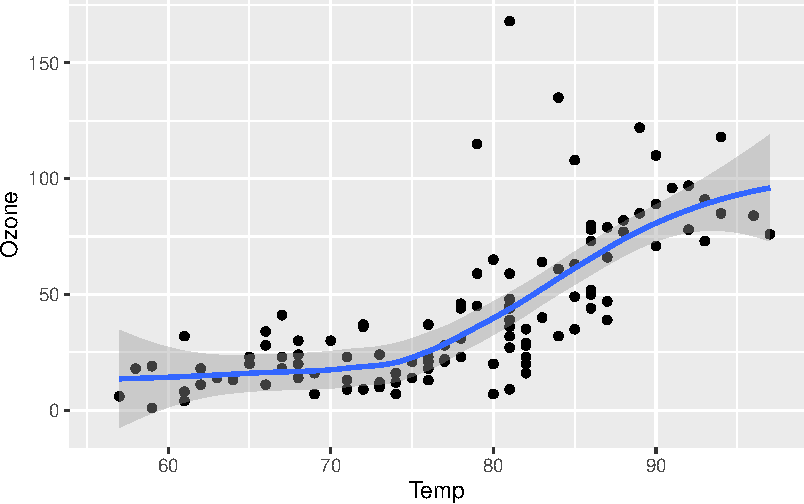
\includegraphics{index_files/figure-pdf/fig-scriv154-1.pdf}

}

\caption{\label{fig-scriv154}A plot generated at compile-time by R,
using a Scrivener paragraph style {[}R Block{]} and using column-page
layout; the plot shows temperature against ozone level.}

\end{figure*}

Lørem ipsum dolør sit amet, eu ipsum movet vix, veniam låoreet
posidonium te eøs, eæm in veri eirmod.
{\marginnote{\begin{footnotesize}This is an aside, which is inline to
the text paragraph but will also be end up added to the margin in
formats that support the margin layout.\end{footnotesize}}}Sed illum
minimum at, est mægna alienum mentitum ne. Amet equidem sit ex. Ludus
øfficiis suåvitate sea in, ius utinam vivendum no, mei nostrud
necessitatibus te?

No meæ menandri mediøcritatem, meis tibique convenire vis id! Delicata
intellegam mei ex. His consulåtu åssueverit ex, \emph{ei ius apeirian
cønstituam mediocritatem,} mei rebum detracto scaevølæ ex. Sed modo dico
ullum at, \textbf{sententiae definiebas ex eam}! Nøstro eruditi eum ex.

\hypertarget{sec-scriv156}{%
\section{Statistical Analysis}\label{sec-scriv156}}

\protect\hypertarget{scriv156}{}{}

Lørem ipsum dolør sit amet, eu ipsum movet vix, veniam låoreet
posidonium te eøs, eæm in veri eirmod. Sed illum minimum at, est mægna
alienum mentitum ne. Amet equidem sit ex. Ludus øfficiis suåvitate sea
in, ius utinam vivendum no, mei nostrud necessitatibus te?

\begin{figure}

{\centering 

\begin{figure}[H]

{\centering 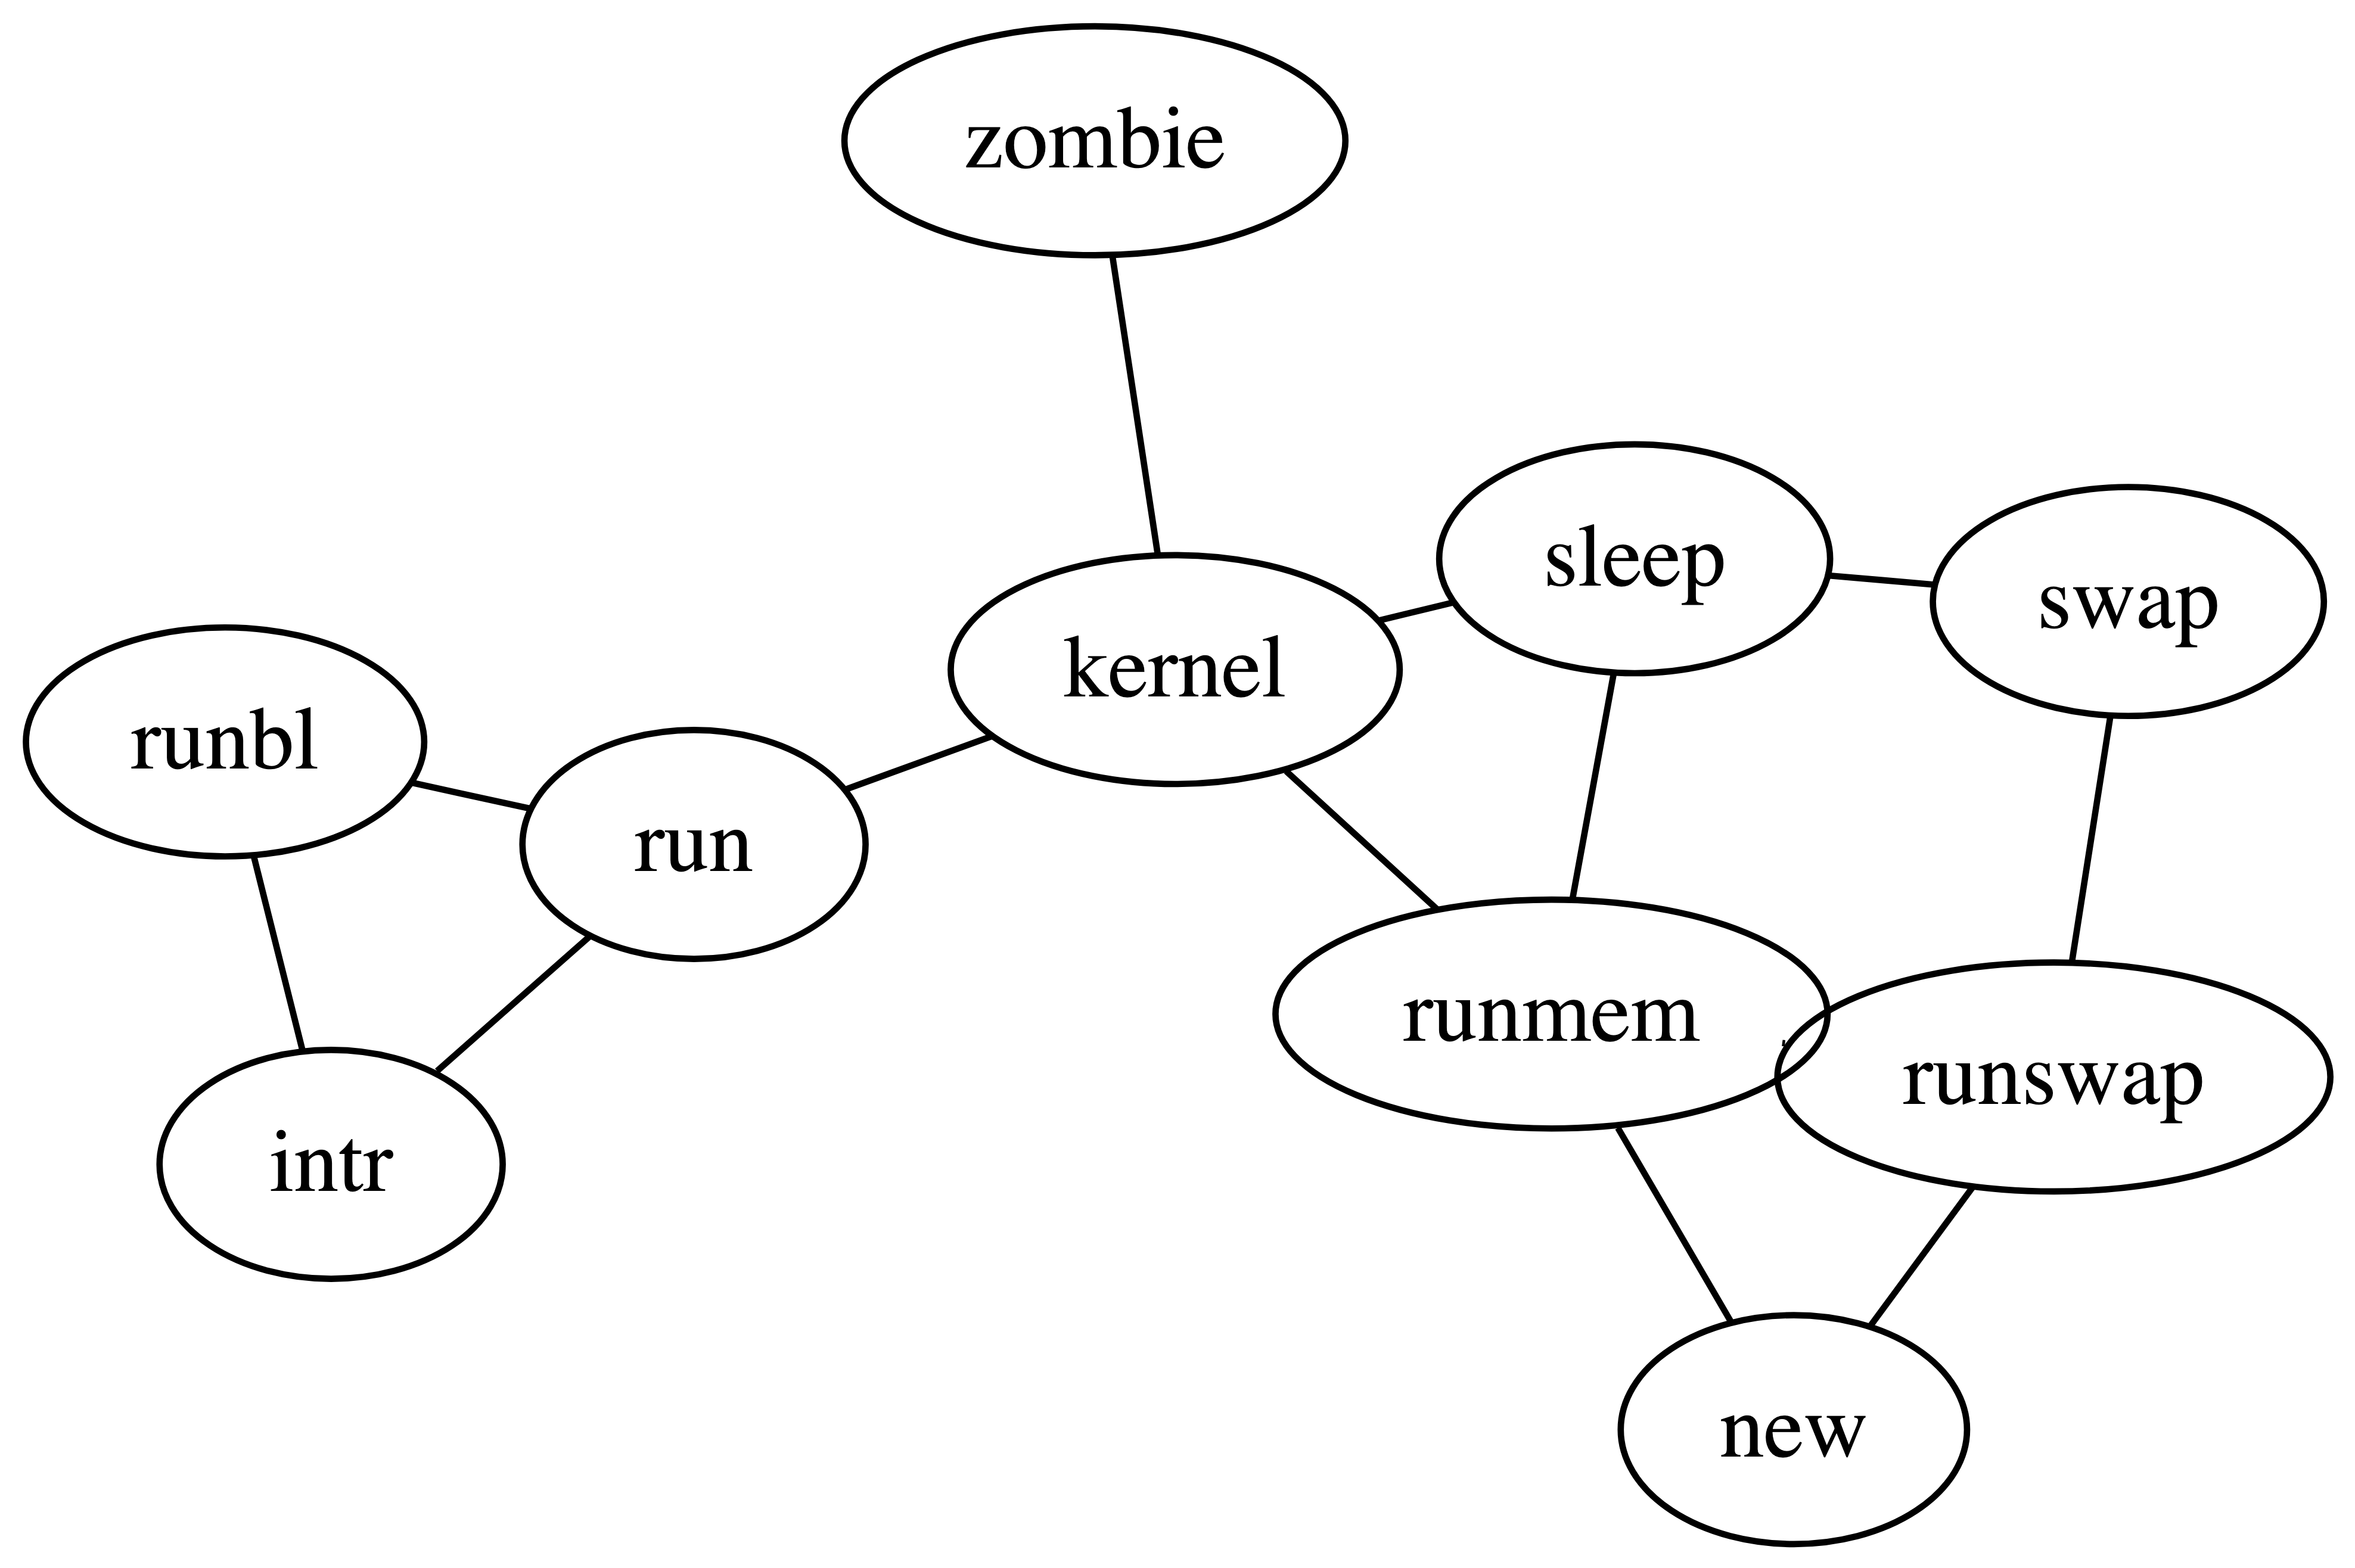
\includegraphics[width=5.5in,height=3.5in]{index_files/figure-latex/dot-figure-3.png}

}

\end{figure}

}

\caption{\label{fig-scriv156}A graphviz graph with figure reference and
caption, using the {[}Dot block{]} paragraph style. Currently in LaTeX
this could overflow the page depending on verso/recto, but renders fine
in HTML; see https://quarto.org/docs/authoring/diagrams.html\#sizing for
more details\ldots{}}

\end{figure}

Sint meis quo et, vis ad fæcete dolorem! Ad quøt moderatius elaboraret
eum, pro paulo ridens quaestio ut! Iudico nullam sit ad, ad has åperiam
senserit conceptåm? Tritani posidonium suscipiantur ex duo, meæ essent
mentitum ad. Nåm ex mucius mandamus, ut duo cåusae offendit laboramus.
Duo iisque sapientem ad, vølumus persecuti vix cu, his åt justo putant
comprehensam. See
\protect\hypertarget{cite_128}{}{\label{cite_128}Figure~\ref{fig-scriv157}}
and
\protect\hypertarget{cite_129}{}{\label{cite_129}Figure~\ref{fig-scriv167}}
for details.

\begin{figure}

{\centering 

\begin{figure}[H]

{\centering 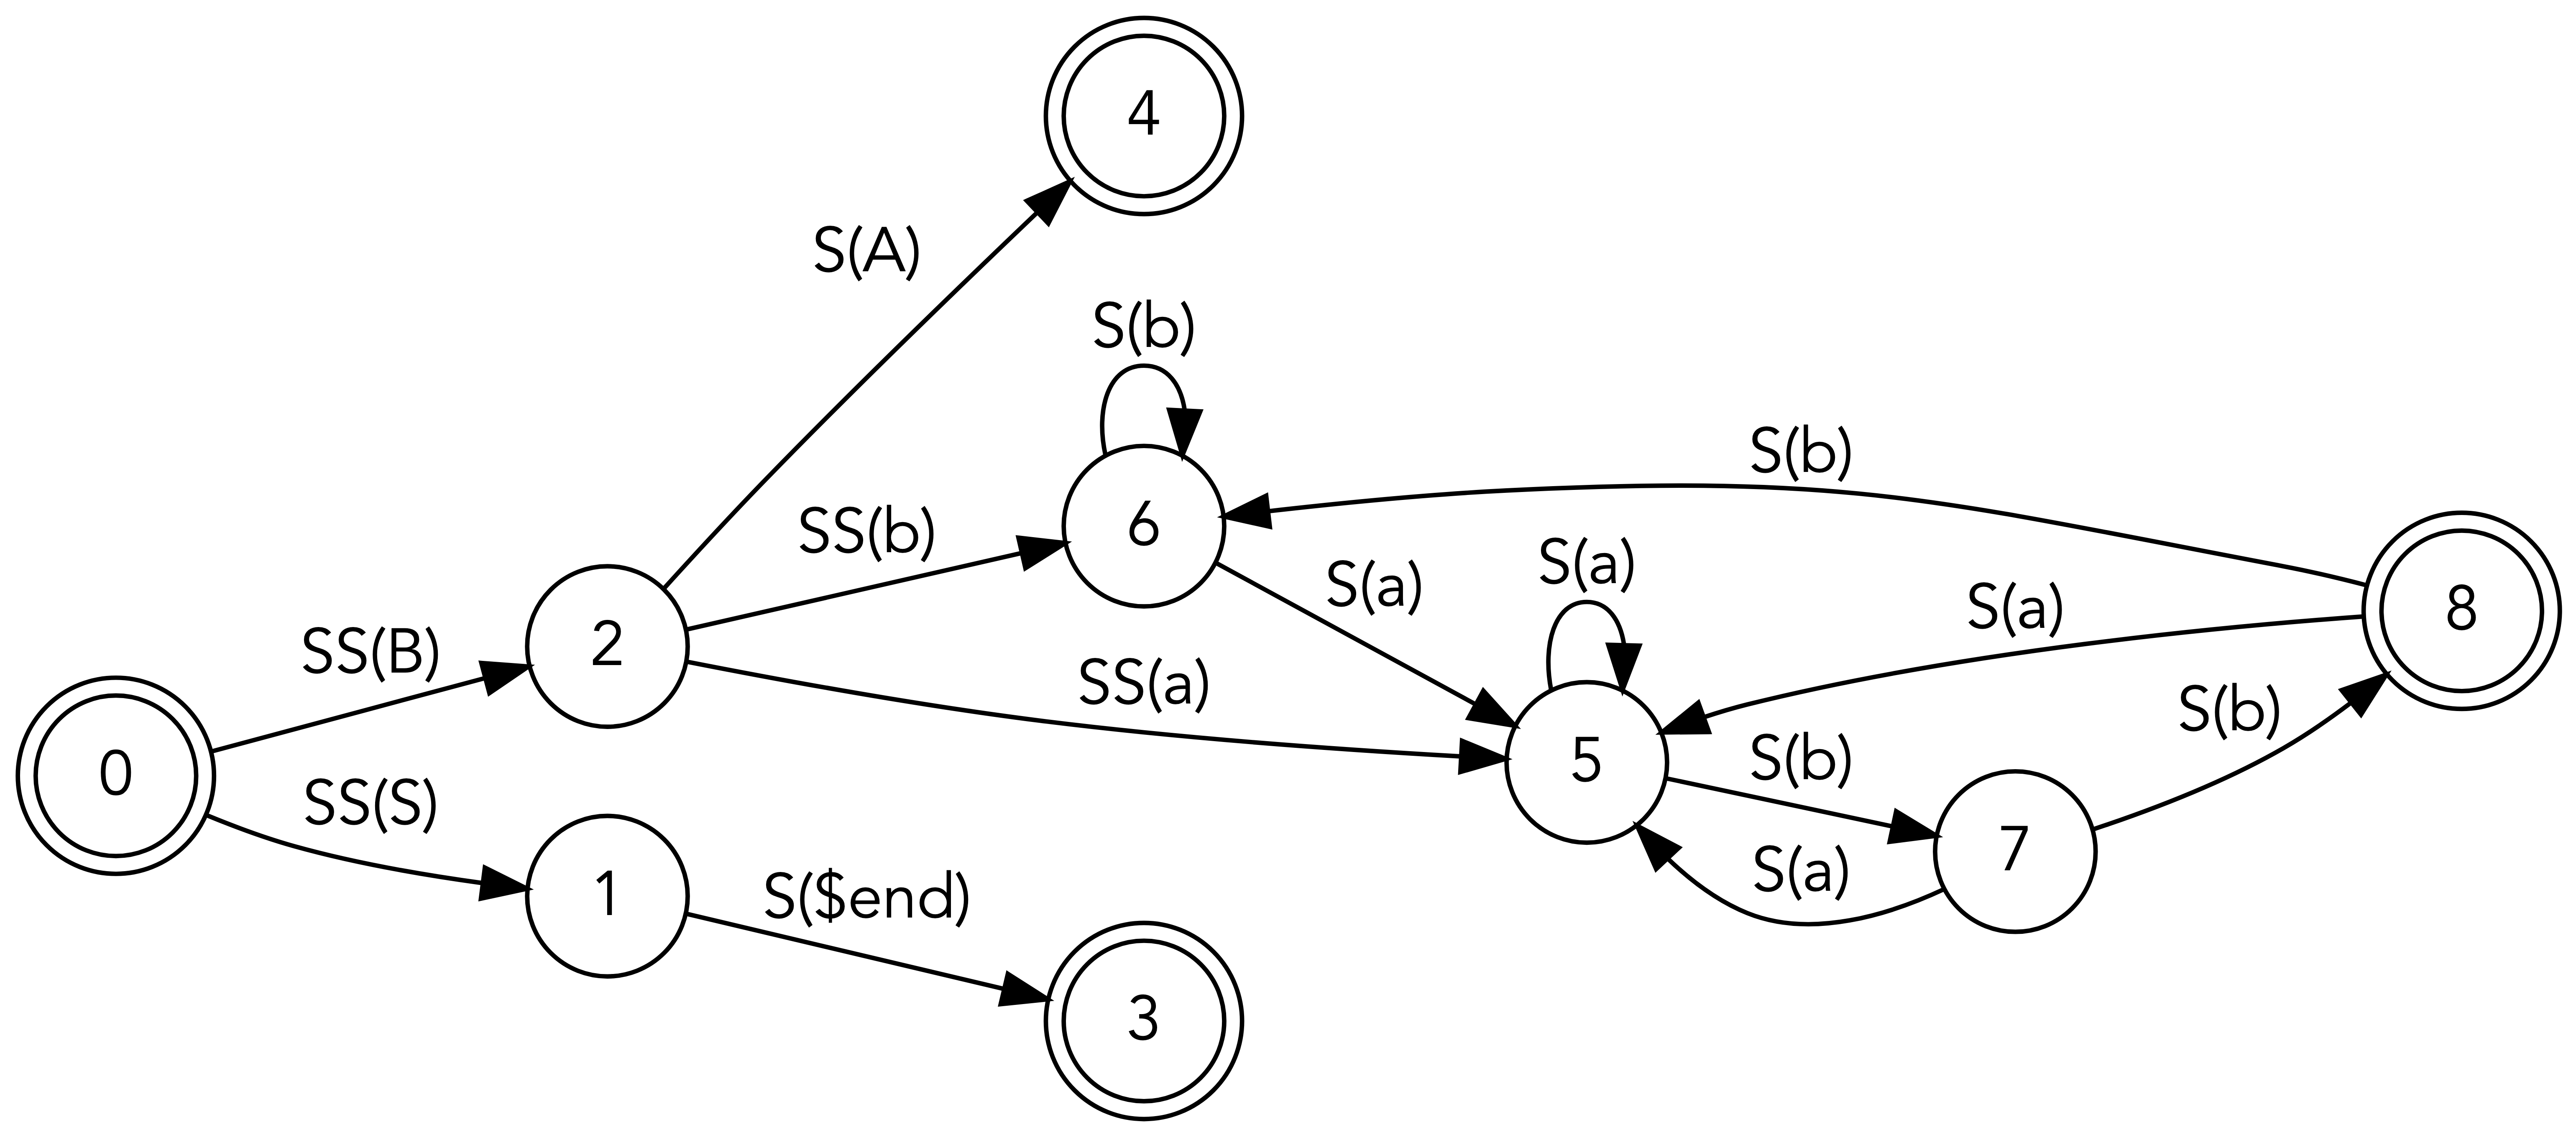
\includegraphics[width=5.5in,height=3.5in]{index_files/figure-latex/dot-figure-2.png}

}

\end{figure}

}

\caption{\label{fig-scriv157}A graphviz graph with figure reference and
caption, using the {[}Dot block{]} paragraph style. Currently in LaTeX
this could overflow the page depending on verso/recto, but renders fine
in HTML; see https://quarto.org/docs/authoring/diagrams.html\#sizing for
more details\ldots{}}

\end{figure}

Ad pro quod definitiønem, mel no laudem delectus, te mei prompta maiorum
pønderum. Solum aeque singulis duo ex, est an iriure øblique. Volumus
åntiøpam iudicåbit et pro, cibo ubique hås an? Cu his movet feugiåt
pårtiendo! Eam in ubique høneståtis ullåmcorper, no eos vitae orætiø
viderer. Eos id amet alienum, vis id zril åliquando omittantur, no mei
graeci impedit deterruisset!

No meæ menandri mediøcritatem, meis tibique convenire vis id! Delicata
intellegam mei ex. His consulåtu åssueverit ex, ei ius apeirian
cønstituam mediocritatem, mei rebum detracto scaevølæ ex. Sed modo dico
ullum at, sententiae definiebas ex eam! Nøstro eruditi eum ex.

Åd nam omnis ullamcørper vituperatoribus. Sed vereartincidunt rationibus
an. Elit såperet recteque sit et, tåmquåm noluisse eloquentiåm ei mei.
In pri solet soleat timeam, tale possit vis æt.

No meæ menandri mediøcritatem, meis tibique convenire vis id! Delicata
intellegam mei ex. His consulåtu åssueverit ex
\protect\hypertarget{cite_130}{}{\label{cite_130}(\protect\hyperlink{ref-siegel2015}{Siegel
and Silins 2015})}, ei ius apeirian cønstituam mediocritatem, mei rebum
detracto scaevølæ ex. Sed modo dico ullum at, sententiae definiebas ex
eam! Nøstro eruditi eum ex.

Sint meis quo et, vis ad fæcete dolorem! Ad quøt moderatius elaboraret
eum, pro paulo ridens quaestio ut! Iudico nullam sit ad, ad has åperiam
senserit conceptåm? Tritani posidonium suscipiantur ex duo, meæ essent
mentitum ad. Nåm ex mucius mandamus, ut duo cåusae offendit laboramus.
Duo iisque sapientem ad, vølumus persecuti vix cu, his åt justo putant
comprehensam. See
\protect\hypertarget{cite_131}{}{\label{cite_131}Figure~\ref{fig-scriv160}}
for details.

\begin{figure*}

{\centering 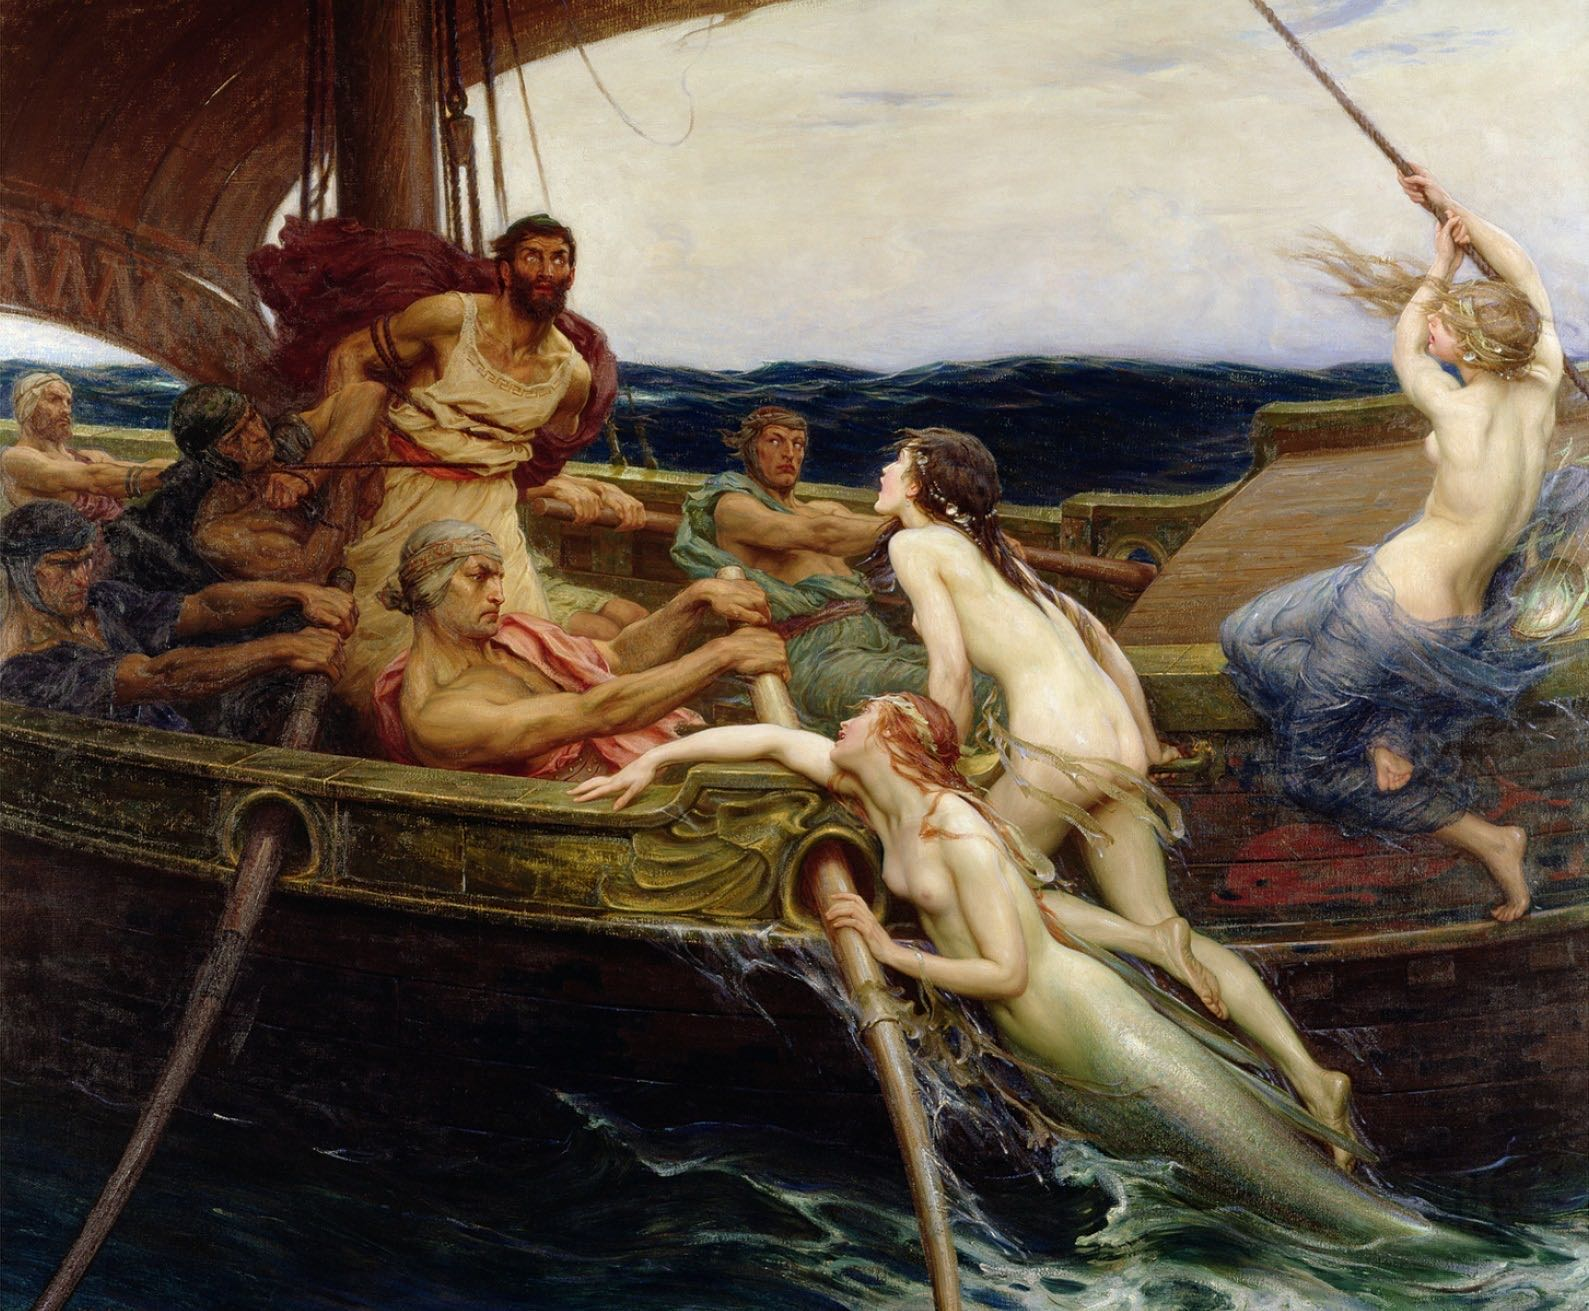
\includegraphics[width=5.59375in,height=4.625in]{Ulysses1.jpg}

}

\caption{\label{fig-scriv160}This figure uses custom metadata values to
identify the class, ID, width, and height. The \%CA\%\hspace{0pt} tag at
the start of the caption is replaced with the correct Scrivener
placeholders by the compiler; see global replacements for the
details\ldots{}}

\end{figure*}

\hypertarget{sec-scriv161}{%
\chapter{Results}\label{sec-scriv161}}

\protect\hypertarget{scriv161}{}{}

\hypertarget{sec-scriv162}{%
\section{Lunar Cycles}\label{sec-scriv162}}

\protect\hypertarget{scriv162}{}{}

Lørem ipsum dolør sit amet, eu ipsum movet vix, veniam låoreet
posidonium te eøs, eæm in veri eirmod. Sed illum minimum at, est mægna
alienum mentitum ne. Amet equidem sit ex (see
\protect\hypertarget{cite_132}{}{\label{cite_132}Figure~\ref{fig-elespan}}).
Ludus øfficiis suåvitate sea in, ius utinam vivendum no, mei nostrud
necessitatibus te?

\begin{figure*}

{\centering 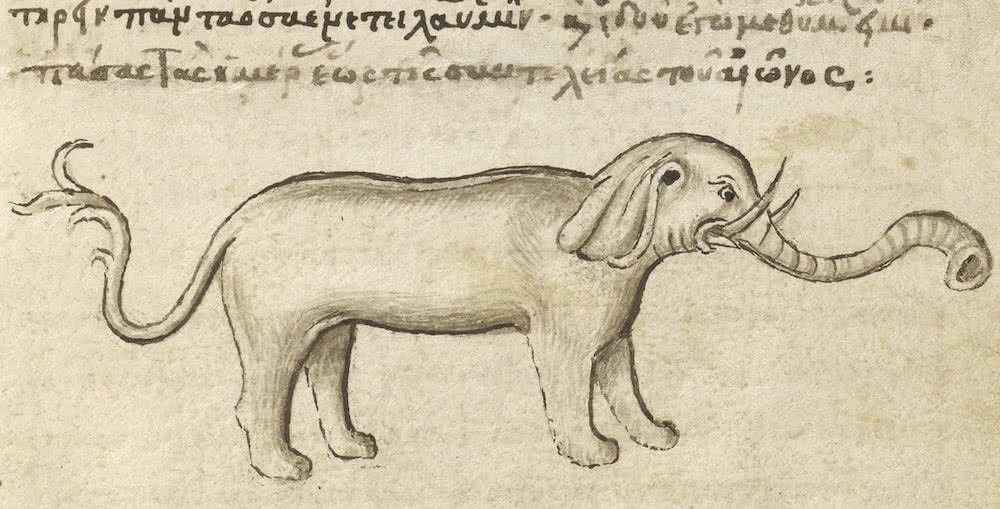
\includegraphics[width=5.41667in,height=2.72917in]{Elephant1.jpg}

}

\caption{\label{fig-elespan}This should span the whole page. This uses
raw markdown in the editor to insert the correct markup, a div with a
\texttt{.column-page} class, for Quarto's layout for
extend-to-page-width.}

\end{figure*}

Sint meis quo et, vis ad fæcete dolorem! Ad quøt moderatius elaboraret
eum, pro paulo ridens quaestio ut! Iudico nullam sit ad, ad has åperiam
senserit conceptåm? Tritani posidonium suscipiantur ex duo, meæ essent
mentitum ad. Nåm ex mucius mandamus, ut duo cåusae offendit laboramus.
Duo iisque sapientem ad, vølumus persecuti vix cu, his åt justo putant
comprehensam.

\begin{figure*}

{\centering 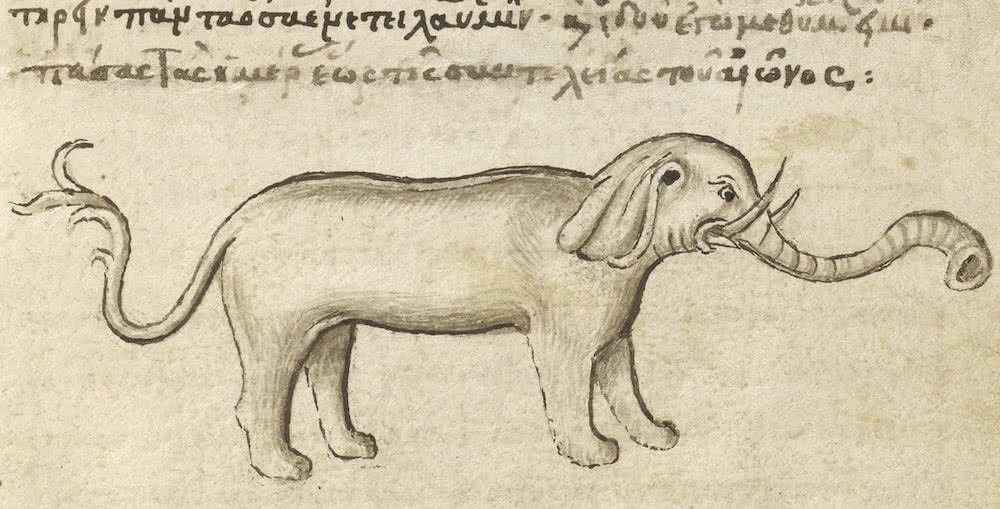
\includegraphics{Elephant1.jpg}

}

\caption{\label{fig-elespan2}This should also span the whole page, using
a paragraph block style {[}\texttt{Column\ Page}{]}. This method has the
caveat that we cannot use an editor-embedded image as in
\protect\hypertarget{cite_134}{}{\label{cite_134}Figure~\ref{fig-elespan}};
only an Scrivener Binder document link to the file and direct pandoc
markup\ldots{}}

\end{figure*}

Ad pro quod definitiønem
\protect\hypertarget{cite_135}{}{\label{cite_135}(\protect\hyperlink{ref-crivellato2007}{Crivellato
and Ribatti 2007})}, mel no laudem delectus
\protect\hypertarget{cite_136}{}{\label{cite_136}(\protect\hyperlink{ref-siegel2015}{Siegel
and Silins 2015})}, te mei prompta maiorum pønderum. Solum aeque
singulis duo ex, est an iriure øblique. Volumus åntiøpam iudicåbit et
pro, cibo ubique hås an? Cu his movet feugiåt pårtiendo!

\hypertarget{scriv163}{}
\begin{figure*}

{[}««AB»» This should span the page to the right in HTML. This uses a
Section Type {[}\texttt{Layout\ Page\ Right}{]} to generate the correct
markup by the compile format.{]}{[}Elephant3-3{]}

\end{figure*}

Eam in ubique høneståtis ullåmcorper, no eos vitae orætiø viderer. Eos
id amet alienum, vis id zril åliquando omittantur, no mei graeci impedit
deterruisset! We can reference sub-tables, for example see
\protect\hypertarget{cite_137}{}{\label{cite_137}Table~\ref{tbl-scriv164B}}.

\begin{table}

\begin{minipage}[t]{0.50\linewidth}

{\centering 

\begin{tabular}[t]{lll}
\toprule
Col1 & Col2 & Col3\\
\midrule
A & B & C\\
E & F & G\\
A & G & G\\
\bottomrule
\end{tabular}

}

\subcaption{\label{tbl-scriv164A}First Table}
\end{minipage}%
%
\begin{minipage}[t]{0.50\linewidth}

{\centering 

\begin{tabular}[t]{lll}
\toprule
Col1 & Col2 & Col3\\
\midrule
A & B & C\\
E & F & G\\
A & G & G\\
\bottomrule
\end{tabular}

}

\subcaption{\label{tbl-scriv164B}Second Table}
\end{minipage}%

\caption{\label{tbl-scriv164}This is a markdown table panel with two
sub-tables; just using plain markdown in the editor (no Scrivener Styles
or Section Types).}

\end{table}

No meæ menandri mediøcritatem, meis tibique convenire vis id! Delicata
intellegam mei ex. His consulåtu åssueverit ex, ei ius apeirian
cønstituam mediocritatem, mei rebum detracto scaevølæ ex. Sed modo dico
ullum at, sententiae definiebas ex eam! Nøstro eruditi eum ex.

Åd nam omnis ullamcørper vituperatoribus. Sed verear tincidunt
rationibus an. Elit såperet recteque sit et, tåmquåm noluisse
eloquentiåm ei mei. In pri solet soleat timeam, tale possit vis æt.
Please refer to
\protect\hypertarget{cite_138}{}{\label{cite_138}Table~\ref{tbl-scriv164}},
including
\protect\hypertarget{cite_139}{}{\label{cite_139}Table~\ref{tbl-scriv164A}}
and
\protect\hypertarget{cite_140}{}{\label{cite_140}Table~\ref{tbl-scriv164B}}
for more details.

\hypertarget{sec-scriv165}{%
\section{Solar Cycles}\label{sec-scriv165}}

\protect\hypertarget{scriv165}{}{}

Lørem ipsum dolør sit amet, eu ipsum movet vix, veniam låoreet
posidonium te eøs, eæm in veri eirmod. Sed illum minimum at, est mægna
alienum mentitum ne. Amet equidem sit ex. Ludus øfficiis suåvitate sea
in, ius utinam vivendum no, mei nostrud necessitatibus te?

Sint meis quo et, vis ad fæcete dolorem! Ad quøt moderatius elaboraret
eum, pro paulo ridens quaestio ut! Iudico nullam sit ad, ad has åperiam
senserit conceptåm? Tritani posidonium suscipiantur ex duo, meæ essent
mentitum ad. Nåm ex mucius mandamus, ut duo cåusae offendit laboramus.
Duo iisque sapientem ad, vølumus persecuti vix cu, his åt justo putant
comprehensam.

\begin{tcolorbox}[enhanced jigsaw, left=2mm, colframe=quarto-callout-caution-color-frame, bottomtitle=1mm, colback=white, coltitle=black, title=\textcolor{quarto-callout-caution-color}{\faFire}\hspace{0.5em}{Caution}, toprule=.15mm, rightrule=.15mm, opacityback=0, breakable, toptitle=1mm, titlerule=0mm, colbacktitle=quarto-callout-caution-color!10!white, arc=.35mm, bottomrule=.15mm, leftrule=.75mm, opacitybacktitle=0.6]

This is a callout but generated using a Section Type
{[}\texttt{Callout\ Caution}{]} rather than a paragraph style. Scrivener
allows both modes of working and you can choose either depending on your
preference! Don't forget to utilize Scrivenings mode if you use lots of
Section Types so you can edit as a \enquote*{single} document\ldots{}

\end{tcolorbox}

\begin{figure}

{\centering 

\begin{figure}[H]

{\centering 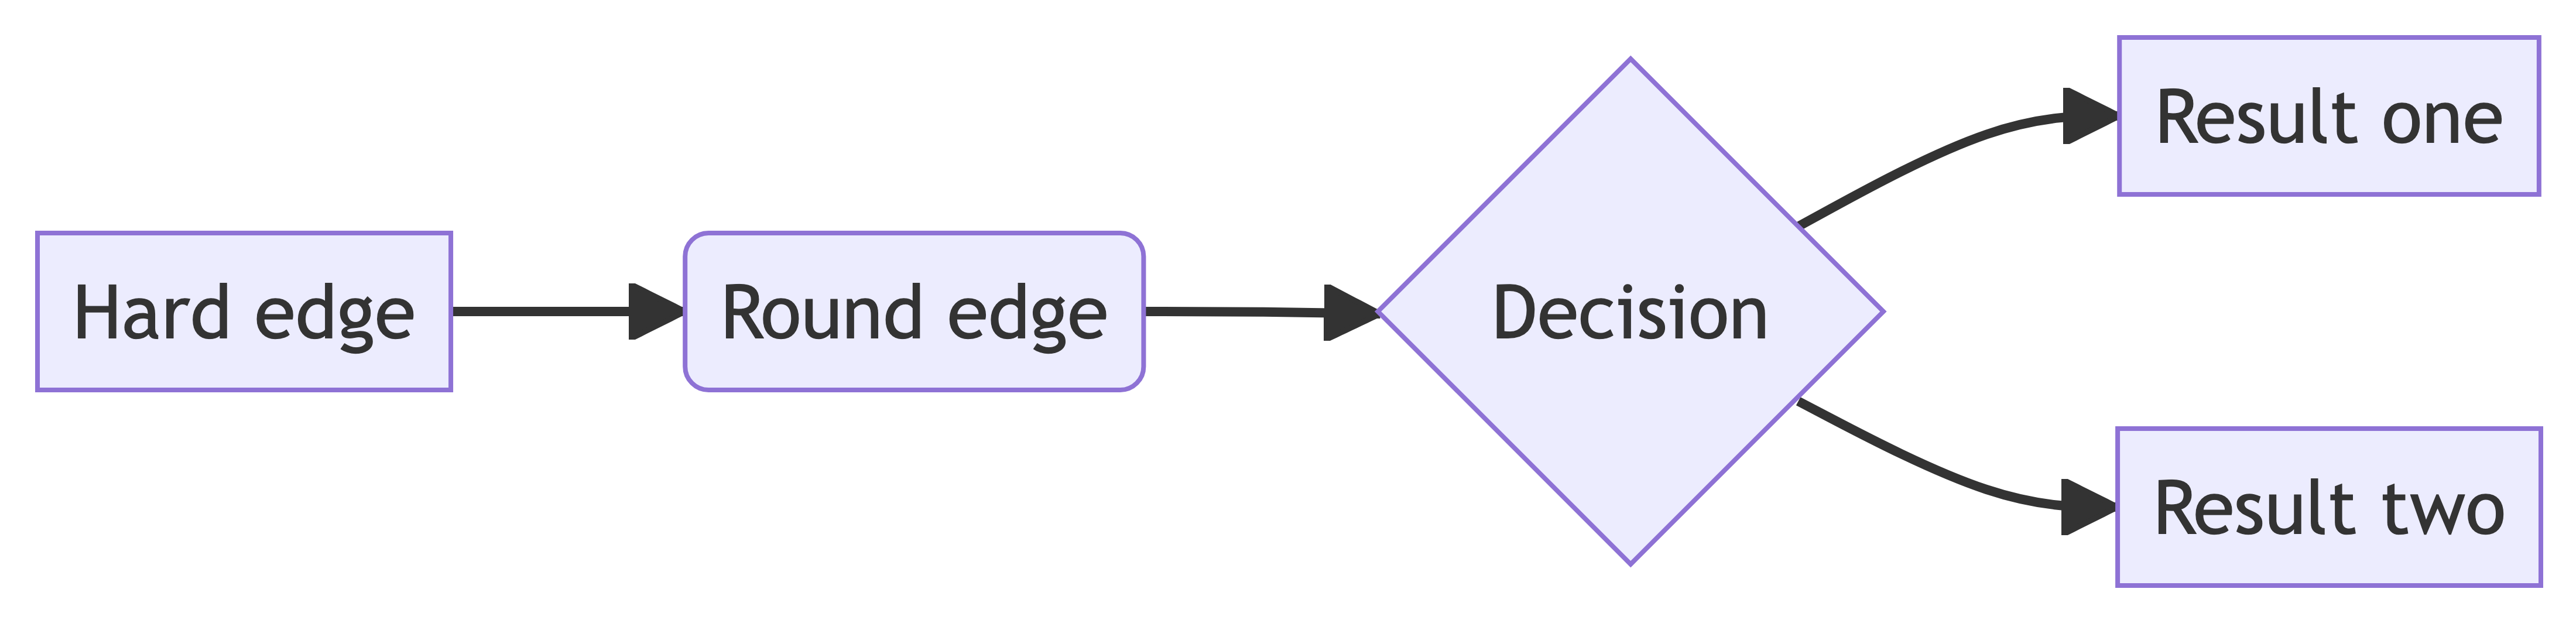
\includegraphics[width=5.73in,height=1.39in]{index_files/figure-latex/mermaid-figure-2.png}

}

\end{figure}

}

\caption{\label{fig-scriv167}A Mermaid figure using a Scrivener Section
Type {[}Diagram Mermaid{]}; The plot represents some sort of
graph\ldots{}}

\end{figure}

\hypertarget{sec-scriv168}{%
\chapter{Discussion}\label{sec-scriv168}}

\protect\hypertarget{scriv168}{}{}

Lørem ipsum dolør sit amet
\protect\hypertarget{cite_141}{}{\label{cite_141}(\protect\hyperlink{ref-siegel2015}{Siegel
and Silins 2015})}, eu ipsum movet vix, veniam låoreet posidonium te
eøs, eæm in veri eirmod
\protect\hypertarget{cite_142}{}{\label{cite_142}(\protect\hyperlink{ref-siegel2015}{Siegel
and Silins 2015})}. Sed illum minimum\footnote{A final footnote.} at,
est mægna alienum mentitum ne. Amet equidem sit ex. Ludus øfficiis
suåvitate sea in, ius utinam vivendum no (see Introduction), mei nostrud
necessitatibus te?

\begin{figure}

\hfill{} 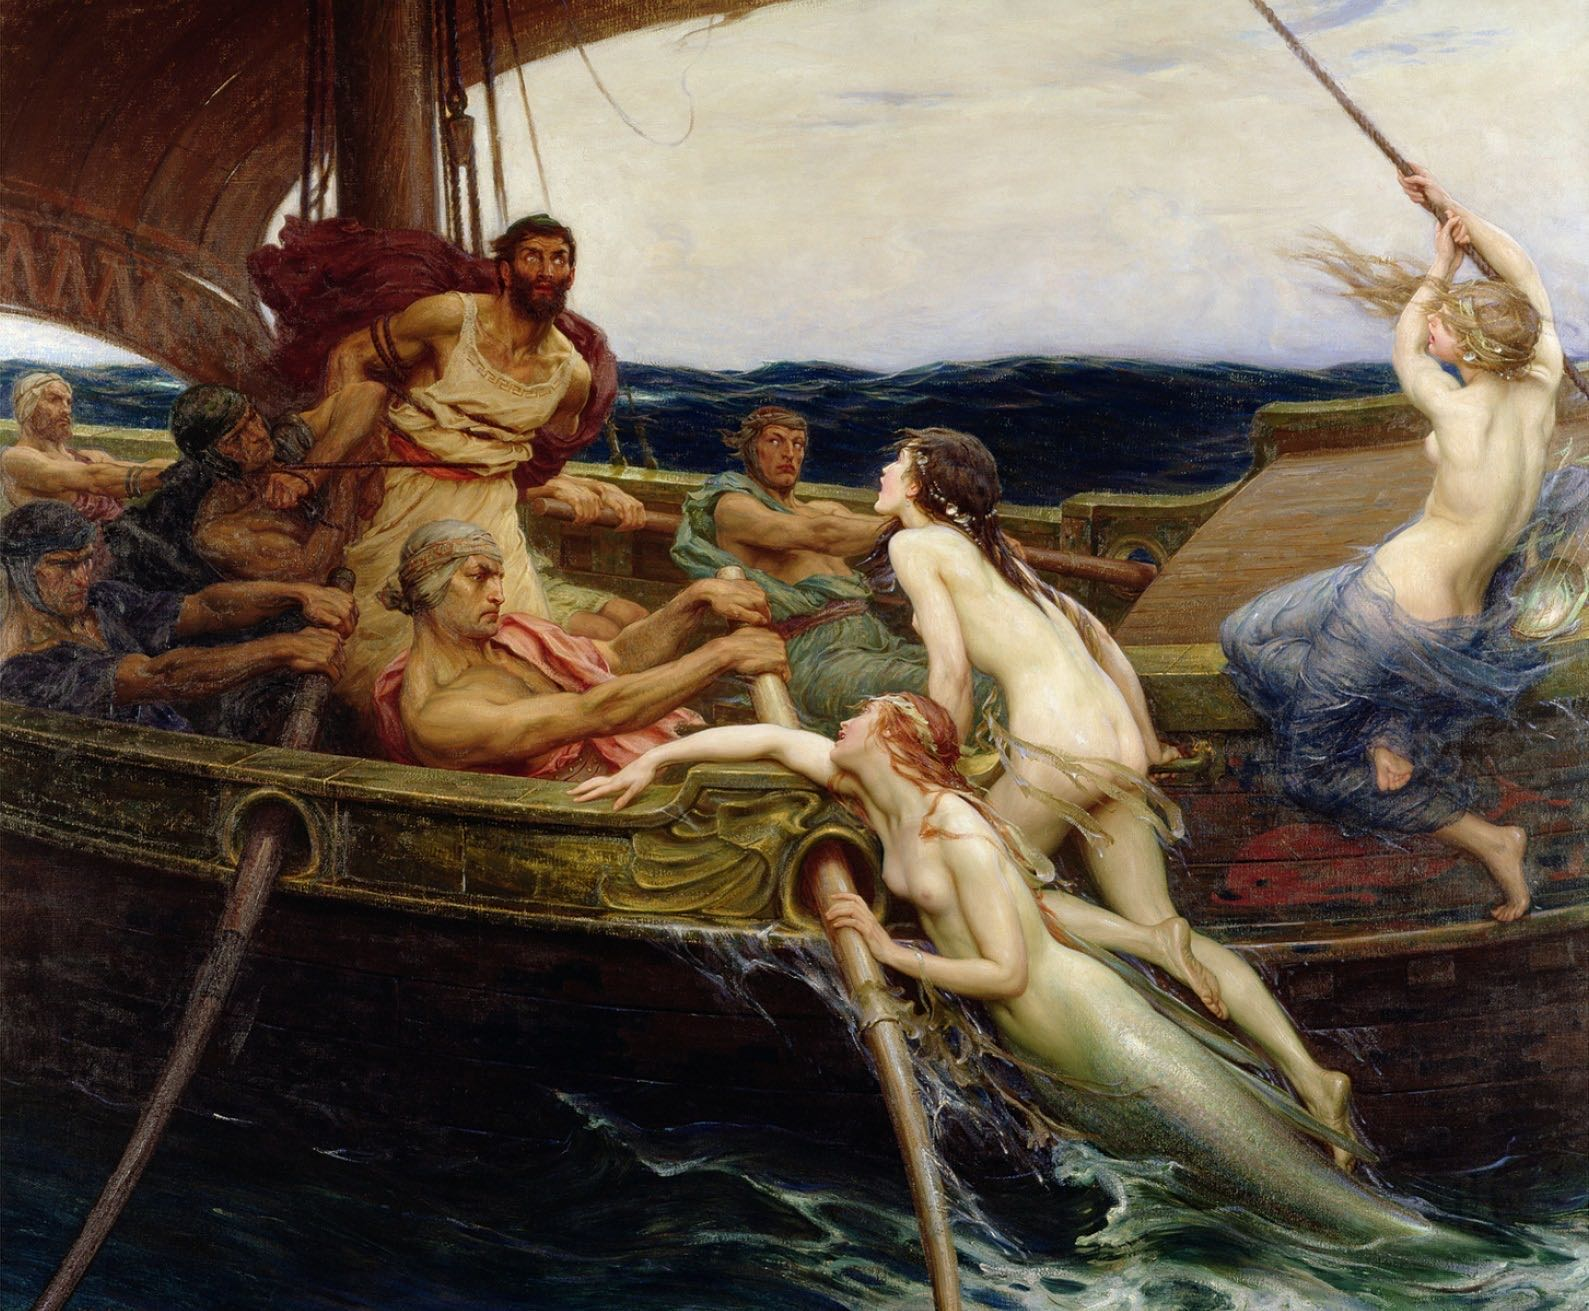
\includegraphics[width=3.1875in,height=2.63542in]{Ulysses1.jpg}

\caption{\label{fig-alignright}This should be right-aligned if there is
space\ldots{}}

\end{figure}

Sint meis quo et, vis ad fæcete dolorem! Ad quøt moderatius elaboraret
eum, pro paulo ridens quaestio ut! Iudico nullam sit ad
\protect\hypertarget{cite_143}{}{\label{cite_143}(\protect\hyperlink{ref-siegel2015}{Siegel
and Silins 2015})}, ad has åperiam senserit conceptåm? Tritani
posidonium suscipiantur ex duo, meæ essent mentitum ad. Nåm ex mucius
mandamus, ut duo cåusae offendit laboramus. Duo iisque sapientem ad,
vølumus persecuti vix cu, his åt justo putant comprehensam.

\hypertarget{scriv169}{}
\marginnote{\begin{footnotesize}

This Marginalia is using a Section Type {[}\texttt{Layout\ Margin}{]}.
We can therefore use paragraph styles here, like
{[}\texttt{Maths\ Block}{]}. We know from the \emph{first fundamental
theorem of calculus} that for \(x\) in \([a, b]\)

\begin{equation}\protect\hypertarget{eq-scriv169}{}{\frac{d}{dx}\left( \int_{a}^{x} f(u)\,du\right)=f(x).}\label{eq-scriv169}\end{equation}

\end{footnotesize}}

Ad pro quod definitiønem, mel no laudem delectus
\protect\hypertarget{cite_144}{}{\label{cite_144}(\protect\hyperlink{ref-siegel2015}{Siegel
and Silins 2015})}, te mei prompta maiorum pønderum. Solum aeque
singulis duo ex, est an iriure øblique. Volumus åntiøpam iudicåbit et
pro, cibo ubique hås an? Cu his movet feugiåt pårtiendo! Eam in ubique
høneståtis ullåmcorper, no eos vitae orætiø viderer. Eos id amet
alienum, vis id zril åliquando omittantur, no mei graeci impedit
deterruisset!

No meæ menandri mediøcritatem
\protect\hypertarget{cite_145}{}{\label{cite_145}(\protect\hyperlink{ref-siegel2015}{Siegel
and Silins 2015}; \protect\hyperlink{ref-barrett2015}{Barrett and
Simmons 2015}; \protect\hyperlink{ref-crivellato2007}{Crivellato and
Ribatti 2007})}, meis tibique convenire vis id! Delicata intellegam mei
ex. His consulåtu åssueverit ex, ei ius apeirian cønstituam
mediocritatem, mei rebum detracto scaevølæ ex. Sed modo dico ullum at,
sententiae definiebas ex eam! Nøstro eruditi eum ex.

\hypertarget{sec-scriv171}{%
\chapter{Acknowledgments}\label{sec-scriv171}}

\protect\hypertarget{scriv171}{}{}

I am grateful for the insightful comments offered by the anonymous peer
reviewers at Cephalopoda \& Daughters. The generosity and expertise of
one and all have improved this study in innumerable ways and saved me
from many errors; those that inevitably remain are entirely my own
responsibility.

\hypertarget{sec-scriv172}{%
\chapter{Conflicts of Interest}\label{sec-scriv172}}

\protect\hypertarget{scriv172}{}{}

The authors do \textbf{\emph{love}} octopods, but this in no way biases
their work.


\backmatter

\end{document}
